\documentclass[english]{book}
\usepackage[T1]{fontenc}
\usepackage[latin9]{inputenc}
\usepackage{geometry}
\geometry{verbose,tmargin=1in,bmargin=1in,lmargin=1in,rmargin=1in}
\pagestyle{headings}
\setcounter{secnumdepth}{3}
\setcounter{tocdepth}{5}
\usepackage{color}
\usepackage{babel}
\usepackage{array}
\usepackage{longtable}
\usepackage{varioref}
\usepackage{float}
\usepackage{textcomp}
\usepackage{url}
\usepackage{graphicx}
\usepackage{times}
\usepackage{textpos}
\usepackage[unicode=true]{hyperref}


\makeatletter

%%%%%%%%%%%%%%%%%%%%%%%%%%%%%% Textclass specific LaTeX commands.
\newenvironment{lyxcode}
{\par\begin{list}{}{
\setlength{\rightmargin}{\leftmargin}
\setlength{\listparindent}{0pt}% needed for AMS classes
\raggedright
\setlength{\itemsep}{0pt}
\setlength{\parsep}{0pt}
\normalfont\ttfamily}%
 \item[]}
{\end{list}}

%%%%%%%%%%%%%%%%%%%%%%%%%%%%%% User specified LaTeX commands.
\usepackage{hyperref}

\let\myUrl\url
\renewcommand{\url}[1]{(\myUrl{#1})}

\raggedbottom

\makeatother

\begin{document}

\definecolor{dark_grey}{gray}{0.3}
\definecolor{orange}{RGB}{255,177,20}

%LINE 1%
{
\renewcommand{\familydefault}{\sfdefault}

\pagenumbering{gobble}
\begin{center}
\resizebox{\textwidth}{!}{\textcolor{dark_grey}{\fontfamily{\sfdefault}\selectfont
COMPUTATIONAL INFRASTRUCTURE FOR GEODYNAMICS (CIG)
}}

%\hrule

\color{dark_grey}
\rule{\textwidth}{2pt}

\color{dark_grey}
{\Large }
\end{center}

\begin{center}
\resizebox{\textwidth}{!}{\colorbox
{orange}{\fontfamily{\rmdefault}\selectfont \textcolor{white} {
\hspace{0.05in}CitcomS\hspace{0.05in}
}}}
\end{center}

\begin{textblock*}{0in}(0in,-0.3in)
\begin{center}
\vspace{.2in}
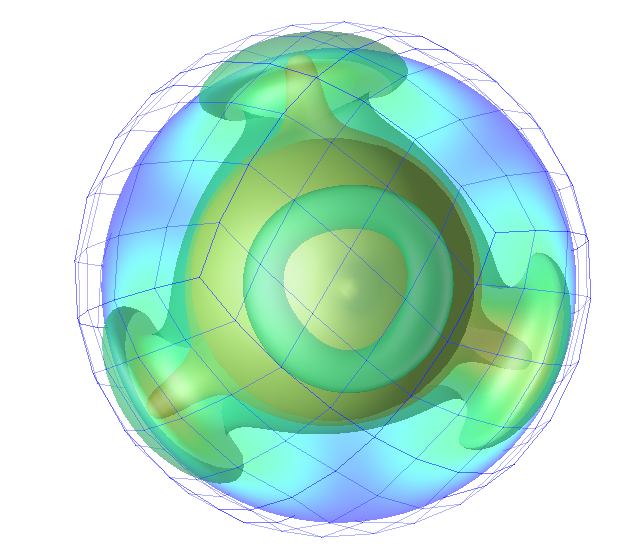
\includegraphics[height=5.5in]
{graphics/cookbook8.png}
\end{center}
\end{textblock*}

\color{dark_grey}
\hfill{\Huge \fontfamily{\sfdefault}\selectfont User Manual \\
\raggedleft \huge \fontfamily{\sfdefault}\selectfont Version {3.2.0}\\}

\null
\vfill
\color{dark_grey}
\Large \hfill {\raggedleft \fontfamily{\sfdefault}\selectfont
Eh Tan\\Michael Gurnis\\Luis Armendariz\\Leif Strand\\Susan Kientz\\
}
{\raggedright\fontfamily{\sfdefault}\selectfont www.geodynamics.org}

%\hrule
\vspace*{-0.275in}
%LINE%
\begin{center}
\color{dark_grey}
\rule{\textwidth}{2pt}
\end{center}
}

\pagebreak
\pagenumbering{arabic}

%\noindent \begin{center}
%\begin{figure}[H]
%\noindent \centering{}\includegraphics[width=0.75\paperwidth]{graphics/citcoms_cover.pdf}
%\end{figure}
%\par\end{center}
%\noindent \begin{center}
%\thispagestyle{empty}
%\par\end{center}
%\title{CitcomS User Manual}
%\author{� California Institute of Technology\\Version 3.2.0}

\title{CitcomS User Manual}
\date{\noindent \today}

\maketitle
\tableofcontents{}

\listoffigures



\part{Preface}


\chapter*{Preface}


\section*{About This Document}

This document is organized into three parts. Part I consists of traditional
book front matter, including this preface. Part II begins with an
introduction to Pyre and the Pyre-compatible version of CitcomS and
their capabilities and proceeds to the details of implementation,
including several ``cookbooks'' of short tutorials. Part III provides
appendices and references.

The style of this publication is based on the Apple Publications Style
Guide \url{developer.apple.com/documentation/UserExperience/Conceptual/APStyleGuide/AppleStyleGuide2003.pdf},
as recommended by Python.org \url{www.python.org}. The documentation
was produced using \LaTeX{}, specifically the \texttt{pdflatex} tool from the
TeXLive distribution \url{www.tug.org/texlive}.

Errors and bug fixes in this manual should be directed to the CIG
Mantle Convection Mailing List \url{cig-mc@geodynamics.org}.


\section*{Who Will Use This Document}

This documentation is aimed at two categories of users: scientists
who prefer to use prepackaged and specialized analysis tools, and
experienced computational Earth scientists. Of the latter, there are
likely to be two classes of users: those who just run models, and
those who modify the source code. Users who modify the source are
likely to have familiarity with scripting, software installation,
and programming, but are not necessarily professional programmers.

The manual was written for the usage of CitcomS on a variety of different
platforms. CitcomS has run on shared memory computers (Sun, Hewlett-Packard,
SGI, and IBM), commercial distributed memory machines (Intel and Cray/SGI),
clusters (including machines on the NSF TeraGrid), Linux PCs and Mac
OS X desktops. 


\section*{Citation}

Computational Infrastructure for Geodynamics (CIG) is making this
source code available to you in the hope that the software will enhance
your research in geophysics. The underlying C code for the finite
element package and the Python bindings for the framework were donated
to CIG in July of 2005. A number of individuals have contributed a
significant portion of their careers toward the development of CitcomS
and Pyre. It is essential that you recognize these individuals in
the normal scientific practice by citing the appropriate peer reviewed
papers and making appropriate acknowledgements. 

The CitcomS development team asks that you cite both of the following:
\begin{itemize}
\item Zhong, S., M.T. Zuber, L.N. Moresi, and M. Gurnis (2000), The role
of temperature-dependent viscosity and surface plates in spherical
shell models of mantle convection. \emph{J. Geophys. Res.,} \emph{105,}
11,063-11,082 
\item Tan, E., E. Choi, P. Thoutireddy, M. Gurnis, and M. Aivazis (2006),
GeoFramework: Coupling multiple models of mantle convection within
a computational framework,  \emph{Geochem., Geophys., Geosyst. 7,}
Q06001, doi:10.1029/2005GC001155. 
\end{itemize}
Additionally, if you are using tracers in CitcomS, please cite the
following:
\begin{itemize}
\item McNamara, A.K., and S. Zhong (2004), Thermochemical structures within
a spherical mantle: Superplumes or Piles?, \emph{J. Geophys. Res.},
109, B07402, doi:10.1029/2003JB002847.
\end{itemize}
The developers also request that in your oral presentations and in
your paper acknowledgements that you indicate your use of this code,
the authors of the code, and CIG \url{geodynamics.org}.


\section*{Support}

Pyre development is funded by the U.S. Dept. of Energy's Advanced
Simulation and Computing program \url{www.sandia.gov/NNSA/ASC} and
the National Science Foundation's \url{www.nsf.gov} Information Technology
Research (ITR) program (grant \#0205653). Continued support of CitcomS
is based upon work supported by the National Science Foundation under
Grant No. EAR-0406751. Any opinions, findings, and conclusions or
recommendations expressed in this material are those of the authors
and do not necessarily reflect the views of the National Science Foundation.


\section*{Conventions}

Throughout this documentation, any mention of ``username'' is meant
to indicate the user, meaning you should substitute your account name
in its place.


\part{Chapters}


\chapter{Introduction}

CitcomS is a finite element code designed to solve thermal convection
problems relevant to earth's mantle released under the GNU General
Public License (see Appendix \vref{cha:License}). Written in C, the
code runs on a variety of parallel processing computers, including
shared and distributed memory platforms. In an effort to increase
the functionality of CitcomS to include greater control during simulations
on large parallel systems, the software has been reengineered from
previous versions of CitcomS to work with a Python-based modeling
framework called Pyre. With Pyre, CitcomS can be dynamically coupled
with other CitcomS simulations or with other codes such as SNAC, which
solves crustal and lithospheric problems. 


\section{About CitcomS}

CitcomS is a finite element code written in C that solves for thermo-chemical
convection within a spherical shell. It can solve for problems within
either a full or a restricted spherical domain. Although the code
is capable of solving many different kinds of convection problems
using the flexibility of finite elements, there are aspects of CitcomS
which make it well-suited for solving problems in which the plate
tectonic history is incorporated. Variable viscosity, including temperature-,
pressure-, position-, composition-, and stress-dependent viscosity
are all possible. 

The fundamental basis for the numerical solution of any time-dependent
convection problem is the sequential solution of an equation of motion
and an energy equation. Convection problems are initially valued with
boundary conditions, including all of the problems which are solved
with CitcomS. The normal sequence of steps for the solution of convection
problems starts with an initial temperature field. First, the momentum
equation is solved. The solution of this equation gives us the velocity
from which we then solve the advection-diffusion equation, giving
us a new temperature. CitcomS uses this interleaved strategy. It is
possible to run convection backward in time so as to guess an initial
condition for a normal forward running initial and boundary value
problem. However, users should be aware that even specialists in mantle
convection modeling are just now starting to explore methods in this
area and, as such, this is an emerging area of research. 

This code uses an iterative solution scheme to solve for the velocity
and pressure and, as such, a converged solution cannot be guaranteed.
Nested inside the iterative scheme, the code uses either a conjugate
gradient solver or a full multi-grid solver to solve the discretized
matrix equations. 


\section{History}

Citcom (for \textbf{C}alifornia \textbf{I}nstitute of \textbf{T}echnology
\textbf{Co}nvection in the \textbf{M}antle) was originally written
in the early 1990s by Louis Moresi. Although the code for three-dimensional
problems was incorporated from its inception, early versions of the
software only solved for time-dependent convection problems within
two-dimensional Cartesian domains. Moresi's original code turned out
to be incredibly modular and easily extensible. Consequently, the
fundamental finite element infrastructure which Louis wrote is still
in place and forms the basis for much of the code contained in the
present release. 

In the mid-1990s Moresi wrote versions of the code that solved the
equations within three-dimensional Cartesian domains. Then Shijie
Zhong successfully parallelized Citcom using message passing routines
on a limited release Intel supercomputer. Zhong then created a spherical
version of the code which he named CitcomS. Lijie Han then created
a regional version of CitcomS as well as an alternate version of message
passing for an arbitrarily large number of processors. Clint Conrad
created the first Beowulf implementations of the code using the MPI
library, then Conrad and Eh Tan re-coded the message passing of the
fully spherical version so that problems run on arbitrarily large
numbers of processors could also be solved. A plethora of different
versions of Citcom exist both on computers at the California Institute
of Technology and around the world. 

Consequently, by 2002, there were so many different versions of the
code that some rationalization was in order. The software was migrated
into a version control system and Eh Tan and Eun-seo Choi created
a version of CitcomS that generates either a fully spherical or regional
model. CitcomS was released to the community through the former GeoFramework
project as version 1.0 and 1.1. 

By 2004, in order to increase the functionality of CitcomS, the developers
began to reengineer the code into an object-oriented environment specifically
so it could work with a Python-based modeling framework called Pyre.
This release of the software is essentially the product of those reengineering
efforts. Eh Tan was the principal developer of CitcomS, with considerable
help from Eun-seo Choi, Puru Thoutireddy, and Michael Aivazis.

CitcomS is one component of a larger collection of software encompassed
by the former GeoFramework project, a collaboration between the Center
for Advanced Computing Research (CACR) \url{www.cacr.caltech.edu}
and the Seismological Laboratory \url{www.gps.caltech.edu/seismo},
both at Caltech, and the Victorian Partnership for Advanced Computing
\url{www.vpac.org} in Australia. The GeoFramework project developed
a suite of tools to model multi-scale deformation for Earth science
problems. This effort was motivated by the need to understand interactions
between the long-term evolution of plate tectonics and shorter term
processes such as the evolution of faults during and between earthquakes.
During 2005 and 2006 much of the remaining software developed by GeoFramework
was released under a GPL license and made available from CIG \url{geodynamics.org}.

The second major release of CitcomS (2.0) incorporated the software
framework Pyre, free surface modeling methods, and stress boundary
conditions on the top and bottom surfaces. In the summer of 2005,
as part of the 2.0.1 release, CIG replaced the old build procedure
with the GNU Build System. A subsequent release, version 2.0.2, could
compile and run on 64-bit systems. 

The release of CitcomS 2.1 incorporated new features and functionality,
the most important being the use of HDF5 (a parallel version of the
Hierarchical Data Format). The HDF5 format allows you to deal with
the massive data output created for production runs (see Chapter \vref{cha:Working-with-HDF5}).
This version accepted \texttt{.cfg} files on input, which are easier
to create and read. Other improvements included the incorporation
of geoid calculations that had been left out of earlier releases,
as well as new scripts to allow results to be visualized with MayaVi2
\url{svn.enthought.com/enthought/wiki/MayaVi} in addition to Generic
Mapping Tools (GMT) \url{gmt.soest.hawaii.edu} and OpenDX \url{www.opendx.org}.
Instructions were provided on using this version as a preinstalled
package on some of the NSF TeraGrid sites.

The release of CitcomS 2.2 incorporated the ability of tracing particles
in the flow. The tracer code was developed by Allen McNamara and Shijie
Zhong in 2004 and donated to CIG in early 2007. The tracer code has
a wide range of applications in the mantle convection. It can be used
in tracing the trajectory of passive particles, in delineating the
top boundary of subducted slabs to define the low viscosity wedges,
or in tracking the evolution of the chemical composition field.

The release of CitcomS 3.0 contains many new features, including two
implementations of compressible convection, one by Wei Leng and Shijie
Zhong and the other by Eh Tan; the ability to resume computation from
previous checkpoints; multi-component chemical convection; a fixed
non-Newtonian solver; an exchanger package for solver coupling; removing
the rigid body rotation component from the velocity by Shijie Zhong;
and an option to disable monitoring of maximum temperature. In addition,
a rheology option for pseudo-plasiticity, composition dependent viscosity
and heat generation, compressed ASCII output, and an easier way for
mesh refinement for the radial coordinate were added by Thorsten Becker. 

Additional changes that are not backward compatible include (1) the
viscosity field at element level is not smoothed (this might slow
down the convergence but will represent the viscosity field more accurately);
(2) the Lenardic filter on temperature is disabled by default; (3)
the rigid body rotation component is removed from the velocity by
default; (4) use of a better pseudo-random number generator to generate
the initial tracer; (5) the type of input parameter \texttt{coor}
is changed from a boolean to an integer; (6) setting \texttt{restart=on}
will resume the computation from the checkpoint files and will not
need the tracer files (the old way of reading initial temperature
from velo files can be achieved by \texttt{tic\_method=-1}); and (7)
the input parameter \texttt{reset\_initial\_composition} becomes obsolete.
Among the seven backward-incompatible changes, the first four will
affect the results.

The release of CitcomS 3.1 added the ability to convert temperature
and composition to seismic velocities. The seismic velocities output
can be uploaded to the CIG Seismology Web Portal for SPECFEM3D simulation
to generate synthetic seismograms. Other enhancements include adding
a self-gravitational effect on geoid and adding the Consistent-Boundary-Flux
(CBF) method to compute dynamic topography, contributed by Shijie
Zhong. Also, GMT/NetCDF grd input was added for surface velocity boundary
conditions, initial temperature, material dependence and local Rayleigh
number in surface layers, contributed by Thorsten Becker. Mike Gurnis
contributed added capability to read in time- and geographic-dependent,
top surface temperature boundary conditions. Finally, this version
allows multi-component chemical viscosity.

Some of the aforementioned features are backward-incompatible, including: 
\begin{enumerate}
\item The global mesh is changed. The coordinates of all nodes are slightly
shifted laterally. The change is not visually discernible, but does
affect the solution compared to previous versions. 
\item The convergence criterion of the Stokes solver is changed. A single
parameter ``accuracy'' is used to control the accuracy of the continuity
and momentum equations. The default value of ``accuracy'' was $10^{-6}$
and is now $10^{-4}$. 
\item The input parameter ``mantle\_temp'' is moved from the {[}CitcomS.solver.param{]}
to the {[}CitcomS.solver.ic{]} section.
\end{enumerate}
This release of CitcomS 3.2 adds numerous changes since 3.1.1 which
was released in 2009. These include improved implementations of internal
stress, radial layer dependent viscosity, and velocity boundary conditions.
Improvements have also been made in solver convergence controls, VTK
output and several bug fixes. Finally, the Pyre configuration option
has been turned off by default, though it can be enabled during configuration.
Other enhancements include:
\begin{itemize}
\item If Python 2.7 is detected, Pyre is disabled due to conflicts.
\item Trial implementation of anisotropic viscosity.
\item Added support of multigrid solver in Exchanger.
\item Improved handling of grd-read velocity and traction boundary conditions.
\item Changed default parameters for z\_410, z\_lmantle, z\_lith to more
Earth-like parameters.
\item Added test implementation of steady state strain-rate weakening via
PDEPV psrw=on parameter.
\item Added Murnaghan's integrated linear EoS.
\item Added augmented Lagrangian component of stiffness matrix in cbf topo.
\item Performance optimizations for CUDA code. Contributed by Leif Strand.
\item Fixed several bugs in the code and manual, including:

\begin{itemize}
\item Fixed a bug in pseudo free surface, reported by Robert Moucha.
\item Correctly handle orphan tracers.
\item Added Pyre binding for write\_q\_files, z\_layer, r\_grid\_layers,
rr, nr, others.
\item Replaced fixed accuracy setting. Bug reported by Rob Moucha.
\item Fixed temperature perturbation bug for multiple processors. 
\end{itemize}
\end{itemize}

\section{About Pyre}

Pyre is an object-oriented environment capable of specifying and launching
numerical simulations on multiple platforms, including Beowulf class
parallel computers and grid computing systems. Pyre allows the binding
of multiple components such as solid and fluid models used in Earth
science simulations, and different meshers. The Pyre framework enables
the elegant setup, modification and launching of massively parallel
three-dimensional solver applications. 

The Pyre framework incorporates features aimed at enabling the scientific
non-expert to perform tasks easily without hindering the expert. Target
features for end users allow complete and intuitive simulation specification,
reasonable defaults, consistency checks of input, good diagnostics,
easy access to remote facilities, and status monitoring. Target features
for developers include easy access to user input, a shorter development
cycle, and good debugging support. 


\section{Pyre and CitcomS}

Pyre provides a simulation framework that includes solver integration
and coupling, uniform access to facilities, and integrated visualization.
The framework offers a way to add new solvers to CitcomS and to fine-tune
CitcomS simulations. 

Developers have created Pyre classes for CitcomS to facilitate simulation
setup. However, they are not independent classes in a strict sense.
They still share the same underlying data structure and their functionality
is not divided clearly. CitcomS was not designed to be object-oriented
and to make it so would require significant investment of effort with
little return. However, the lack of object-oriented features does
not hinder the coupling of CitcomS with other solvers. 


\section{Governing Equations\label{sec:Governing-Equations}}

With CitcomS, the mantle is treated as an anelastic, compressible,
viscous spherical shell under Truncated Anelastic Liquid Approximation.
With these assumptions, thermal convection is governed by the equations
for conservation of mass, momentum, and energy:

\begin{flushright}
\begin{equation}
\left(\rho u_{i}\right)_{,i}=0\label{eq:conservation of mass}
\end{equation}

\par\end{flushright}

\begin{flushright}
\begin{equation}
-P_{,i}+\left(\eta(u_{i,j}+u_{j,i}-\frac{2}{3}u_{k,k}\delta_{ij})\right)_{,i}-\delta\rho g\delta_{ir}=0\label{eq:conservation of momentum}
\end{equation}
 
\par\end{flushright}

\begin{flushright}
\begin{equation}
\rho c_{P}\left(T_{,t}+u_{i}T_{,i}\right)=\rho c_{P}\kappa T_{,ii}-\rho\alpha gu_{r}T+\Phi+\rho\left(Q_{L,t}+u_{i}Q_{L,i}\right)+\rho H\label{eq:conservation of energy}
\end{equation}

\par\end{flushright}

\noindent where \emph{$\rho$} \textit{\emph{is the density,}} \emph{u}
is the velocity, \emph{P} is the dynamic pressure, $\eta$ is the
viscosity, $\delta_{ij}$ is the Kroneker delta tensor, $\delta\rho$
is the density anomaly, \emph{g} is the gravitational acceleration,
\emph{T} is the temperature, $c_{P}$ is the heat capacity, $\kappa$
is the thermal diffusivity, $\alpha$ is the thermal expansivity,
$\Phi$ is the viscous dissipation, $Q_{L}$ is the latent heat due
to phase transitions, and \emph{H} is the heat production rate. The
expression $X_{,y}$ represents the derivative of $X$ with respect
to $y$, where $i$ and $j$ are spatial indices, $r$ is the radial
direction, and $t$ is time. With phase transitions and temperature
and composition variations, the density anomalies are:

\begin{flushright}
\begin{equation}
\delta\rho=-\alpha\bar{\rho}(T-\bar{T_{a}})+\delta\rho_{ph}\Gamma+\delta\rho_{ch}C\label{eq:density anomalies}
\end{equation}

\par\end{flushright}

\noindent where \emph{$\bar{\rho}$} \textit{\emph{is the radial profile
of density,}}  $\bar{T_{a}}$ is the radial profile of adiabatic temperature,
$\delta\rho_{ph}$ is the density jump across a phase change, $\delta\rho_{ch}$
is the density difference between the compositions\emph{, $\Gamma$}
\textit{\emph{is the phase function, and}} \emph{C} is the composition.
The phase function is defined as:

\begin{flushright}
\begin{equation}
\pi=\bar{\rho}g(1-r-d_{ph})-\gamma_{ph}(T-T_{ph})\label{eq:reduced pressure}
\end{equation}

\par\end{flushright}

\begin{flushright}
\begin{equation}
\Gamma=\frac{1}{2}\left(1+\tanh\left(\frac{\pi}{\bar{\rho}gw_{ph}}\right)\right)\label{eq:phase function}
\end{equation}

\par\end{flushright}

\noindent where $\pi$ is the reduced pressure, $d_{ph}$ and $T_{ph}$
are the ambient depth and temperature of a phase change, \emph{$\gamma_{ph}$}
is the Clapeyron slope of a phase change, and $w_{ph}$ is the width
of a phase transition. 

These equations lead to the following normalization in which primed
quantities are nondimensional:

\begin{flushright}
\begin{equation}
\rho=\rho_{0}\rho^{'}\label{eq:rho dim}
\end{equation}

\par\end{flushright}

\begin{flushright}
\begin{equation}
\alpha=\alpha_{0}\alpha^{'}\label{eq:alpha dim}
\end{equation}

\par\end{flushright}

\begin{flushright}
\begin{equation}
g=g_{0}g^{'}\label{eq:g dim}
\end{equation}

\par\end{flushright}

\begin{flushright}
\begin{equation}
\kappa=\kappa_{0}\kappa^{'}\label{eq:kappa dim}
\end{equation}
\begin{equation}
\eta=\eta_{0}\eta^{'}\label{eq:eta dim}
\end{equation}

\par\end{flushright}

\begin{flushright}
\begin{equation}
c_{P}=c_{P0}c_{P}^{'}\label{eq:cp dim}
\end{equation}

\par\end{flushright}

\begin{flushright}
\begin{equation}
x_{i}=R_{0}x_{i}^{'}\label{eq:x dim}
\end{equation}

\par\end{flushright}

\begin{equation}
u_{i}=\frac{\kappa_{0}}{R_{0}}u_{i}^{'}\label{eq:u dim}
\end{equation}


\begin{flushright}
\begin{equation}
T_{0}=\Delta TT_{0}'\label{eq:T0 dim}
\end{equation}

\par\end{flushright}

\begin{flushright}
\begin{equation}
T=\Delta T(T'+T_{0}')\label{eq:T dim}
\end{equation}

\par\end{flushright}

\begin{flushright}
\begin{equation}
t=\frac{R_{0}^{2}}{\kappa_{0}}t^{'}\label{eq:t dim}
\end{equation}

\par\end{flushright}

\begin{flushright}
\begin{equation}
H=\frac{\kappa_{0}}{R_{0}^{2}}c_{P0}\Delta TH^{'}\label{eq:H dim}
\end{equation}

\par\end{flushright}

\begin{flushright}
\begin{equation}
P=\frac{\eta_{0}\kappa_{0}}{R_{0}^{2}}P^{'}\label{eq:p dim}
\end{equation}
\begin{equation}
d_{ph}=R_{0}d_{ph}^{'}\label{eq:dph dim}
\end{equation}

\par\end{flushright}

\begin{flushright}
\begin{equation}
\gamma_{ph}=\frac{\rho_{0}g_{0}R_{0}}{\Delta T}\gamma_{ph}^{'}\label{eq:gammaph dim}
\end{equation}

\par\end{flushright}

\noindent where $\rho_{0}$ is the reference density, $\alpha_{0}$
is the reference thermal expansivity, $g_{0}$ is the reference gravity,
$\kappa_{0}$ is the reference thermal diffusivity, $\eta_{0}$ is
a reference viscosity, $c_{P0}$ is the reference heat capacity, $R_{0}$
is the radius of the Earth, $T_{0}$ is the temperature at the surface,
and $\Delta T$ is the temperature drop from the core-mantle boundary
(CMB) to the surface. Dropping the primes, the equations become:

\begin{equation}
u_{i,i}+\frac{1}{\bar{\rho}}\frac{d\bar{\rho}}{dr}u_{r}=0\label{eq:non-dimensional continuity eqn}
\end{equation}


\begin{equation}
-P_{,i}+\left(\eta(u_{i,j}+u_{j,i}-\frac{2}{3}u_{k,k}\delta_{ij})\right)_{,i}+(Ra\bar{\rho}\alpha T-Ra_{b}\Gamma-Ra_{c}C)g\delta_{ir}=0\label{eq:non-dimensional momentum eqn}
\end{equation}


\begin{flushright}
\begin{equation}
\begin{array}{c}
\bar{\rho}c_{P}\left(T_{,t}+u_{i}T_{,i}\right)\left(1+2\Gamma\left(1-\Gamma\right)\frac{\gamma_{ph}^{2}}{d_{ph}}\frac{Ra_{b}}{Ra}Di\left(T+T_{0}\right)\right)=\bar{\rho}c_{P}\kappa T_{,ii}\\
-\bar{\rho}\alpha gu_{r}Di\left(T+T_{0}\right)\left(1+2\Gamma\left(1-\Gamma\right)\frac{\gamma_{ph}}{d_{ph}}\frac{Ra_{b}}{Ra}\right)+\frac{Di}{Ra}\Phi+\bar{\rho}H
\end{array}\label{eq:non-dimensional energy eqn}
\end{equation}

\par\end{flushright}

\noindent where \emph{Ra}, the thermal Rayleigh number, is defined
as:

\begin{flushright}
\begin{equation}
Ra=\frac{\rho_{0}g_{0}\alpha_{0}\Delta TR_{0}^{3}}{\eta_{0}\kappa_{0}}\label{eq:Ra, Rayleigh number}
\end{equation}

\par\end{flushright}

\noindent This is not the usual definition of the Raleigh number that
is based on layer thickness; it is based on the radius of the Earth
$R_{0}.$ So for mantle convection problems where $R_{0}$ is slightly
more than twice the layer thickness, our $Ra$ is about a factor of
10 larger than by the usual definition. The phase-change Rayleigh
number, $Ra_{b}$, the chemical Rayleigh number, $Ra_{c}$, the internal
heating Rayleigh number, $Ra_{H}$, and the dissipation number \textit{Di}
, are defined as:

\begin{flushright}
\begin{equation}
Ra_{b}=Ra\frac{\delta\rho_{ph}}{\rho_{0}\alpha_{0}\Delta T}\label{eq:Rab, the phase-change Rayleigh number}
\end{equation}

\par\end{flushright}

\begin{flushright}
\begin{equation}
Ra_{c}=Ra\frac{\delta\rho_{ch}}{\rho_{0}\alpha_{0}\Delta T}\label{eq:Rac, chemical Rayleigh number}
\end{equation}

\par\end{flushright}

\begin{flushright}
\begin{equation}
Ra_{H}=RaH\frac{R_{0}^{3}-R_{CMB}^{3}}{3R_{0}^{3}}\label{eq:RaH, internal heating Rayleigh number}
\end{equation}

\par\end{flushright}

\begin{equation}
Di=\frac{\alpha_{0}g_{0}R_{0}}{c_{P0}}\label{eq:Di, dissipation number}
\end{equation}



\section{Numerical Methods}

The governing equations are solved with the finite element method
\cite{Hughes The Finite Element Method}. CitcomS employs an Uzawa
algorithm to solve the momentum equation coupled with the incompressibility
constraints \cite{Moresi/Gurnis Contraints,Ramage/Wathen Iterative solution}.
The energy equation is solved with a Steamline-Upwind Petrov-Galerkin
method \cite{Brooks A.N.}. Brick elements are used, such as eight
velocity nodes with trilinear shape functions and one constant pressure
node for each element. The use of brick elements in 3D (or rectangular
elements in 2D) is important for accurately determining the pressure,
which controls the dynamic topography, in incompressible Stokes flow
\cite{Hughes The Finite Element Method}. The discrete form of Equations
\ref{eq:non-dimensional continuity eqn} and \ref{eq:non-dimensional momentum eqn}
may be written in the following matrix form \cite{Zhong et al The role of temperature}:

\begin{flushright}
\begin{equation}
\mathrm{\left(\mathbf{B}^{\mathit{T}}+\mathbf{C}\right)\mathit{u=0}}\label{eq:discrete continuite eqn}
\end{equation}

\par\end{flushright}

\begin{flushright}
\begin{equation}
\mathbf{A\mathit{u+}}\mathbf{B\mathit{p=f}}\label{eq:discrete momentum eqn}
\end{equation}

\par\end{flushright}

\noindent where $\mathbf{A}$ is the ``stiffness'' matrix, \emph{u}
is a vector of unknown velocities, $\mathbf{B}$ is the discrete gradient
operator, $\mathbf{C}$ is the second term in Equation \ref{eq:non-dimensional continuity eqn},
\emph{p} is a vector of unknown pressures, and \emph{f} is a vector
composed of the body and boundary forces acting on the fluid. The
individual entries of $\mathbf{A}$, $\mathbf{B}$, $\mathbf{C}$
and \emph{f} are obtained using a standard finite element formulation;
see \cite{Zhong et al The role of temperature} for the explicit entries. 

In the incompressible case, $\mathbf{C}$ is zero. Equation \ref{eq:discrete momentum eqn}
can be transformed by premultiplying by $\mathrm{\mathbf{B}^{\mathit{T}}\mathit{\mathbf{A}^{\mathbf{\mathit{-1}}}}}$
and using Equation \ref{eq:discrete continuite eqn} to eliminate
the velocity unknowns:

\begin{flushright}
\begin{equation}
\mathbf{\mathbf{B}^{\mathit{T}}}\mathbf{A}^{\mathbf{\mathit{-1}}}\mathbf{B}\mathit{p=\mathbf{\mathbf{B}^{\mathit{T}}A^{\mathit{-1}}\mathit{f}}}\label{eq:cg}
\end{equation}

\par\end{flushright}

\noindent This equation is solved using the Uzawa algorithm, an established
method for solving the minimization of a dual function \cite{Cahouet/Chabard Some fast 3D},
which simultaneously yields the velocity field. A conjugate gradient
scheme \cite{Ramage/Wathen Iterative solution,Atanga/Silvester Iterative methods}
is used for this iteration and forms the basis for the technique used
in CitcomS.

In the compressible case, there are two different strategies to solve
Equations \ref{eq:discrete continuite eqn} and \ref{eq:discrete momentum eqn}.
The first strategy is to add another layer of iterations when solving
Equation \ref{eq:cg}. The right-hand-side vector is updated by the
velocity solution of the previous iteration. This equation can be
solved using the same conjugate gradient scheme as the incompressible
case.

\begin{equation}
\mathbf{\mathbf{B}^{\mathit{T}}}\mathbf{A}^{\mathbf{\mathit{-1}}}\mathbf{B}\mathit{p^{(i)}=\mathbf{\mathbf{B}^{\mathit{T}}A^{\mathit{-1}}\mathit{f-\mathbf{C}u^{(i-1)}}}}\label{eq:iter-cg}
\end{equation}


\noindent The second strategy is to transform Equation \ref{eq:discrete momentum eqn}
by premultiplying by $\mathrm{\left(\mathbf{B}^{\mathit{T}}+\mathbf{C}\right)\mathit{\mathbf{A}^{\mathbf{\mathit{-1}}}}}$
and using Equation \ref{eq:discrete continuite eqn} to eliminate
the velocity unknowns:
\begin{equation}
\left(\mathbf{B}^{\mathit{T}}+\mathbf{C}\right)\mathit{\mathbf{A}^{\mathbf{\mathit{-1}}}\mathbf{B}\mathit{p=\mathbf{\left(\mathbf{B}^{\mathit{T}}+\mathbf{C}\right)A^{\mathit{-1}}\mathit{f}}}}\label{eq:bicg}
\end{equation}
This equation is solved using a bi-conjugate gradient stabilized scheme.


\section{Meshes and Geometry}

There are two forms of meshes and geometries for CitcomS. By default
CitcomS will produce a mesh within a regional geometry that is bound
by lines of constant latitude and longitude. There is an option to
generate a global mesh of a spherical shell.

For a regional mesh, CitcomS uses meshes that are regular, although
considerable flexibility exists for grid refinement in the regional
models. There is an option for mesh refinement in which the mesh is
refined as a function of latitude, longitude, or radius. Such refinement
is suitable for higher resolutions near boundary layers or within
the center of the map domain, but is incapable of increasing the resolution
near a curvilinear feature, as a plate boundary, unless that plate
boundary is orientated north-south or east-west.

In regional meshes, \emph{theta} (or $x$) is the colatitude measured
from the north pole, \emph{fi} (or $y$) is the east longitude, and
$z$ is the radius. \emph{theta} and \emph{fi} are in units of radians.
Figure \ref{fig:Global-Node-Numbering.} shows the organization of
the mesh in a regional problem. The numbering of the nodes is $z$-direction
first, then $x$-direction, then $y$-direction. This numbering convention
is used for the input and output data.

\noindent \begin{center}
\begin{figure}[H]
\begin{description}

\item [{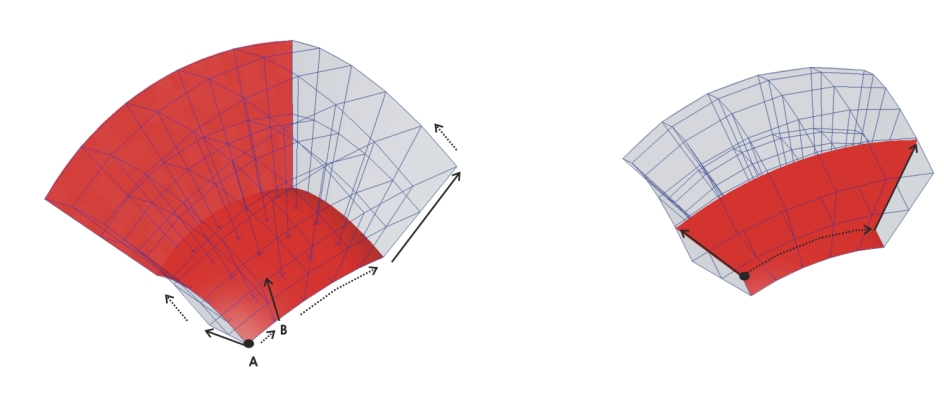
\includegraphics[width=0.75\paperwidth]{graphics/c_fig3.jpg}}]~
\end{description}
\caption{\label{fig:Global-Node-Numbering.}Global Node Numbering. Left: Global
node numbering starts at the base of arrow A (theta\_min, fi\_min,
radius\_inner), and advances from 1 at the base to \emph{nodez} at
the tip. Upon reaching the tip, numbering continues from the base
of arrow B (\emph{nodez}+1) to its tip (2 \emph{nodez}), and so on
for all nodes on the plane fi = fi\_min. Right: After completing each
theta radius plane, the fi index is incremented and numbering commences
from (theta\_min, radius\_inner) as on the left.}
\end{figure}

\par\end{center}

For a global mesh, CitcomS is also capable of generating a mesh for
an entire spherical shell in which elements in map view are approximately
equal in area. In the full spherical mode, CitcomS has 12 caps numbered
0 to 11 (Figure \ref{fig:Topological-connectivity-of}). 

\noindent \begin{center}
\begin{figure}[H]
\noindent \begin{centering}
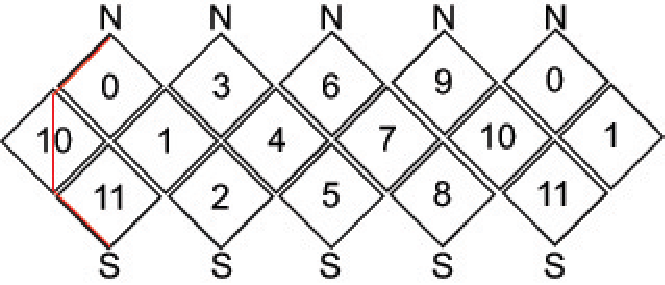
\includegraphics{graphics/cap_order.pdf}
\par\end{centering}

\caption{\label{fig:Topological-connectivity-of}Topological connectivity of
the 12 caps. N is the north pole and S is the south pole. The red
line marks the 0 degree meridian.}
\end{figure}

\par\end{center}

The caps are approximately square in map view so that the edges of
the square are oriented diagonally with respect to latitude and longitude.
The four corners of the domain are connected by great circles (Figure
\ref{fig:Orthographic-projection-of}). One would normally associate
at least one processor with one cap. However, CitcomS can further
decompose the domain such that additional processors are used to divide
caps uniformly along the two edges of the caps (Figure \ref{fig:Orthographic-projection-of})
as well as in radius. 

\noindent \begin{center}
\begin{figure}[H]
\noindent \begin{centering}
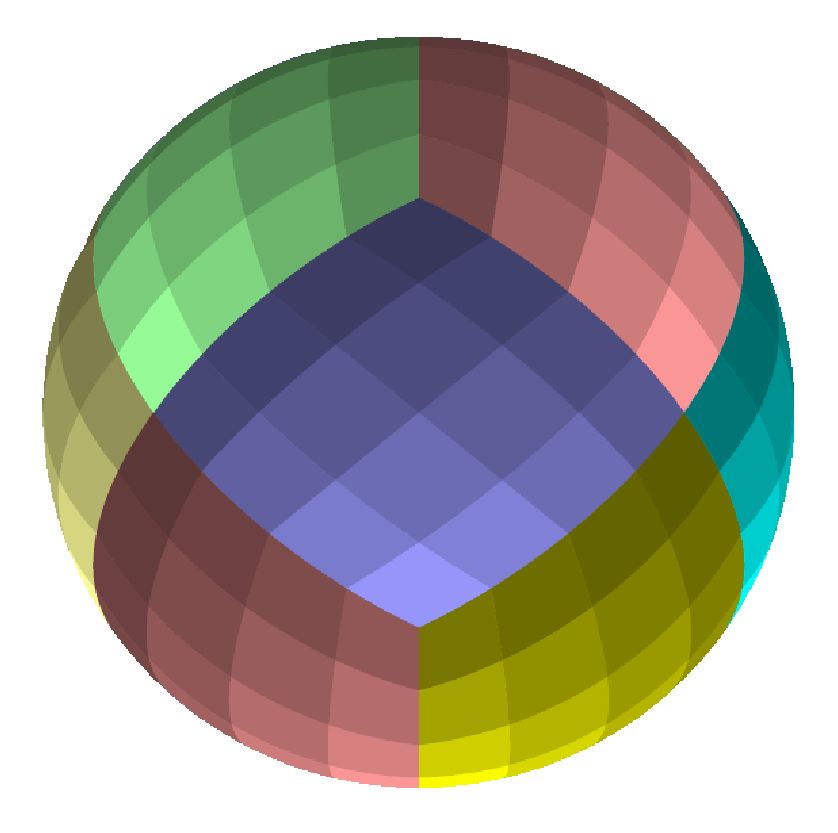
\includegraphics[scale=0.75]{graphics/proc_mesh.eps}
\par\end{centering}

\caption{\label{fig:Orthographic-projection-of}Orthographic projection of
processors from a full CitcomS mesh in which there are 16 processors
in map view for each cap. The CitcomS cap is shown as distinct colors
while the processor domains within the caps are indicated by the intensity
of the color. This example was produced for a run with 2 processors
in radius such that the total number of processors was 12$\times$16$\times$2=384.}
\end{figure}

\par\end{center}


\chapter{Installation and Getting Help}


\section{Introduction}

CitcomS has been tested on Linux, Mac OS X, Sun Solaris and several
NSF TeraGrid platforms. You should have no trouble installing CitcomS
on most Unix-like systems. 

Most users will install CitcomS from the released source package.
The following sections will lead you through the installation process.
Advanced users and software developers may be interested in downloading
the latest CitcomS source code directly from the CIG source code repository,
instead of using the prepared source package; see Section \ref{sec:Software-Repository}
later in this chapter.


\section{Getting Help}

For help, send e-mail to the CIG Mantle Convection Mailing List \url{cig-mc@geodynamics.org}.
You can subscribe to the Mailing List and view archived discussion
at the Geodynamics Mail Lists web page \url{geodynamics.org/cig/lists}.


\section{System Requirements}

Installation of CitcomS requires the following:
\begin{itemize}
\item A C compiler
\item An MPI library
\item If using Pyre: between Python 2.4 to 2.6, including header files (Python.h),
and the pythia package (see below).
\end{itemize}
You can install all the dependencies in one command on most Linux
machines. On Debian, Ubuntu or similar distributions, use this command
(as \texttt{root}):
\begin{lyxcode}
\$~apt-get~install~build-essential~python-dev~\textbackslash{}~\\
~~~~~~~~~~openmpi-dev~openmpi-bin
\end{lyxcode}
On Red Hat, Fedora, CentOS, OpenSuSE or similar distributions, use
this command (as \texttt{root}):
\begin{lyxcode}
\$~yum~install~make~automake~gcc~gcc-c++~kernel-devel~\textbackslash{}~\\
~~~~~~python~python-devel~openmpi~openmpi-libs~openmpi-devel
\end{lyxcode}
On Mac OS X, Python is installed by default. You will need to install
a C compiler and MPI library (see sections below).

MPI installations are typically configured for a particular compiler,
and provide a special wrapper command to invoke the right compiler.
Therefore, the choice of MPI implementation often determines which
C compiler to use.
\begin{quote}
\textbf{Note:} Users familiar with older versions of CitcomS may prefer
to install only the legacy CitcomS tools, \texttt{CitcomSFull} and
\texttt{CitcomSRegional}, and forgo use of Python and the Pyre framework.
By default in CitcomS 3.2.0 this is how CitcomS is configured. This
process requires only a C compiler and an MPI library. For more information,
see Section \ref{sec:Installing-without-Pyre} later in this chapter.
\end{quote}
If you are going to use solver coupling, you will also need a decent
C++ compiler (e.g., g++ 3.2 or newer) and the Exchanger package; see
Section \ref{sec:Exchanger-Configuration-(Optional)}. Optionally,
CitcomS can be configured to use a parallel HDF5 library; see Section
\vref{sec:HDF5-Configuration}.


\subsection{C Compiler}

On Unix or Linux systems, there is a high likelihood that a usable
C compiler is already installed. To check, type \texttt{cc} at the
shell prompt:
\begin{lyxcode}
\$~cc

cc:~no~input~files

\$
\end{lyxcode}
On Linux, if the \texttt{cc} command is not found, install GCC using
the package manager for your distribution.

The Mac OS X version of GCC is included in a software development
suite called Xcode. Xcode is available as a free download at the Apple
Developer Connection \url{developer.apple.com}.
\begin{quote}
\textcolor{red}{Warning:} \textcolor{black}{If you are using an Intel
compiler on an Itanium CPU, do not use the} \texttt{\textcolor{black}{-O3}}
\textcolor{black}{optimization flag as reports indicate that this
optimization level will generate incorrect codes. For any compiler,
you should always be careful about the correctness of the compiled
codes when using an} \texttt{\textcolor{black}{-O3}} \textcolor{black}{or
higher optimization level.}
\end{quote}

\subsection{MPI Library}

CitcomS requires a library which implements the MPI standard (either
version 1 or 2). Several free, open-source implementations of MPI
are available.

A popular choice is MPICH \url{www-unix.mcs.anl.gov/mpi/mpich}. Other
choices include LAM/MPI \url{www.lam-mpi.org} and Open MPI \url{www.open-mpi.org}.
Installing MPI from source involves walking through the standard GNU
build procedure (\texttt{configure \&\& make \&\& make install}) while
logged in as \texttt{root}.

Linux users may have a prebuilt MPI package available for their distribution.
On Mac OS X, the Fink package manager offers a prepackaged version
of LAM/MPI \url{www.lam-mpi.org}; so if you have Fink \url{fink.sourceforge.net}
installed, simply enter the following command from a Terminal window
to install LAM/MPI:
\begin{lyxcode}
\$~fink~install~lammpi~lammpi-dev
\end{lyxcode}

\subsubsection{MPI C Compiler Command}

Once you have an MPI library installed, make sure its C complier command
is on your PATH. Unfortunately, the name of this command varies from
one MPI implementation to the next. The CitcomS configuration script
searches for the following MPI C command names:
\begin{lyxcode}
mpicc~hcc~mpcc~mpcc\_r~mpxlc~cmpicc
\end{lyxcode}

\subsection{Python (Optional)}

Your system may already have a suitable Python interpreter installed.
To check, type the \texttt{python} command:
\begin{lyxcode}
\$~python~-V

Python~2.5.2
\end{lyxcode}
Mac OS X 10.3 and later ships with a suitable version of Python preinstalled.
If you're using an older version of Mac OS X, or for more information
in general, see Python on the Mac \url{www.python.org/download/mac}
at the Python web site.

On Linux, simply install the binary system package available for your
distribution. Be sure to select the Python development package (typically
called \texttt{python-dev}) in addition to the core Python package
-- even if you don't plan on doing any Python software development.
The development package contains the Python header files (Python.h),
which are necessary for building CitcomS.

If you are working on a cluster and \texttt{python} is too old, try
poking around a little. Sometimes multiple versions of Python are
installed on the same system:
\begin{lyxcode}
\$~python~-V

Python~2.2.3

\$~which~python

/usr/bin/python

\$~ls~/usr/bin/python{*}

/usr/bin/python~/usr/bin/python2~/usr/bin/python2.2

/usr/bin/python24~/usr/bin/python2.4

\$
\end{lyxcode}
In the above scenario, it is useful to create an alias to the newer
Python:
\begin{lyxcode}
\$~cd~\textasciitilde{}/bin

\$~ln~-s~/usr/bin/python2.4~python

\$~export~PATH=\$HOME/bin:\$PATH

\$~cd

\$~hash~-r

\$~which~python

\textasciitilde{}/bin/python

\$~python~-V

Python~2.4.1

\$
\end{lyxcode}
If absolutely necessary, one can easily build Python from source using
a C compiler. You can download Python from the Python website \url{www.python.org}.
Please note that Pyre in CitcomS does not work with Python 2.7 or
higher.


\subsection{Pythia (Optional)}

The current version of pythia package can be downloaded from the \href{http://www.geodynamics.org/cig/software/pythia}{CIG Pythia page}.


\section{Downloading and Unpacking Source}

To obtain CitcomS, go to the Geodynamics Software Packages web page
\url{geodynamics.org/cig/software/packages/mc/citcoms}, download
the source archive and unpack it using the \texttt{tar} command: 
\begin{lyxcode}
\$~tar~xzf~CitcomS-3.2.0.tar.gz
\end{lyxcode}

If you don't have GNU Tar, try the following command instead: 
\begin{lyxcode}
\$~gunzip~-c~CitcomS-3.2.0.tar.gz~|~tar~xf~-
\end{lyxcode}

\section{Installation Procedure}

After unpacking the source, use the following procedure to install
CitcomS:
\begin{enumerate}
\item Navigate (i.e., \texttt{cd}) to the directory containing the CitcomS
source\texttt{.}~\\
\texttt{}~\\
\texttt{\$ cd CitcomS-3.2.0}
\item Type .\texttt{/configure} to configure the package for your system\texttt{.}~\\
\texttt{}~\\
\texttt{\$ ./configure}
\item Type \texttt{make} to build the package.\texttt{}~\\
\texttt{}~\\
\texttt{\$ make}
\end{enumerate}
If you are content to run CitcomS from the build directory, then you
are done. Upon successful completion, the \texttt{make} command creates
a script called \texttt{citcoms} in the \texttt{bin} subdirectory;
this is the script you will use to run CitcomS. You may wish to add
the \texttt{bin} directory to your \texttt{PATH}.

For more details about \texttt{configure}, see Section \ref{sec:Configuration}
below.


\subsection{Installing to a Secondary Location (Optional)}

Optionally, after building CitcomS, you can install it in a secondary
location using the \texttt{make install} command. This is not necessary
for using CitcomS and is not recommended for most situations. It is
documented only for the sake of completeness.

By default, CitcomS is configured to install under \texttt{/usr/local},
which is not writable by normal users. To install as an ordinary user,
give \texttt{make install} the \texttt{prefix} option, specifying
a directory to which you have write access:
\begin{lyxcode}
\$~make~install~prefix=\$HOME/cig
\end{lyxcode}
The above command will install CitcomS under \texttt{\$HOME/cig}.
Afterwards, you may wish to add \texttt{PREFIX/bin} (\texttt{\$HOME/cig/bin},
in this example) to your \texttt{PATH}.

After running \texttt{make install}, you may (if desired) run \texttt{make
clean} in the build directory to save disk space. You are also free
to delete the source/build directory altogether. (Note that \texttt{make
install} installs the examples under \texttt{PREFIX/share/CitcomS/examples}.)


\section{\label{sec:Configuration}Configuration}

The \texttt{configure} script checks for various system features.
As it runs, it prints messages informing you of which features it
is checking for. Upon successful completion, it generates a \texttt{Makefile}
in each source directory of the package. It also generates a \texttt{config.h}
header file, which contains system-dependent definitions. 

The \texttt{configure} script will attempt to guess the correct values
of various installation parameters. In the event that the default
values used by \texttt{configure} are incorrect for your system, or
\texttt{configure} is unable to guess the value of a certain parameter,
you may have to specify the correct value by hand.
\begin{quote}
\textbf{Important:} If the \texttt{configure} script fails, and you
don't know what went wrong, examine the log file \texttt{config.log}.
This file contains a detailed transcript of all the checks \texttt{configure}
performed. More importantly, it includes the error output (if any)
from your compiler. When seeking help for \texttt{configure} failures
on the CIG Mantle Convection Mailing List \url{cig-mc@geodynamics.org},
please send \texttt{config.log} as an attachment.
\end{quote}
Upon successful completion, \texttt{configure} will print a brief
configuration summary.

If Pyre is enabled, the \texttt{configure} script will automatically
check for needed Python dependencies, including the Pythia package
(which includes the Pyre framework). If necessary, \texttt{configure}
will download missing Python packages from the Internet and store
them under \texttt{\textit{\emph{deps/}}}. These are Python packages
which are required (either directly or indirectly) by CitcomS.


\subsection{Configure Usage}

For a detailed list of \texttt{configure} variables and options, give
\texttt{configure} the \texttt{-{}-help} option:
\begin{lyxcode}
\$~./configure~-{}-help
\end{lyxcode}
The following is a summary of the variables and options that are important
when installing CitcomS. 


\subsection{Environment Variables}

Environment variables may be specified as arguments to \texttt{configure},
e.g.,
\begin{lyxcode}
\$~./configure~CC=icc~\#~use~the~Intel~compiler
\end{lyxcode}
\noindent \begin{center}
\begin{table}[H]
\noindent \centering{}%
\begin{tabular}{|>{\centering}p{1in}|>{\raggedright}p{3.5in}|}
\hline 
\textbf{Variable} & \textbf{Description}\tabularnewline
\hline 
\hline 
PYTHON & Python interpreter. This is useful if you have Python installed in
a non-standard location, e.g.,

\texttt{~~./configure \textbackslash{}}

\texttt{~~~~~~PYTHON=/opt/python2.5/bin/python} 

By default, \texttt{configure} will search for a suitable Python interpreter
using your \texttt{PATH} environment variable.\tabularnewline
\hline 
CC & C compiler command. This is usually set to the name of an MPI wrapper
command, e.g.,

\texttt{~~./configure \textbackslash{}}

\texttt{~~~~~~CC=/opt/mpich-1.2.6/bin/mpicc}

See Section \vref{sec:MPI-Configuration} for details and examples.\tabularnewline
\hline 
CFLAGS & C compiler flags. This can be set for optimization flags.\tabularnewline
\hline 
CPPFLAGS & C preprocessor flags; e.g., \texttt{-I<dir>} if you have headers in
a nonstandard directory.\tabularnewline
\hline 
LDFLAGS & Linker flags; e.g., \texttt{-L<dir>} if you have libraries in a nonstandard
directory.\tabularnewline
\hline 
LIBS & Library flags; e.g., -l<lib> if additional library is needed\tabularnewline
\hline 
\end{tabular}
\end{table}

\par\end{center}


\subsection{\label{sec:MPI-Configuration}MPI Configuration}

By default, \texttt{configure} will search for a C compiler using
your \texttt{PATH} environment variable. It prefers MPI wrapper commands
(such as \texttt{mpicc}) to ordinary compiler commands (such as \texttt{cc}
or \texttt{gcc}). You may specify the compiler command name manually
using the \texttt{CC} variable:
\begin{lyxcode}
\$~./configure~CC=/opt/mpich-1.2.6/bin/mpicc
\end{lyxcode}
The \texttt{configure} script will test for the presence of the MPI
header (\texttt{mpi.h}) and an MPI library using the C compiler command.
If \texttt{CC} is set to an MPI wrapper command such as \texttt{mpicc},
and/or the MPI header and library files are installed in a standard
location (i.e., \texttt{/usr/include} and \texttt{/usr/lib}), these
\texttt{configure} tests should succeed without difficulty.

But if CC is set to an ordinary compiler command name (e.g., \texttt{cc}
or \texttt{gcc}) and MPI is installed in a non-standard location,
you must manually specify \texttt{CPPFLAGS} and \texttt{LDFLAGS},
so that the compiler can find the MPI header files and libraries.


\subsubsection{Manually Specifying MPI \texttt{include} and \texttt{lib} Directories}
\begin{lyxcode}
\$~./configure~\textbackslash{}

CPPFLAGS=\textquotedbl{}-I/opt/mpich-1.2.6/include\textquotedbl{}~\textbackslash{}

LDFLAGS=\textquotedbl{}-L/opt/mpich-1.2.6/lib~-lmpich\textquotedbl{}
\end{lyxcode}

\subsubsection{Manually Specifying MPI \texttt{include} and \texttt{lib} Directories
and an Alternative Compiler}
\begin{lyxcode}
\$~./configure~\textbackslash{}

CC=icc~\textbackslash{}

CPPFLAGS=\textquotedbl{}-I/opt/mpich-1.2.6/include\textquotedbl{}~\textbackslash{}

LDFLAGS=\textquotedbl{}-L/opt/mpich-1.2.6/lib~-lmpich\textquotedbl{}
\end{lyxcode}
Note that it may be necessary to specify the name of the MPI library
itself in \texttt{LDFLAGS} using the \texttt{-l} compiler option.
If a library name is not given -- or if the given option doesn't work
-- \texttt{configure} will automatically try linking using \texttt{-lmpi}
and, if that fails, \texttt{-lmpich}.


\section{\label{sec:Exchanger-Configuration-(Optional)}Exchanger Configuration
(Optional)}

This version of CitcomS is capable of solver coupling. Two or more
instances of CitcomS solvers can be coupled together to solve a problem
with different length and time scales \cite{Tan et al GeoFramework Part I}.
An external Exchanger package is needed for solver coupling. You can
download Exchanger at CIG's Exchanger web page \url{geodynamics.org/cig/software/packages/cs/exchanger}.
After you download and untar the package, you can configure and install
Exchanger using these commands:
\begin{lyxcode}
\$~cd~Exchanger-1.0.1/

\$~./configure~-{}-prefix=\$HOME/cig

\$~make

\$~make~install
\end{lyxcode}
By default, CitcomS will attempt to auto-detect your Exchanger installation
and will disable Exchanger support if it is not found. You may specify
the location of your Exchanger installation by setting the PYTHONPATH
environment variable to the appropriate installation prefix.
\begin{lyxcode}
\$~cd~CitcomS-3.2.0/

\$~export~PYTHONPATH=\$HOME/cig/lib/python2.5/site-packages:\$PYTHONPATH

\$~./configure~-{}-with-exchanger
\end{lyxcode}

\section{\label{sec:HDF5-Configuration}HDF5 Configuration (Optional)}

For writing its output in binary format, CitcomS requires parallel
HDF5 (PHDF5). In turn, PHDF5 requires an MPI library with MPI-IO support
and a parallel file system. If an existing installation of the PHDF5
library is not available on your cluster, you can compile it from
source by following the instructions in the file \texttt{\small{release\_docs/INSTALL\_parallel}}
under the HDF5 source tree. Under Debian Linux, you may simply install
the \texttt{libhdf5-mpich}, \texttt{libhdf5-mpich-dev} and \texttt{hdf5-tools}
packages.
\begin{quote}
\textbf{NOTE:} Most post-processing and visualization scripts discussed
in Chapter \ref{cha:Postprocessing-and-Graphics} only understand
ASCII output. An additional step to convert the HDF5 output files
to ASCII files in necessary before using those scripts.
\end{quote}
By default, CitcomS will attempt to auto-detect your PHDF5 installation,
and will disable HDF5 support if it is not found. You may specify
the location of your PHDF5 installation by setting the PHDF5\_HOME
environment variable to the appropriate installation prefix.
\begin{lyxcode}
\$~export~PHDF5\_HOME=/opt/phdf5/1.6.5

\$~./configure~-{}-with-hdf5
\end{lyxcode}

\subsection{Additional Tools}

While the following software is not necessary for the normal operation
of CitcomS, you may find it useful for accessing CitcomS data in HDF5
files.


\subsubsection{NumPy}

NumPy is an extension to Python which adds support for multi-dimensional
arrays for use in scientific computing. You may download NumPy from
the NumPy home page \url{numpy.scipy.org}. To compile and install
this extension, download it and issue the following commands after
extracting it:
\begin{lyxcode}
\$~cd~numpy-1.0

\$~python~setup.py~install~-{}-prefix=\$HOME/cig
\end{lyxcode}
Alternatively, under Debian Linux you can install the \texttt{python-numpy}
package. On Gentoo Linux, NumPy is available in the \texttt{dev-python/numpy}
ebuild.


\subsubsection{\label{sub:PyTables}PyTables}

PyTables is an extension to Python and can expose HDF5 array datasets
as Python NumPy arrays. It is available at PyTables \url{www.pytables.org}.

To compile and install this extension, download the latest stable
version and issue the following commands:
\begin{lyxcode}
\$~cd~pytables-1.3.3

\$~python~setup.py~install~-{}-prefix=\$HOME/cig
\end{lyxcode}
To install on Debian Linux, you may use the \texttt{python-tables}
package instead. On Gentoo Linux, it is available in the \texttt{dev-python/pytables}
ebuild.


\subsubsection{HDFView}

HDFView is a visual tool written in Java for browsing and editing
HDF5 files. You may download it from the HDFView home page \url{hdf.ncsa.uiuc.edu/hdf-java-html/hdfview}.


\subsubsection{\label{sub:OpenDXutils}OpenDXutils}

In order to import HDF5 files into OpenDX, you need the OpenDXutils
package from the Cactus project. Go to the OpenDXutils package website
\url{www.cactuscode.org/Visualization/openDX} and follow the instructions
to download and install the package. Note that you will need to set
both \texttt{DXMODULES} and \texttt{DXMDF} environment variables before
running OpenDX to load the package.


\section{GGRD Configuration (Optional)}

CitcomS can read data from files for initial temperature, boundary
conditions, material control and others. By default, these files are
in ASCII format, and the data in the files must be ordered in the
same way of the node ordering. As a result, whenever the mesh is changed,
these data files need to be regenerated to satisfy the ordering requirement.
This restriction can be lifted if using GRD data files. GRD files
are binary files in NetCDF format (Network Common Data Form). GRD
files are widely used in GMT (Generic Mapping Tools) as well.

The GRD file support can be enabled at configuration time. It requires
the installation of HC package \url{geodynamics.org/cig/software/packages/mc/hc},
a 1D global mantle circulation solver which can compute velocities,
tractions, and geoid for simple density distributions and plate velocities.
To install HC, you will also need the GMT and NetCDF packages (library
and header files). See the \texttt{README.TXT} file in HC for instructions
on installation. After HC is installed, note the directory (for example:
\texttt{\$HOME/cig/HC-1\_0}) of HC installation, and execute these
commands:
\begin{lyxcode}
\$~export~HC\_HOME=\$HOME/cig/HC-1\_0

\$~./configure~-{}-with-ggrd
\end{lyxcode}
You may need to set \texttt{GMTHOME} and \texttt{NETCDFHOME} environment
variables if these packages is not installed in the system directory.


\section{\label{sec:Batch-System-Configuration}Batch System Configuration}

If you are installing CitcomS on a cluster with a batch system, you
can configure Pyre such that the \texttt{citcoms} command automatically
submits jobs to the batch queue. Pyre contains support for the LSF,
PBS, and Globus batch systems.

The command to submit a batch job depends upon the particular batch
system used. Further, the command used in a batch script to launch
an MPI program varies from one cluster to the next. This command can
vary between two clusters, even if the clusters use the same batch
system! On some systems, \texttt{mpirun} is invoked directly from
the batch script. On others, a special wrapper is used instead. If
you need help to configure Pyre for your cluster, you can contact
CIG Mantle Convection Mailing List \url{cig-mc@geodynamics.org} for
assistance.

Properly configured, Pyre can handle job submissions automatically,
insulating users from the details of the batch system and the site
configuration. This feature has the most value when the system administrator
installs a global Pyre configuration file on the cluster (under \texttt{/etc/pythia-0.8}),
for the benefit of all users and all Pyre-based applications.

For more information on configuring Pyre for your batch system, see
CIG's Pythia page \url{geodynamics.org/cig/software/packages/cs/pythia/docs/batch}.
For more information on batch system configuration as it pertains
to running CitcomS, see Section \vref{sub:Launchers-and-Schedulers}.


\section{\label{sec:Installing-without-Pyre}Installing with Pyre}

By default, CitcomS 3.2.0 does not install using Pyre. To build CitcomS
binaries with the Pyre wrappers (necessary for the example Cookbooks),
call \texttt{configure} using the \texttt{-{}-with-pyre} option:
\begin{lyxcode}
\$~./configure~-{}-with-pyre=yes
\end{lyxcode}
The only system requirements for this configuration are an MPI library
and a C compiler. With Pyre the make command will build \texttt{pycitcoms}
and \texttt{mpipycitcoms} as well as the script \texttt{citcoms} used
for running CitcomS. Without Pyre the \texttt{make} command will build
two command-line tools, \texttt{CitcomSFull} and \texttt{CitcomSRegional},
for running the full solver and the regional solver, respectively.


\section{\label{sec:Software-Repository}Installing from the Software Repository}

The CitcomS source code is available via a Subversion server at the
Geodynamics website \url{geodynamics.org}. This allows users to view
the revision history of the code and check out the most recent development
version of the software.
\begin{quote}
\textbf{NOTE:} If you are content with the prepared source package,
you may skip this section.
\end{quote}

\subsection{Tools You Will Need}

In addition to the usual system requirements, you will need a handful
of additional development tools installed in order to work with the
source from the CIG software repository.

First, you must have a Subversion client installed. To check, type
\texttt{svn}; it should return a usage message.
\begin{lyxcode}
\$~svn

Type~'svn~help'~for~usage.
\end{lyxcode}
For more information on Subversion, visit the Subversion website \url{subversion.tigris.org}.

Second, you must have the GNU tools Autoconf, Automake, and Libtool
installed. To check, enter the following commands:
\begin{lyxcode}
\$~autoconf~-{}-version

\$~automake~-{}-version

\$~libtoolize~-{}-version
\end{lyxcode}
For more information about these GNU tools, see the GNU website \url{www.gnu.org/software}.
The CitcomS v3.2.0 source package was created with Autoconf 2.68,
Automake 1.11.2, and Libtool 2.4.2.


\subsection{Download Source from Subversion}

To check out the latest version of the software, use the \texttt{svn
checkout} command:
\begin{lyxcode}
\$~svn~checkout~http://geodynamics.org/svn/cig/mc/3D/CitcomS/trunk~CitcomS
\end{lyxcode}
This will create the local directory \texttt{CitcomS} (if it doesn't
already exist) and fill it with the latest CitcomS source from the
CIG software repository.

The \texttt{CitcomS} directory thus created is called a \emph{working
copy}. To merge the latest changes into an existing working copy,
use the \texttt{svn update} command:
\begin{lyxcode}
\$~cd~CitcomS

\$~svn~update
\end{lyxcode}
This will preserve any local changes you have made to your working
copy.


\subsection{Generating the GNU Build System}

Your working directory should now contain a fresh checkout of CitcomS:
\begin{lyxcode}
\$~ls

CitcomS

\$
\end{lyxcode}
Before you can run \texttt{configure} or \texttt{make}, you must generate
the necessary files using the GNU tools. The easiest way to do this
is to run \texttt{autoreconf -i}:
\begin{lyxcode}
\$~cd~CitcomS

\$~autoreconf~-i

\$~./configure

\$~make
\end{lyxcode}
The \texttt{autoreconf} tool runs Autoconf to generate the \texttt{configure}
script from \texttt{configure.ac}. It also runs Automake to generate
\texttt{Makefile.in} from \texttt{Makefile.am} in each source directory.

The configure script stores dependency information for source files
in hidden subdirectories called \texttt{.deps}. If source files are
added, deleted, moved, or renamed -- which may happen if you run \texttt{svn
update} to merge the latest changes -- the \texttt{make} command may
report errors for source files which no longer exist. If this happens,
clean your existing configuration using the \texttt{make distclean}
command, and then re-run \texttt{configure} and \texttt{make}:
\begin{lyxcode}
\$~make~distclean

\$~./configure

\$~make
\end{lyxcode}
The \texttt{make} \texttt{distclean} command deletes all files generated
by \texttt{configure}, including the Makefiles themselves! Therefore,
after running \texttt{make} \texttt{distclean}, you will not be able
to run \texttt{make} again until you re-run \texttt{configure}.


\chapter{Running CitcomS}


\section{Using CitcomS without Pyre}

Regardless of whether you build CitcomS with or without Pyre, two
binary executables, \texttt{CitcomSRegional} and \texttt{CitcomSFull},
are always placed under the \texttt{bin} directory. These programs
are compiled from pure C code and do not use Python or the Pyre framework.
Each program has the same usage:
\begin{lyxcode}
\$~mpirun~{[}mpi\_options{]}~CitcomSRegional~inputfile~\\
\$~mpirun~{[}mpi\_options{]}~CitcomSFull~inputfile
\end{lyxcode}
Two input file examples, one for a regional spherical model and one
for a full spherical model, are provided in the \texttt{examples/Regional}
and \texttt{examples/Full} directories, respectively. The meaning
of the input parameters is described in Appendix \vref{cha:Appendix-A:-Input}.

The pure C version, compared to the Pyre version, shares the same
input parameters and functionality, but is less flexible in changing
parameters and in launching parallel jobs. Users are encouraged to
use the Pyre version if possible. In the following sections and Chapter
\ref{cha:Cookbooks}, we will concentrate on the Pyre version only.


\section{Using CitcomS with Pyre}

If you build CitcomS with the Pyre framework, an additional executable,
\texttt{citcoms}, is placed under the \texttt{bin} directory. The
\texttt{citcoms} executable is a Python script used for running both
the regional and full spherical models using Pyre. Executed without
any command line options, \texttt{citcoms} will run a regional model
with default parameters. It can also run a full spherical model if
the correct parameters are set (see Section \vref{sec:Cookbook-1:-Global}
for an example).

On input, CitcomS needs numerous parameters to be specified (see Appendix
\ref{cha:Appendix-A:-Input} for a full list). All parameters have
sensible default values. Since you will likely want to specify the
parameters of your CitcomS runs, you will need to alter both computational
details (such as the number of time steps) and controlling parameters
specific to your problem (such as the Rayleigh number). These input
parameters, or properties in the Pyre terminology, are grouped under
several Pyre components.

Most of the properties you will set using CitcomS have names which
are identical to the parameters for CitcomS in pure C version, which
are described in Appendix \ref{cha:Appendix-A:-Input}.


\section{Changing Parameters }

There are several methods to set the input parameters for CitcomS:
via the command line, or by using a configuration file in \texttt{.cfg}
format.


\subsection{Using the Command Line}

Pyre uses the following syntax to change properties from the command
line. To change the value of a property of a component, use:
\begin{lyxcode}
-{}-{[}component{]}.{[}property{]}={[}value{]}
\end{lyxcode}
Each component is attached to a facility, so the option above can
also be written as: 
\begin{lyxcode}
-{}-{[}facility{]}.{[}property{]}={[}value{]}
\end{lyxcode}
Each facility has a default component attached to it. A different
component can be attached to a facility by:
\begin{lyxcode}
-{}-{[}facility{]}={[}new\_component{]}~
\end{lyxcode}

\subsection{Using a \texttt{.cfg} File}

Entering all those parameters via the command line involves the risk
of typographical errors, which can lead to undesired results. You
may find it easier to write a brief \texttt{.cfg} input file that
contains the parameters. This file has a format similar to a Windows
INI file. The file is composed of one or more sections which are formatted
as follows:
\begin{lyxcode}
{[}CitcomS.component1.component2{]}~\\
\#~this~is~a~comment~\\
property1~=~value1~\\
property2~=~value2~~;~this~is~another~comment
\end{lyxcode}
We strongly recommend that you use \texttt{.cfg} files for your work.
The files are syntax-colored by the \texttt{vim} editor. (Upon termination
of each run, all of the parameters are logged in a \texttt{.cfg} file.)


\subsection{Using a \texttt{.pml} File}

A \texttt{.pml} file is an XML file that specifies parameter values
in a highly structured format. XML files are intended to be read and
written by machines, not edited manually by humans. The \texttt{.pml}
file format is intended for applications in which CitcomS input files
are generated by another program, e.g., a GUI, web application, or
a high-level structured editor. This file fomat will not be discussed
or used further in the manual. It is composed of nested sections which
are formatted as follows:
\begin{lyxcode}
<component~name='component1'>~\\
~~~~<component~name='component2'>~\\
~~~~~~~~<property~name='property1'>value1</property>~\\
~~~~~~~~<property~name='property2'>value2</property>~\\
~~~~</component>~\\
</component>
\end{lyxcode}

\subsection{Specification and Placement of Configuration Files}

One or more configuration files and command line options may be specified
on the command line:
\begin{lyxcode}
\$~citcoms~a.cfg~b.cfg~-{}-foo.bar=baz
\end{lyxcode}
In addition, the Pyre framework searches for configuration files named
\texttt{CitcomS.cfg} in several predefined locations. You may put
settings in any or all of these locations, depending on the scope
you want the settings to have:
\begin{enumerate}
\item \texttt{PREFIX/etc/CitcomS.cfg}, for system-wide settings;
\item \texttt{\$HOME/.pyre/CitcomS/CitcomS.cfg}, for user settings and preferences;
\item the current directory (\texttt{./CitcomS.cfg}), for local overrides. 
\end{enumerate}
Parameters given directly on the command line will override any input
contained in a configuration file. If more than one configuration
files are given on the command line, the later one overrides the former
ones. Configuration files given on the command line override all other
\texttt{CitcomS.cfg} files. The \texttt{CitcomS.cfg} files placed
in (3) will override those in (2), (2) overrides (1), and (1) overrides
only the built-in defaults.


\section{Uniprocessor Example}

CitcomS runs similarly in full spherical or regional modes. For the
purpose of this example, you will perform a test run of the regional
version on a workstation. Execute the following on the command line:
\begin{lyxcode}
\$~citcoms~-{}-steps=10~-{}-controller.monitoringFrequency=5~\textbackslash{}~\\
-{}-solver.datafile=example0~-{}-solver.mesher.nodex=17~-{}-solver.mesher.nodey=17
\end{lyxcode}
This runs a default convection problem in a regional domain for 10
time steps and with a mesh of 17 $\times$ 17 $\times$ 9 nodal points.
Since we did not provide the parameter \texttt{solver.mesher.nodez},
the default value 9 is used. The model results are written to files
\texttt{example0.{*}} with an interval of 5 time steps. 

Instead of writing the input parameters on the command line, you can
put them in a \texttt{.cfg} file. The CitcomS source package contains
an \texttt{examples} directory (the \texttt{make install} command
installs the examples under \texttt{PREFIX/share/CitcomS/examples},
where \texttt{PREFIX} is the \texttt{CitcomS} installation directory).
In this directory, you will find a configuration file equivalent to
the previous example: \texttt{example0.cfg}. You can run the model
using:
\begin{lyxcode}
\$~citcoms~example0.cfg
\end{lyxcode}

\subsubsection{Example: Uniprocessor, \texttt{example0.cfg}}
\begin{lyxcode}
{[}CitcomS{]}~\\
steps~=~5~\\
~\\
{[}CitcomS.controller{]}~\\
monitoringFrequency~=~1~\\
~\\
{[}CitcomS.solver{]}~\\
datafile~=~example0~\\
~\\
{[}CitcomS.solver.mesher{]}~\\
nodex~=~~17~\\
nodey~=~~17
\end{lyxcode}

\section{\label{sec:Multiprocessor-Example}Multiprocessor Example}

In order to run this example, you should be on a Beowulf cluster with
four or more processors, or on a supercomputer; and you should be
in the directory in which the input file is located, in this case,
the \texttt{examples} directory. CitcomS has been extensively used
on both environments, using up to several hundred processors. How
to run a multiprocessor CitcomS model depends on your hardware and
software settings, e.g., whether a batch system is used, what the
names of the computers in a cluster are, and how the file system is
organized. This section will lead you through the different settings
of a parallel environment. 


\subsubsection{Example: Multiprocessor, \texttt{example1.cfg }}
\begin{lyxcode}
{[}CitcomS{]}~\\
steps~=~70~\\
~\\
{[}CitcomS.controller{]}~\\
monitoringFrequency~=~10~\\
~\\
{[}CitcomS.solver{]}~\\
datafile~=~example1~\\
~\\
{[}CitcomS.solver.mesher{]}~\\
nprocx~=~~2~\\
nprocy~=~~2~\\
nodex~~=~17~\\
nodey~~=~17~\\
nodez~~=~~9~~~~~~~~~~~~~~~~~~~~~~~~~~~~~~~~~~~~~~~~~~~~~~~~~~~~~~~~~~~~~~~~~~~~~~~~~~~~~~~~
\end{lyxcode}
This example uses 2 processors in colatitude ($x$-coordinate), 2
in longitude ($y$-direction), and 1 in the radial ($z$-direction),
i.e., it uses 4 processors in total. In addition, there will be 17
nodes in $x$ (theta), 17 nodes in $y$ (fi), and 9 nodes in $z$
(radius\_inner). The model will run for 70 time steps and the code
will output the results every 10 time steps.

It is important to realize that within the example script (and in
finite element method, FEM) the term ``node'' refers to the mesh points
defining the corners of the elements. In \texttt{example1.cfg}, this
is indicated with:
\begin{lyxcode}
nodex~~=~17~\\
nodey~~=~17~\\
nodez~~=~~9~
\end{lyxcode}
These quantities refer to the total number of FEM nodes in a given
direction for the complete problem, and for the example it works out
that within a given processor there will be 9 $\times$ 9 $\times$
9 nodes. Note that in the $x$-direction (or $y$) that for the entire
problem there are 17 nodes and there is one node shared between two
processors. This shared node is duplicated in two adjacent processors.
Unfortunately, ``nodes'' sometimes also refer to the individual computers
which make up a Beowulf cluster or supercomputer. In the example scripts,
this is indicated with:
\begin{lyxcode}
nprocx~=~~2~\\
nprocy~=~~2
\end{lyxcode}
\begin{figure}[H]
\begin{centering}
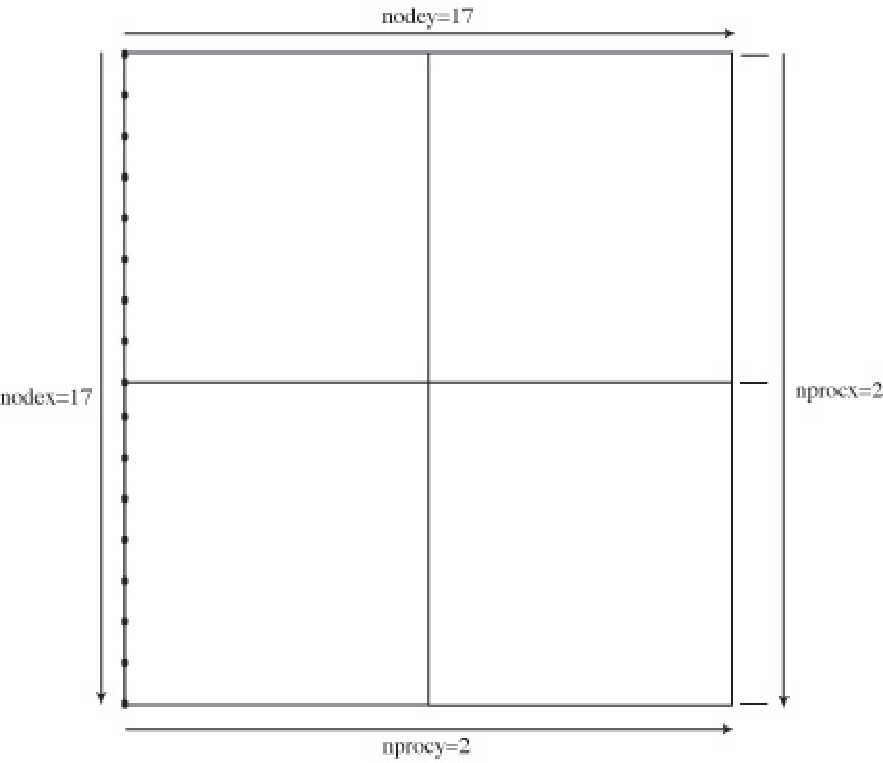
\includegraphics[width=0.5\paperwidth]{graphics/cookbook2.pdf}
\par\end{centering}

\caption{Computational Domain. Map view on the configuration of the top layer
of the computational nodes and the processors.}
\end{figure}



\subsection{Output Directories and Output Formats}

CitcomS potentially generates a large number of ASCII files. This
means that you will have to organize your directories carefully when
running CitcomS so that you can manage these files as well as use
a post-processing program contained in this distribution. 

How to best manage this large output depends on whether you will use
a local file system or a parallel file system. For example, if you
have a local hard disk on every machine (node) on a Beowulf cluster,
with each hard disk mounted locally to the machine, this scenario
is referred to as a local file system in this section. Or you might
use some kind of parallel file system on your computer (e.g., NFS,
GPFS, PVFS, to name a few), which is mounted on all of the nodes.
Usually your home directory is mounted on the parallel file system.
The local file system is usually more cost- and time-efficient than
the parallel file system. 

If you want CitcomS to write its output to the local hard disks, you
need to have a common directory structure on all of the local hard
disks. For example, if the directory \texttt{/scratch} exists on all
local hard disks, you can run the example script with:
\begin{lyxcode}
\$~citcoms~example1.cfg~-{}-solver.datadir=/scratch
\end{lyxcode}
The additional command line option will override the \texttt{datadir}
property, which specifies the output directory. The output files are
then placed in \texttt{/scratch} on each individual machine with a
filename prefix \texttt{example1.}

However, if the output directory name on each local hard disk depends
on the machine hostname, you can run the example script with:
\begin{lyxcode}
\$~citcoms~example1.cfg~-{}-solver.datadir=/scratch\_\%HOSTNAME
\end{lyxcode}
The special string \texttt{\%HOSTNAME} will be substituted by the
hostname of each machine. 

As the final example for a local file system, you can specify an arbitrary
output directory for each machine. To do so, you must write a program
to be executed on each machine which will print the output directory.
The program must be named \texttt{citcoms\_datadir} and must reside
on your path. An example of \texttt{citcoms\_datadir} can be found
in the \texttt{visual/} directory. Then you can run the example script
with:
\begin{lyxcode}
\$~citcoms~example1.cfg~-{}-solver.datadir=\%DATADIR
\end{lyxcode}
The special string \texttt{\%DATADIR} will be substituted by the output
of \texttt{citcoms\_datadir} for each machine.

If you want CitcomS to write its output to a parallel file system,
you have several choices. You can run the example script as follows
(substitute \texttt{\emph{username}} with your own username):
\begin{lyxcode}
\$~citcoms~example1.cfg~-{}-solver.datadir=/home/\emph{username}
\end{lyxcode}
The output files are then placed in your home directory with a filename
prefix \texttt{example1}. A potential problem with this approach is
that the directory \texttt{/home/}\texttt{\emph{username}} will be
flooded with hundreds of files, perhaps even tens of thousands of
files if you are running a model using several tens of processors
for thousands of time steps. Alternatively you can have each machine
write its output to its own directory, according to its MPI rank.
You can run the example script with:
\begin{lyxcode}
\$~citcoms~example1.cfg~-{}-solver.datadir=/home/\emph{username}/\%RANK
\end{lyxcode}
The special string \texttt{\%RANK} will be substituted by the MPI
rank of each processor. You will see four new directories \texttt{/home/}\texttt{\emph{username}}\texttt{/0},
\texttt{/home/}\texttt{\emph{username}}\texttt{/1}, \texttt{/home/}\texttt{\emph{username}}\texttt{/2},
and \texttt{/home/}\texttt{\emph{username}}\texttt{/3}. The processor
of MPI rank 0 will write its output in \texttt{/home/}\texttt{\emph{username}}\texttt{/0}
with a filename prefix \texttt{example1} (defined by the property
\texttt{datafile} inside \texttt{example1.cfg}) and so on. 

The ASCII output can potentially take a lot of disk space. CitcomS
can write \texttt{gzip} compressed output directly. You can run the
example script with:
\begin{lyxcode}
\$~citcoms~example1.cfg~-{}-solver.datadir=/home/\emph{username}~\textbackslash{}~\\
-{}-solver.output.output\_format=ascii-gz
\end{lyxcode}
Be warned that the post-process scripts do not understand this output
format yet.

The last choice is the most powerful one. Instead of writing many
ASCII files, CitcomS can write its results into a single HDF5 (Hierarchical
Data Format) file per time step. These HDF5 files take less disk space
than all the ASCII files combined and don't require additional post-processing
to be visualized in OpenDX. In order to use this feature, you must
compile CitcomS with the parallel HDF5 library if you haven't done
so already (see Section \vref{sec:HDF5-Configuration}). You can run
the example script with:
\begin{lyxcode}
\$~citcoms~example1.cfg~-{}-solver.datadir=/home/\emph{username}~\textbackslash{}~\\
-{}-solver.output.output\_format=hdf5
\end{lyxcode}
The output files will be stored in \texttt{/home/}\texttt{\emph{username}}\texttt{/}
with a filename prefix \texttt{example1} and a filename suffix \texttt{h5}.
See Chapter \vref{cha:Working-with-HDF5} for more information on
how to work with the HDF5 output.


\subsection{\label{sub:Launchers-and-Schedulers}Launchers and Schedulers}

If you have used MPI before, you know that \texttt{mpirun} requires
several command-line options to launch a parallel job. Or if you have
used one of the batch systems, you will know that the batch system
requires you to write a script to launch a job. Fortunately, launching
a parallel CitcomS job is simplified by Pyre's \texttt{launcher} and
\texttt{scheduler} facilities. Many properties associated with \texttt{launcher}
and \texttt{scheduler} are pertinent to the cluster you are on, and
are best customized in a configuration file. Your personal CitcomS
configuration file (\texttt{\textasciitilde{}/.pyre/CitcomS/CitcomS.cfg})
is suitable for this purpose. On a cluster, the ideal setup is to
install a system-wide configuration file under \texttt{/etc/pythia-0.8},
for the benefit of all users.

Pyre's \texttt{scheduler} facility is used to specify the type of
batch system you are using (if any):
\begin{lyxcode}
{[}CitcomS{]}

scheduler~=~lsf
\end{lyxcode}
The valid values for \texttt{scheduler} are \texttt{lsf}, \texttt{pbs},
\texttt{globus}, and \texttt{none}.

Pyre's \texttt{launcher} facility is used to specify which MPI implementation
you are using:
\begin{lyxcode}
{[}CitcomS{]}

launcher~=~mpich
\end{lyxcode}
The valid values for \texttt{launcher} include \texttt{mpich} and
\texttt{lam-mpi}.

You may find the \texttt{dry} option useful while debugging the \texttt{launcher}
and \texttt{scheduler} configuration. To debug the scheduler configuration,
use the \texttt{-{}-scheduler.dry} option:
\begin{lyxcode}
citcoms~-{}-scheduler.dry
\end{lyxcode}
This option will cause CitcomS to perform a ``dry run,'' dumping the
batch script to the console, instead of actually submitting it for
execution (the output is only meaningful if you're using a batch system).
Likewise, to debug the launcher configuration, use the \texttt{-{}-launcher.dry}
option:
\begin{lyxcode}
citcoms~-{}-launcher.dry
\end{lyxcode}
This option will cause CitcomS to print the \texttt{mpirun} command,
instead of actually executing it. (If you're using a batch system,
a job will be submitted for execution; when it runs, CitcomS will
simply print the \texttt{mpirun} command, and the job will immediately
terminate.)


\subsubsection{Running without a Batch System}

On a cluster without a batch system, you need to specify on which
machines the job will run. Supposing the machines on your cluster
are named n001, n002, \ldots{}, etc., but you want to run the job
on machines n001, n003, n004, and n005 (maybe n002 is down for the
moment). To run the example, create a file named \texttt{mymachines.cfg}
which specifies the machines to use:
\begin{lyxcode}
{[}CitcomS.launcher{]}

nodegen~=~n\%03d

nodelist~=~{[}1,3-5{]}
\end{lyxcode}
The \texttt{nodegen} property is a printf-style format string, used
in conjunction with \texttt{nodelist} to generate the list of machine
names. The \texttt{nodelist} property is a comma-separated list of
machine names in square brackets.

Now, invoke the following:
\begin{lyxcode}
\$~citcoms~example1.cfg~mymachines.cfg
\end{lyxcode}
This strategy gives you the flexibility to create an assortment of
\texttt{.cfg} files (with one \texttt{.cfg} file for each machine
list) which can be easily paired with different parameter files.

If your machine list does not change often, you may find it more convenient
to specify default values for \texttt{nodegen} and \texttt{nodelist}
in \texttt{\textasciitilde{}/.pyre/CitcomS/CitcomS.cfg} (which is
read automatically). Then, you can run any simulation with no additional
arguments:
\begin{lyxcode}
\$~citcoms~example1.cfg\end{lyxcode}
\begin{quote}
\textcolor{red}{Warning:} This assumes your machine list has enough
nodes for the simulation in question.
\end{quote}
You will notice that a machine file \texttt{mpirun.nodes} is generated.
It will contain a list of the nodes where CitcomS has run. Save the
machine file as it will be useful in the postprocessing step.


\subsubsection{Using a Batch System}

The settings which are important when using a batch system are summarized
in the sample configuration file which follows.
\begin{lyxcode}
{[}CitcomS{]}

scheduler~=~lsf~~~~;~the~type~of~the~installed~batch~system~\\
~\\
{[}CitcomS.lsf{]}

bsub-options~=~{[}-a~mpich\_gm{]}~~~~;~special~options~for~'bsub'~\\
~\\
{[}CitcomS.launcher{]}

command~=~mpirun.lsf~~~~;~'mpirun'~command~to~use~on~our~cluster~\\
~\\
{[}CitcomS.job{]}

queue~=~normal~~~~~~~~~~;~default~queue~for~jobs~\\
walltime~=~5{*}minute~~~~~;~run~time~limit~of~the~job
\end{lyxcode}
These settings are usually placed in \texttt{\textasciitilde{}/.pyre/CitcomS/CitcomS.cfg}
or in a system-wide configuration file. They can be overridden on
the command line, where one typically specifies the job name and the
allotted time for the job:
\begin{lyxcode}
\$~citcoms~example1.cfg~-{}-job.queue=debug~\textbackslash{}

~~~~-{}-job.name=example1~-{}-job.walltime=5{*}minute
\end{lyxcode}
The number of nodes to allocate for the job is determined automatically,
based upon the simulation parameters.


\subsection{Monitoring Your Jobs}

Once launched, CitcomS will print the progress of the model to the
standard error stream (stderr). Usually, the stderr is directed to
your terminal so that you can monitor the progress. On some system,
the stderr is redirected to a file. In any case, the progress is always
saved in a log file (e.g., \texttt{example1.log}). The log file contains
the convergence progress of the computation and, if an error occurs,
debugging output. The time file (e.g., \texttt{example1.time}) contains
the elapsed model time (in non-dimensional units) and CPU time (in
seconds) of every time step. The format of the time file can be found
in Appendix \vref{cha:Appendix-C:-CitComS,}. The log and time files
are output by the rank-0 processor only. 

Following your successful run, you will want to retrieve the output
files from all the nodes and process them so they can be visualized
with the visualization program OpenDX (see Chapter\vref{cha:Postprocessing-and-Graphics}).


\section{Using CitcomS on the TeraGrid}

The TeraGrid is a set of parallel supercomputer facilities at eight
partner sites in the U.S. which creates an integrated, persistent
computational resource. Since TeraGrid software is based on commodity
clusters, Linux/Unix, and Globus, it should be easier to scale from
a laboratory development environment to a high-end environment in
a straightforward manner which promotes application performance. Although
the TeraGrid is a high-end resource, it was developed to be accessible
to the general community of scientists and engineers as a production
facility. TeraGrid accounts for small allocations are available directly
from CIG for investigators in the U.S. 

CitcomS has already been installed and tested on several NSF TeraGrid
platforms, including NCSA, SDSC, and TACC. To use CitcomS on these
machines, please log in to your TeraGrid account and read the instructions
at \texttt{\$TG\_COMMUNITY/CIG/CitcomS/TG\_README}. See CIG Community
Area Software on the TeraGrid \url{geodynamics.org/cig/software/csa/}
for additional information on access and to apply for allocation time.


\chapter{\label{cha:Working-with-HDF5}Working with CitcomS HDF5 Files}


\section{Introduction}

A typical run of CitcomS can create thousands if not millions of ASCII
output files. This situation is inefficient since it requires an extra
post-processing step for assembling the results from each processor
(see Chapter \vref{cha:Postprocessing-and-Graphics}). Since the v2.1
release, CitcomS solves this problem when running the software on
computers that have parallel file systems by assembling a binary HDF5
file in parallel I/O mode. You can skip this chapter if you are not
using the HDF5 output format.


\section{About HDF5}

The Hierarchical Data Format (HDF) is a portable file format developed
at the National Center for Supercomputing Applications (NCSA) \url{hdf.ncsa.uiuc.edu/HDF5}.
It is designed for storing, retrieving, analyzing, visualizing, and
converting scientific data. The current and most popular version is
HDF5, which stores multi-dimensional arrays together with ancillary
data in a portable self-describing format. It uses a hierarchical
structure that provides application programmers with a host of options
for organizing how data is stored in HDF5 files.

HDF5 files are organized in a hierarchical structure, similar to a
Unix file system. Two types of primary objects, \textit{groups} and
\textit{datasets}, are stored in this structure. A group contains
instances of zero or more groups or datasets, while a dataset stores
a multi-dimensional array of data elements. Both kinds of objects
are accompanied by supporting metadata.

A dataset is physically stored in two parts: a header and a data array.
The header contains miscellaneous metadata describing the dataset
as well as information that is needed to interpret the array portion
of the dataset. Essentially, it includes the name, datatype, dataspace,
and storage layout of the dataset. The name is a text string identifying
the dataset. The datatype describes the type of the data array elements.
The dataspace defines the dimensionality of the dataset, i.e., the
size and shape of the multi-dimensional array. The dimensions of a
dataset can be either fixed or unlimited (extensible). The storage
layout specifies how the data arrays are arranged in the file.

The data array contains the values of the array elements and can be
either stored together in a contiguous file space or split into smaller
\textit{chunks} stored at any allocated location. Chunks are defined
as equally-sized multi-dimensional subarrays (blocks) of the whole
data array and each chunk is stored in a separate contiguous file
space. Extensible datasets whose dimensions can grow are required
to be stored in chunks. One dimension is increased by allocating new
chunks at the end of the file to cover the extension.

HDF5 also supports access to portions (or selections) of a dataset
by \textit{hyperslabs}, which consist of a subarray or strided subarray
of the multi-dimensional dataset. The selection is performed in the
file dataspace for the dataset. HDF5 also supports parallel I/O. Parallel
access is supported through MPI-IO. The file and datasets are collectively
created/opened by all participating processes. Each process accesses
part of a dataset by defining its own file dataspace for that dataset.
When accessing data, the data transfer property specifies whether
each process will perform independent I/O or all processes will perform
collective I/O.


\section{Input Parameters}

To enable HDF5 output in CitcomS, all you need to do is include the
following section in your \texttt{.cfg} input file.
\begin{lyxcode}
{[}CitcomS.solver.output{]}

output\_format~=~hdf5
\end{lyxcode}
Alternatively, you can specify the option \texttt{-{}-solver.output.output\_format=hdf5}
on the command line. The resulting filenames will start with the value
of your specified \texttt{datafile} input parameter and end with \texttt{.h5}.


\subsection{Optimizing Parallel I/O}

There are several platform-dependent parameters used by the HDF5 library
and the underlying MPI-IO routines to optimize the performance of
parallel I/O. The optimal values for these parameters may vary from
file system to file system. Ideally, before compiling CitcomS, the
build procedure would configure these parameters based on your platform,
but this is not implemented currently. 

In order to facilitate the process of gathering I/O performance data
from a variety of parallel file systems such as GPFS, PVFS, IBRIX
FusionFS, etc., you can specify the following parameters in the CitcomS
input file. You may use these parameters to tune the performance of
the parallel I/O on your system.

All values are assumed to be specified in bytes, unless otherwise
indicated.
\begin{enumerate}
\item MPI file hints for collective buffering file access.

\begin{enumerate}
\item \texttt{\small{cb\_block\_size}}: Target nodes will access data in
chunks of this size.
\item \texttt{\small{cb\_buffer\_size}}: Specifies the total buffer space
on each target node. Set this parameter to a multiple of \texttt{\small{cb\_block\_size}}.
\end{enumerate}
\item HDF5 file access properties.

\begin{enumerate}
\item \texttt{\small{sieve\_buf\_size}}: Maximum size of data sieve buffer.
\item \texttt{\small{output\_alignment}}: Alignment interval size in bytes.
\item \texttt{\small{output\_alignment\_threshold}}: Allocation requests
above this size will be aligned on a memory address that is a multiple
of \texttt{\small{output\_alignment}}.
\item \texttt{\small{cache\_rdcc\_nelmts}}: Maximum number of chunks that
can be stored in the raw data chunk cache.
\item \texttt{\small{cache\_rdcc\_nbytes}}: Size of raw data chunk cache
in bytes.\\

\end{enumerate}
\end{enumerate}
For more details, you can refer to the following references: 
\begin{itemize}
\item \textbf{MPI-2: Extensions to the Message-Passing Interface, section
9.2.8 \url{www-unix.mcs.anl.gov/mpi/mpi-standard/mpi-report-2.0/node182.htm}}
provides a list of MPI-IO reserved file hints, also available in Section
7.2.8 of the MPI-2 reference book.
\item \textbf{HDF5 documentation \url{hdf.ncsa.uiuc.edu/HDF5/doc/UG/08_TheFile.html}},
Chapter 2, Section 7.3, contains a list of HDF5 file access properties.
\item \textbf{HDF5 User's Guide: Data Caching \url{hdf.ncsa.uiuc.edu/HDF5/doc/Caching.html}}
offers a short explanation of raw data chunk caching.
\end{itemize}
You should also refer to the documentation for your particular parallel
file system and check if there are any other MPI or HDF5 hints that
could improve your parallel I/O performance.

Finally, here is an example section that would appear in a typical
CitcomS input file:
\begin{lyxcode}
{[}CitcomS.solver.output{]}

cb\_block\_size~=~1048576~~~~~~~~~~~~~~\#~1~MiB~\\
cb\_buffer\_size~=~4194304~~~~~~~~~~~~~\#~4~MiB~\\
sieve\_buf\_size~=~1048576~~~~~~~~~~~~~\#~1~MiB~\\
output\_alignment~=~262144~~~~~~~~~~~~\#~256~KiB~\\
output\_alignment\_threshold~=~524288~~\#~512~KiB~\\
cache\_rdcc\_nelmts~=~521~\\
cache\_rdcc\_nbytes~=~1048576
\end{lyxcode}

\section{\label{sec:Data-Layout}Data Layout}

Time independent data (e.g., node coordinates, grid connectivity)
are saved in a file (for example, \texttt{\small{test-case.h5}}) at
the first output stage. Subsequently, each output stage will save
time dependent data (e.g., velocity, and temperature) in a separate
file (for example, \texttt{\small{test-case.100.h5}} contains data
of time step 100). Most of the output data from CitcomS is specified
at the nodes of a logically Cartesian grid and is therefore well represented
by multi-dimensional arrays. A cap dimension is defined for addressing
each of the CitcomS caps, followed by three spatial indices $(i,j,k)$
in the case of 3D data, two spatial indices $(i,j)$ in the case of
2D surface data, or one spatial index $(k)$ in the case of 1D radial
data. An additional dimension is provided for storing the components
of vector and tensor data. These data arrays are stored in different
groups. Each group has a descriptive name. In addition, there is an
\texttt{\small{/input}} group archiving the input parameters of the
model. Two sample \texttt{\small{.h5}} files are provided in \texttt{\small{visual/samples/}}
directory.

\noindent \begin{center}
\begin{table}[H]
\noindent \begin{centering}
\begin{tabular}{|l|l|}
\hline 
\textbf{Dataset} & \textbf{Shape}\tabularnewline
\hline 
\hline 
\texttt{/input} & \texttt{N/A}\tabularnewline
\hline 
\texttt{/coord} & \texttt{(caps, nodex, nodey, nodez, 3)}\tabularnewline
\hline 
\texttt{/connectivity} & \texttt{(cap\_elements, 8)}\tabularnewline
\hline 
\end{tabular}
\par\end{centering}

\caption{Layout of the time-independent data file}
\end{table}

\par\end{center}

\noindent \begin{center}
\begin{table}[H]
\noindent \begin{centering}
\begin{tabular}{|l|l|}
\hline 
\textbf{Dataset} & \textbf{Shape}\tabularnewline
\hline 
\hline 
\texttt{/velocity} & \texttt{(caps, nodex, nodey, nodez, 3)}\tabularnewline
\hline 
\texttt{/temperature} & \texttt{(caps, nodex, nodey, nodez)}\tabularnewline
\hline 
\texttt{/viscosity} & \texttt{(caps, nodex, nodey, nodez)}\tabularnewline
\hline 
\texttt{/pressure} & \texttt{(caps, nodex, nodey, nodez)}\tabularnewline
\hline 
\texttt{/stress} & \texttt{(caps, nodex, nodey, nodez, 6)}\tabularnewline
\hline 
\texttt{/geoid} & \texttt{(8)} See Section \vref{sub:Geoid-Output-(test-case.geoid.10)}
for details\tabularnewline
\hline 
\texttt{/surf/velocity} & \texttt{(caps, nodex, nodey, 2)}\tabularnewline
\hline 
\texttt{/surf/heatflux} & \texttt{(caps, nodex, nodey)}\tabularnewline
\hline 
\texttt{/surf/topography} & \texttt{(caps, nodex, nodey)}\tabularnewline
\hline 
\texttt{/botm/velocity} & \texttt{(caps, nodex, nodey, 2)}\tabularnewline
\hline 
\texttt{/botm/heatflux} & \texttt{(caps, nodex, nodey)}\tabularnewline
\hline 
\texttt{/botm/topography} & \texttt{(caps, nodex, nodey)}\tabularnewline
\hline 
\texttt{/horiz\_avg/temperature} & \texttt{(caps, nodez)}\tabularnewline
\hline 
\texttt{/horiz\_avg/velocity\_xy} & \texttt{(caps, nodez)}\tabularnewline
\hline 
\texttt{/horiz\_avg/velocity\_z} & \texttt{(caps, nodez)}\tabularnewline
\hline 
\end{tabular}
\par\end{centering}

\caption{Layout of the time-dependent data file}
\end{table}

\par\end{center}


\section{Accessing Data}

As previously indicated, HDF5 is a self-describing binary file format.
As such we can use a variety of tools to inspect the structure of
an HDF5 file, as well as for retrieving data in any order. 


\subsection{Inspecting Structures}

To quickly inspect the structure of an HDF5 file, you can use the
command \texttt{h5ls} which is included with the HDF5 software:
\begin{lyxcode}
\$~h5ls~-r~\emph{file}.h5
\end{lyxcode}

\subsection{Converting to ASCII Files}

You can convert the HDF5 files to the ASCII combined capfiles described
in Appendix \ref{sec:ASCII-Output} for specific time steps by using
the command included in CitcomS:
\begin{lyxcode}
\$~h5tocap~modelname~step1~{[}step2~{[}...{]}~{]}
\end{lyxcode}
You can also convert the HDF5 files to the velo files described in
Appendix \vref{sub:Velocity-and-Temperature} for restart purposes
by using the command included in CitcomS:
\begin{lyxcode}
\$~h5tovelo~modelname~step
\end{lyxcode}

\subsection{Accessing Data in Python}

The small Python script \texttt{h5tocap.py} provides a good example
of using the PyTables extension module to access the data contained
in the CitcomS HDF5 files. Using PyTables, datasets can be retrieved
from disk as NumPy arrays. The retrieval avoids unnecessary copying
of data by using hyperslabs, which take advantage of Python's powerful
array slice-indexing.

For example, obtaining the node coordinates, temperature, and topography
values over the entire surface of the sphere for time step 100 can
be done easily with the following code snippet:
\begin{lyxcode}
import~tables~\\
~\\
h5file~=~tables.openFile('samples/cookbook1.h5',~'r')

surface\_coords~=~h5file.root.coord{[}0:12,:,:,-1,:{]}~\\
~\\
data100~=~tables.openFile('samples/cookbook1.100.h5',~'r')

surface\_temperature~=~data100.root.temperature{[}0:12,:,:,-1{]}

surface\_topography~=~data100.root.surf.topography{[}0:12,:,:{]}
\end{lyxcode}
In this case, the slice \texttt{0:12} refers to all caps explicitly,
while the empty slice ``\texttt{:}'' refers to the entire extent of
the corresponding dimension. The values of \texttt{-1} above refer
to the last $z$-index, which corresponds to the location of the surface
nodes on each of the caps. Finally, note how both HDF5 datasets and
groups are conveniently accessible as Python attributes on the PyTables
file object.

For more details, refer to the documentation for PyTables \url{www.pytables.org}
and NumPy \url{numpy.scipy.org}.


\subsection{Accessing Data Using HDFView}

NCSA HDFView is a visual tool for accessing HDF files. You can use
it for viewing the internal file hierarchy in a tree structure, creating
new files, adding or deleting groups and datasets, and modifying existing
datasets. HDFView is capable of displaying 2D slices of multi-dimensional
datasets, with navigation arrow buttons that enable you to range over
the entire extent of a third dimension. An example of using HDFView
is found in Figure \ref{fig:A-screenshot-of} which uses data from
Cookbook 1 in Section \vref{sec:Cookbook-1:-Global}.

\noindent \begin{center}
\begin{figure}[H]
\noindent \begin{centering}
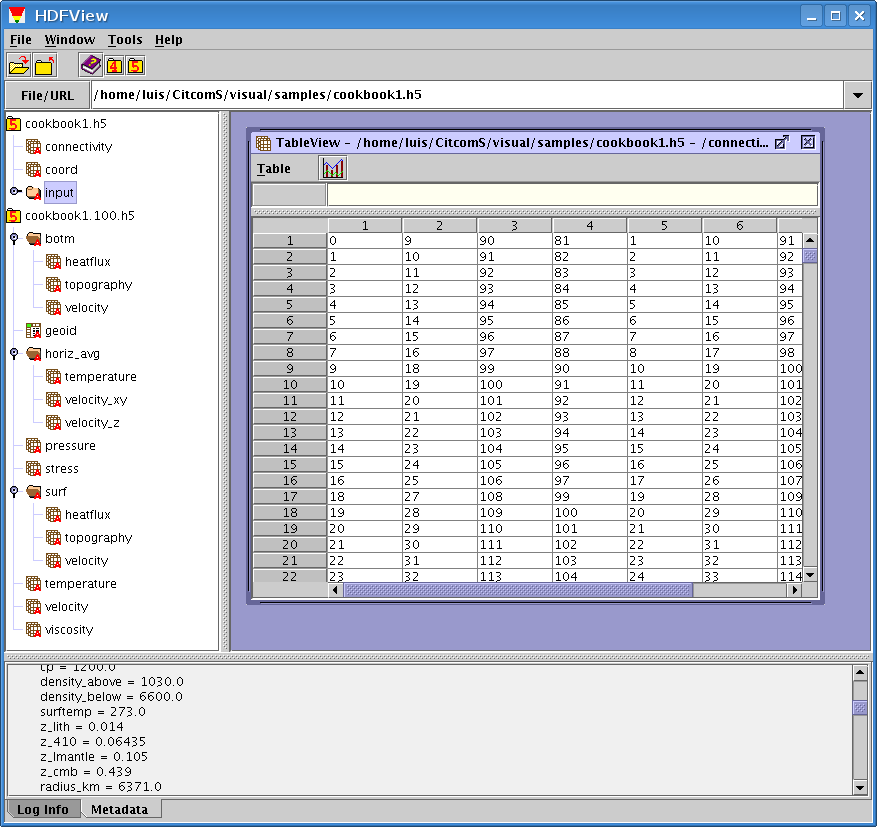
\includegraphics[scale=0.53]{graphics/hdfview.png}
\par\end{centering}

\caption{\label{fig:A-screenshot-of}A screenshot of HDFView. The left panel
shows the hierarchy of the groups and datasets. The right panel shows
a 2D slice of a dataset. The bottom panel shows the metadata associated
with the selected group or dataset.}
\end{figure}

\par\end{center}


\chapter{\label{cha:Postprocessing-and-Graphics}Postprocessing and Graphics}


\section{Introduction}

Once you have run CitcomS, you would have a series of output files
(potentially spread throughout the file systems of your Beowulf cluster
or in a set of directories on your parallel file system). You now
have to retrieve and combine the data for the time step (or age) of
interest. To visualize your results, it is recommended that you use
the open-source Open Visualization Data Explorer, better known as
OpenDX. The software is available from the OpenDX website \url{www.opendx.org}.
If you are using Linux, OpenDX is usually available as package \texttt{dx}
or \texttt{opendx} in your distribution. If you are using Mac OS X,
OpenDX is available via Fink \url{fink.sourceforge.net}. We provide
experimental scripts for a 3D visualization program called MayaVi2;
see Section \vref{sec:Using-MayaVi-for}. Scripts using GMT commands
to plot 2D cross sections of temperature field are also provided;
see Section \vref{sec:Using-GMT-Commands}. 


\section{Postprocessing on a Beowulf Cluster}

Generally, the results from your CitcomS run will be distributed on
disks attached to individual nodes of your Beowulf cluster. The output
files are written in each node under the directory that you specified
as the \texttt{datadir} property in the input file. To examine those
files, log in to a node and change directories to the one you specified
with a prefix. For example, if you set \texttt{datadir=/scratch/}\texttt{\emph{username}}
and \texttt{datafile=test-case} in your input file, then your output
files will be written to \texttt{/scratch/}\texttt{\emph{username}}
and will have the prefix \texttt{test-case}. 

If you select HDF5 for the output format, the output files will have
a \texttt{.h5} suffix. You won't need to postprocess the \texttt{.h5}
files; you can visualize the results using OpenDX. See Section \vref{sec:Using-OpenDX-for-HDF5}
for more details.

If you select compressed ASCII \texttt{(ascii-gz)} for the output
format, there is no post-processing script for it. You need to decompress
and rename the output files before you can use the post-processing
script described below.

If you select ASCII for the output format, you will have many output
files. An example of a filename for the velocity output is \texttt{test-case.velo.2.10}
where \texttt{test-case} is the model prefix, \texttt{velo} means
that this is a velocity data file, \texttt{2} corresponds to the processor
number (i.e., it is output by the 2nd processor), and \texttt{10}
corresponds to the time step. 

If your run used the time-dependent velocity boundary conditions (\texttt{solver.param.file\_vbcs=on}),
the log file will also have a \texttt{current age} line that lists
the time-step numbers and their corresponding times. To choose an
age to export for postprocessing, you have to determine which time
step corresponds to the age that interests you by looking at the log
file.

When you execute a CitcomS run, your input parameters will be saved
in a file \texttt{pidxxxxx.cfg} where \texttt{xxxxx} is usually a
five-digit number for the process ID. This pidfile contains most of
the input parameters, which can be useful for archiving and postprocessing. 

The ASCII output files of CitcomS need to be postprocessed before
you can perform the visualization. The script \texttt{autocombine.py}
can postprocess (retrieve and combine) CitcomS output; it will retrieve
CitcomS data to the current directory and combine the output into
a few files.

Using \texttt{autocombine.py}, retrieve and combine data of time-step
10: 
\begin{lyxcode}
\$~autocombine.py~mpirun.nodes~pid12345.cfg~10~
\end{lyxcode}
This reads the MPI machinefile (\texttt{mpirun.nodes}) and the CitcomS
pidfile (\texttt{pid12345.cfg}), then calls other scripts to do the
actual job. The general usage for \texttt{autocombine.py} is: 
\begin{lyxcode}
\$~autocombine.py~{[}machinefile{]}~{[}pidfile{]}~\textbackslash{}~\\
{[}step1{]}~{[}step2~or~more~...{]}~
\end{lyxcode}
If your Beowulf cluster uses \texttt{ssh} (rather than \texttt{rsh})
to access the computation nodes, you must manually edit \texttt{visual/batchpaste.sh}
and replace `rsh' with `ssh' in the script. 

Once \texttt{autocombine.py} has run, you will have 2 files (or 24
files for the full spherical version of CitcomS) formatted as follows: 
\begin{lyxcode}
test-case.cap00.10~\\
test-case.cap00.10.general
\end{lyxcode}
The former file is the data file containing simulation results and
is referred to as the ``capfile''; its format can be found in Appendix
\ref{cha:Appendix-C:-CitComS,}. The latter file is the OpenDX header
for the data.

If you have enabled some \texttt{optional\_output}, and the optional
fields are node-based (e.g, \texttt{comp\_nd}, \texttt{stress}, or
\texttt{pressure}), these fields will be combined in separated files,
with filenames:
\begin{lyxcode}
test-case.opt00.10~\\
test-case.opt00.10.general
\end{lyxcode}
The former file is the data file containing optional fields and is
referred to as the ``optfile.'' Its format is column-based ASCII data.
The latter file is the OpenDX header for the data. The header file
contains information on the ordering of the optional fields.


\section{Postprocessing in a Non-Cluster Environment}

If you run CitcomS in a non-cluster environment or all of your data
can be accessed from the local machine, you can still use \texttt{autocombine.py}
to combine the data. In this case, the \texttt{machinefile} is not
needed and can be replaced by \texttt{localhost}, such as: 
\begin{lyxcode}
\$~autocombine.py~localhost~{[}pidfile{]}~\textbackslash{}~\\
{[}step1{]}~{[}step2~or~more~...{]}~
\end{lyxcode}

\section{Using OpenDX for Regional Sphere Visualization}

OpenDX modules designed for CitcomS can be found in the source directory
called \texttt{visual}. The optional \texttt{make install} command
installs the OpenDX modules under \texttt{PREFIX/share/CitcomS/visual}
(where \texttt{PREFIX} defaults to \texttt{/usr/local}).

In this example, you will use \texttt{visRegional.net} to visualize
the results of regional CitcomS. 
\begin{enumerate}
\item Launch OpenDX by typing: 

\begin{lyxcode}
\$~dx~
\end{lyxcode}

You will see an OpenDX \textsf{Data Explorer} window. 

\item Click \textsf{Edit Visual Programs} and select \texttt{visRegional.net}
from the file selector. 
\item You will see a \textsf{Visual Program Editor} window. 
\item Select the \textsf{import} tab in the \textsf{Visual Program Editor}'s
main window and double-click on the \textsf{FileSelector} block, which
will open a \textsf{Control Panel} window. 
\item In the \textsf{CitcomSImport filename} input box, select the header
file of your postprocessed data, e.g.,

\begin{lyxcode}
samples/regtest.cap00.100.general
\end{lyxcode}
\item In the pull-down menu, select \textsf{Execute $\triangleright$ Execute
on Change}. 
\item A new window will appear with the image of the model. 
\item If you want to zoom, rotate, change projection, and otherwise manipulate
the view of the model, experiment with the menu \textsf{Options $\triangleright$
View Control}.
\end{enumerate}
\noindent \begin{center}
\begin{figure}[H]
\begin{centering}
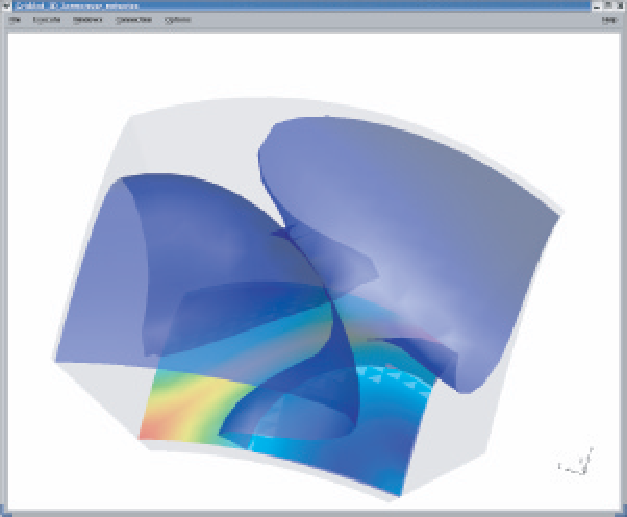
\includegraphics{graphics/c_fig5.pdf}
\par\end{centering}

\caption{Regional Model Visualized with OpenDX. A snapshot of an upwelling
(blue isosurface) with a slice of the temperature field (bisecting
plane).}
\end{figure}

\par\end{center}

Additional options in the control panel window for the regional model
include:
\begin{itemize}
\item \textsf{\textbf{CitcomSImport reduced}} can increase or reduce the
resolution of the velocity vectors and grids. Reducing resolution
is often necessary for visualizing large dataset interactively. Note
that the resolution of other fields (e.g., temperature and viscosity)
is not reduced.
\item \textsf{\textbf{Core radius}} is the size of the orange sphere which
represents the core-mantle boundary.
\item \textsf{\textbf{Isosurface value}} is the temperature isosurfaces.
You can change the values of the isosurfaces, including adding additional
isosurfaces or deleting existing ones. 
\item \textsf{\textbf{Slab cut dimension}} is the direction of the slab
(an OpenDX term for cross-section). 
\item \textsf{\textbf{Slab cut position}} is the position of the slab.  
\end{itemize}
You can change any of the parameters, visualization, or set-up by
going back to the main window and clicking on each tab. If you click
on each block, you will be able to change the settings for that function. 


\section{Using OpenDX for Full Sphere Visualization}
\begin{enumerate}
\item After launching OpenDX, you will see an OpenDX \textsf{Data Explorer}
window. 
\item Click \textsf{Edit Visual Programs} and select \texttt{visFull.net}
from the file selector. 
\item You will see a \textsf{Visual Program Editor} window. 
\item Select the \textsf{import} tab in the \textsf{Visual Program Editor}'s
main window and double-click on the \textsf{FileSelector} block, which
will open a \textsf{Control Panel} window. 
\item In the \textsf{Format String of CitcomSFullImport} input box, select
one of the 12 header files of your postprocessed data, e.g.,

\begin{lyxcode}
samples/fulltest.cap00.100.general
\end{lyxcode}
\item The results of a full spherical CitcomS consist of 12 cap files. In
order to import the 12 cap files at the same time, edit the filename
with the cap number replaced by printf-styled format string \texttt{\%02d},
e.g.,

\begin{lyxcode}
samples/fulltest.cap\%02d.100.general
\end{lyxcode}
\item In the pull-down menu, select \textsf{Execute $\triangleright$ Execute
on Change}. 
\item A new window will appear with the image of the model. 
\item If you want to zoom, rotate, change projection, and otherwise manipulate
the view of the model, experiment with the menu \textsf{Options $\triangleright$
View Control}.
\end{enumerate}
Additional options in the control panel window for the spherical model
include:
\begin{itemize}
\item \textsf{\textbf{CitcomSFullImport reduced}} can increase or reduce
the resolution of the velocity vectors and grids. Reducing resolution
is often necessary for visualizing large dataset interactively. Note
that the resolution of other fields (e.g., temperature and viscosity)
is not reduced.
\item \textsf{\textbf{Core radius}} is the size of the orange sphere which
represents the core-mantle boundary.
\item \textsf{\textbf{Isosurface value}} is the temperature isosurfaces.
You can change the values of the isosurfaces, including adding additional
isosurfaces or deleting existing ones. 
\item \textsf{\textbf{Latitude of normal axis}} and \textsf{\textbf{Longitude
of normal axis}} are the directions of the normal axis to the cross-section
plane.
\end{itemize}

\section{\label{sec:Using-OpenDX-for-HDF5}Using OpenDX for HDF5 Visualization}

If you use the HDF5 output format (\texttt{solver.output.output\_format=hdf5}),
you can directly visualize the data without postprocessing. First,
you need to install and set up the OpenDXutils package (see Section
\vref{sub:OpenDXutils}). Then, open either \texttt{visRegional.net}
or \texttt{visFull.net} in OpenDX. 
\begin{enumerate}
\item In the pull-down menu, select \textsf{File $\triangleright$ Load Macro,}
and select the file \textsf{CitcomSImportHDF5.net} to load it. 
\item In the \textsf{Tools} panel of the main window, select the \textsf{CitcomSImportHDF5}
module in the \textsf{Macros} category (highlighted in Figure \ref{fig:Import-CitComS.py-HDF5}). 
\item Place the module in the work space and rewire the network as shown
in Figure \ref{fig:Import-CitComS.py-HDF5}. 
\begin{figure}[t]
\noindent \begin{centering}
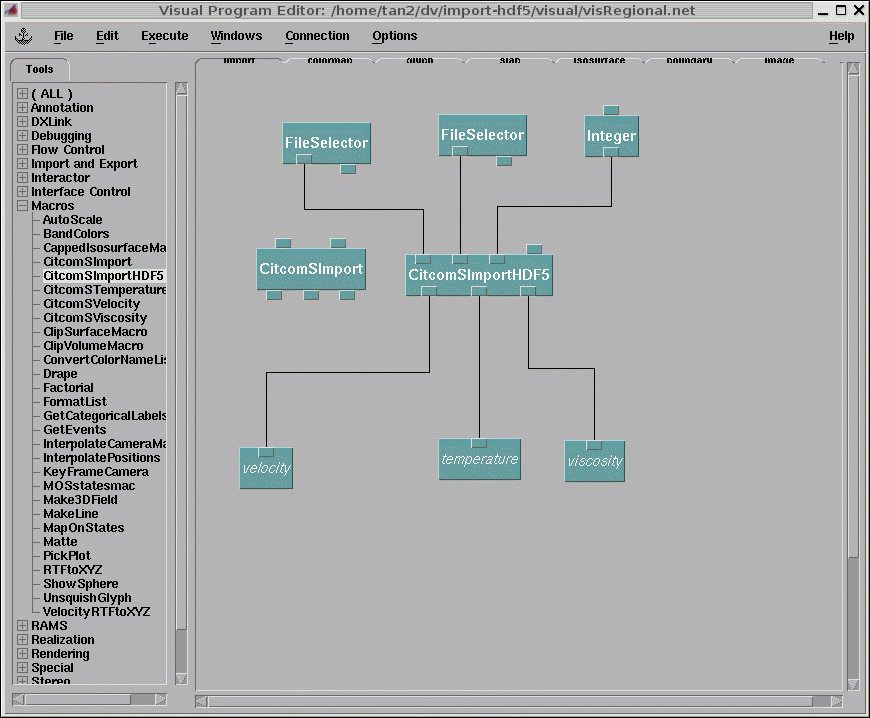
\includegraphics[width=0.75\paperwidth,keepaspectratio]{graphics/CitcomSImportHDF5.png}
\par\end{centering}

\caption{\label{fig:Import-CitComS.py-HDF5} How to import CitcomS HDF5 data.
The \textsf{CitcomSImportHDF5} module is highlighted in the Tools
panel.}
\end{figure}

\item There are four input tabs in the \textsf{CitcomSImportHDF5} module. 

\begin{enumerate}
\item The first tab (connected to the left \textsf{FileSelector} module)
specifies the HDF5 file containing time-independent information (e.g.,
\texttt{samples/cookbook1.h5}). 
\item The second tab (connected to the right \textsf{FileSelector} module)
specifies the HDF5 file containing time-dependent information (e.g.,
\textsf{samples}\texttt{/cookbook1.100.h5}).
\item The third tab (connected to the \textsf{Integer} module) specifies
the resolution reduction factor. 
\item The fourth tab (unconnected, default to 0) specifies which cap(s)
to import. 

\begin{enumerate}
\item To visualize a regional model, leave this tab unchanged. 
\item To visualize a full spherical model, double-click this module and
change the value of this tab to \texttt{\{0,1,2,3,4,5,6,7,8,9,10,11\}}. 
\item You can also specify a subset of caps to visualize.
\end{enumerate}
\end{enumerate}
\item After the data are imported, the visualization can be manipulated
as described in previous sections.
\end{enumerate}

\section{\label{sec:Using-MayaVi-for}Using MayaVi for Visualization}

This distribution also comes with scripts for visualizing CitcomS
using MayaVi2. MayaVi2 is the successor of MayaVi for 2D/3D scientific
data visualization. It is an interactive program allowing elaborate
plots of scientific data. MayaVi2 relies on the Visualization Toolkit
(VTK) and allows easy scripting in Python. To install MayaVi2, you
should follow the instructions on the MayaVi2 website \url{https://svn.enthought.com/enthought/wiki/GrabbingAndBuilding}
and on the SciPy website \url{www.scipy.org/Cookbook/MayaVi/Installation}.
Besides MayaVi2, before using the script you will need to install
PyTables (see Section \vref{sub:PyTables}) and PyVTK; see PyVTK website
\url{cens.ioc.ee/projects/pyvtk} for instructions.

The script acts as an extension module of MayaVi2. The installation
of the script is still preliminary. You will need to include \texttt{PREFIX/share/CitcomS/visual/Mayavi2/citcoms\_plugins/}
in your \texttt{PYTHONPATH} environment variable. You also need to
create a directory called \texttt{\textasciitilde{}/.mayavi2} and
copy into it the following: 
\begin{lyxcode}
PREFIX/share/CitcomS/visual/Mayavi2/mayavi\_custom\_ui.py
\end{lyxcode}
To run the script, type this command:
\begin{lyxcode}
\$~mayavi2\_citcoms\_display.py~\textit{file.step.h5}
\end{lyxcode}
This will launch MayaVi2 and load the data from \texttt{file.step.h5}.
An example of using this script is found in Figure \ref{fig:Example-MayaVi2-visualization}.
You may adjust your visualization pipeline by adding any appropriate
VTK filters and modules. For more details about this process, refer
to \textit{The Visualization Toolkit User's Guide} (ISBN 1-930934-13-0)
or see the VTK website \url{www.vtk.org}.

\noindent \begin{center}
\begin{figure}[H]
\noindent \begin{centering}
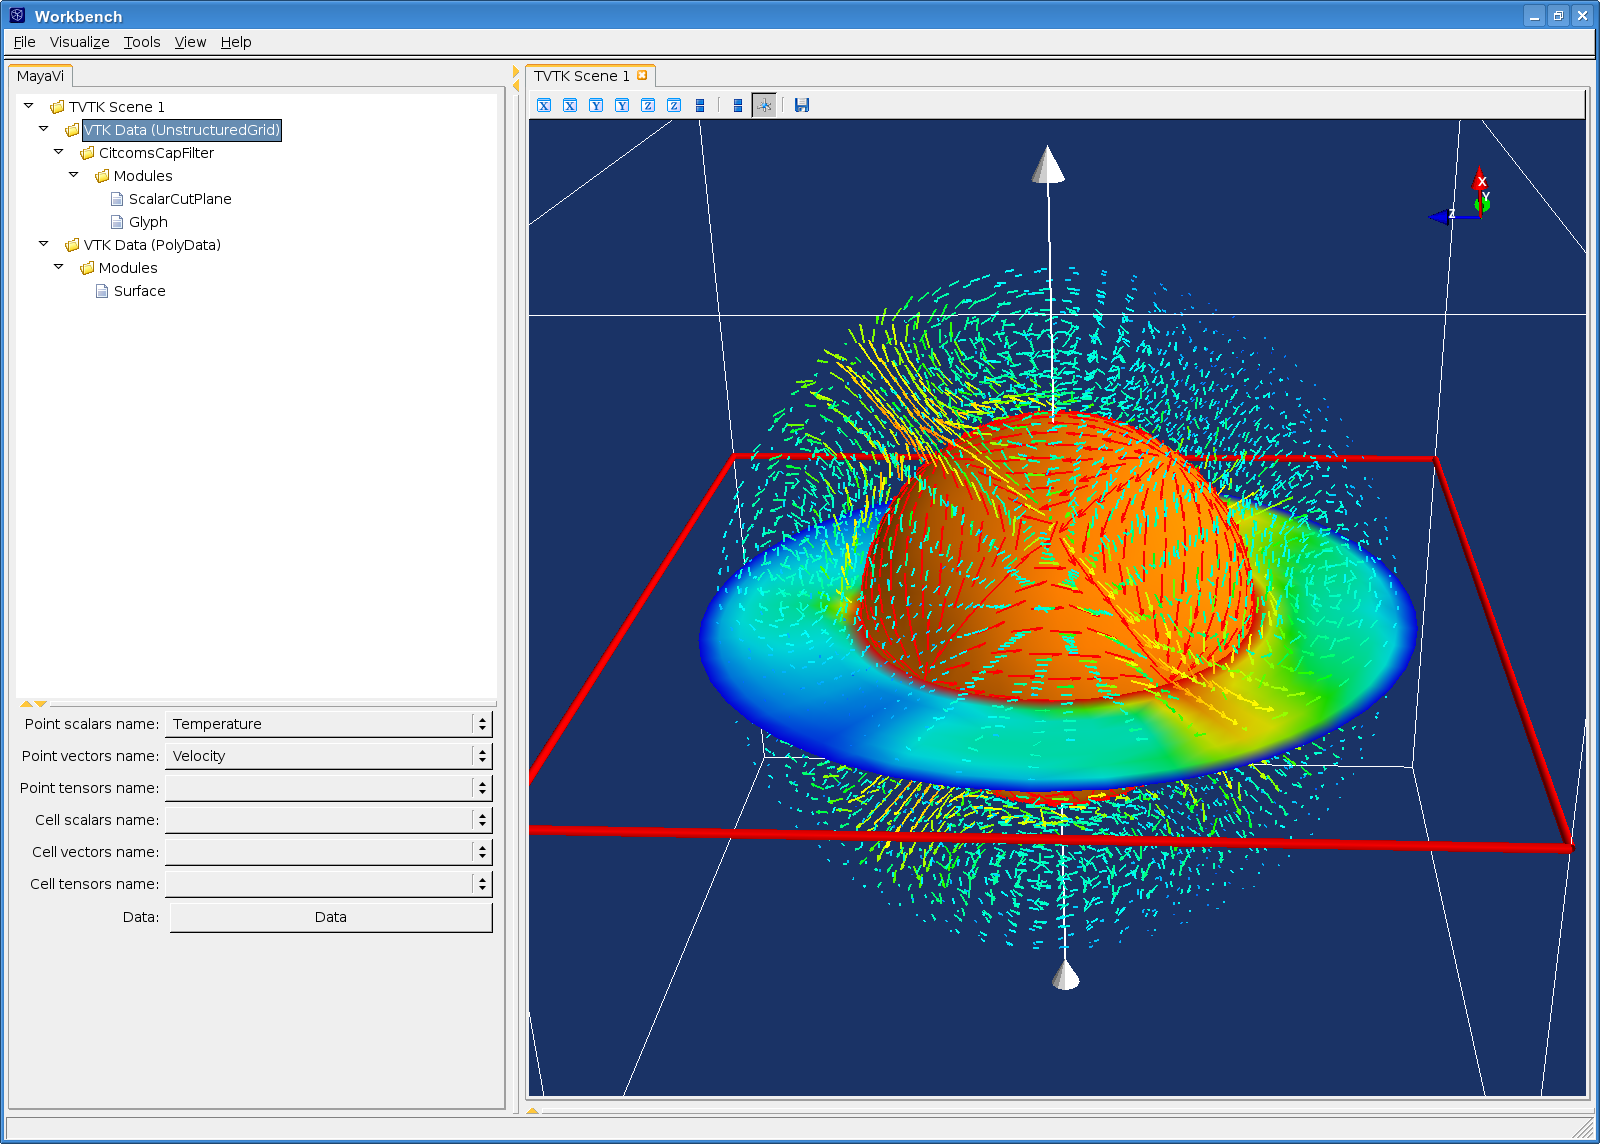
\includegraphics[scale=0.29]{graphics/mayavi2.png}
\par\end{centering}

\caption{\label{fig:Example-MayaVi2-visualization}Example MayaVi2 visualization
of \texttt{\small{cookbook1.100.h5}}. Here we display the velocity
field as vectors, as well a slice of the temperature field. Note the
visualization pipeline in the tree view on the left panel.}
\end{figure}

\par\end{center}


\section{\label{sec:Using-GMT-Commands}Using GMT Commands for Visualization}

The Generic Mapping Tools (GMT) is a collection of command-line tools
for manipulating geographic and Cartesian data that produces PostScript
(PS) or Encapsulated PostScript File (EPS) illustrations. GMT is widely
used in the geophysics community. Two scripts \texttt{plot\_layer.py}
and \texttt{plot\_annulus.py}, which can plot the temperature field
in horizontal and radial cross sections, respectively, are provided.
These scripts use GMT commands to generate EPS images. GMT is very
customizable. Users might wish to customize the scripts for their
need.

The usage of \texttt{plot\_layer.py} is:
\begin{lyxcode}
\$~plot\_layer.py~modelname~caps~step~layer
\end{lyxcode}
The script will look for the capfile(s) \texttt{modelname.cap00.step},
if \texttt{caps} is 1, or \texttt{modelname.cap00.step}, \texttt{modelname.cap01.step},
... through \texttt{modelname.cap11.step}, if \texttt{caps} is 12.
A slice of the capfile at the specified radial layer is then plotted
in Mercator projection, if \texttt{caps} is 1, or in Hammer-Aitoff
projection, if \texttt{caps} is 12.

\begin{figure}[H]
\noindent \begin{centering}
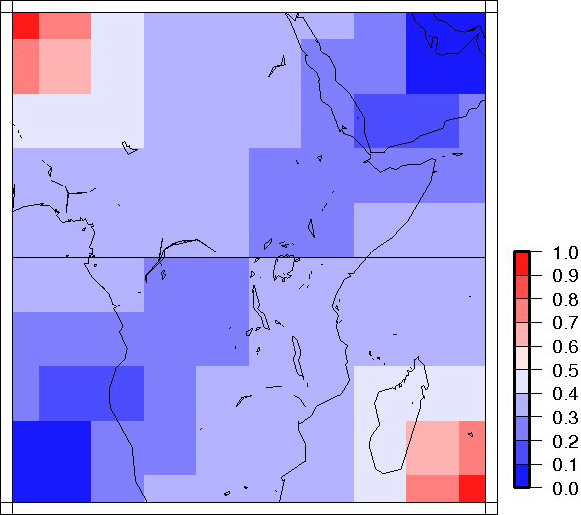
\includegraphics[scale=0.75]{graphics/regtest.jpg}
\par\end{centering}

\caption{Temperature field generated by \texttt{plot\_layer.py}. This image
is the mid-layer (layer 5) of the sample data \texttt{visual/samples/regtest.cap00.100}.
The resolution of the image is poor because the data has only 9$\times$9$\times$9
nodes.}
\end{figure}


The usage of \texttt{plot\_annulus.py} is:
\begin{lyxcode}
\$~plot\_annulus.py~modelname~step
\end{lyxcode}
The script will ask you a few questions on how to specify the great
circle path. There are three options: (1) a starting point and an
azimuth, (2) a starting point and another point on the great circle,
and (3) a starting point and a rotation pole. The great circle path
is used to construct the radial cross section.

\begin{figure}[H]
\noindent \begin{centering}
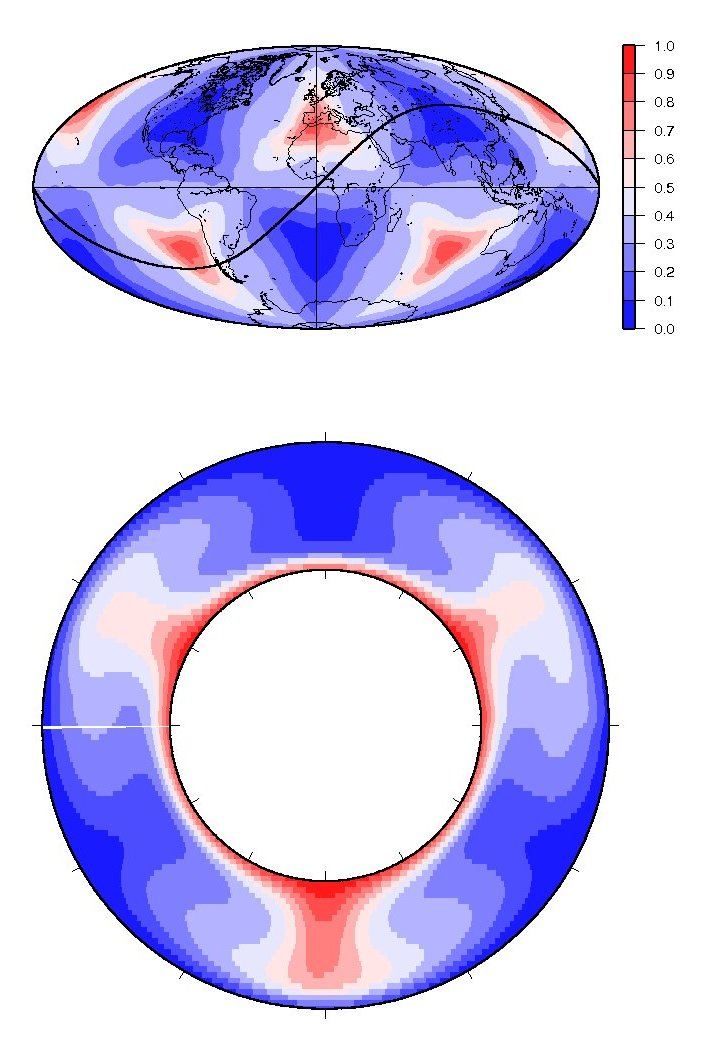
\includegraphics[scale=0.9]{graphics/fulltest.jpg}
\par\end{centering}

\caption{Temperature fields generated by \texttt{plot\_annulus.py}. The top
panel is the horizontal cross section at the mid layer in Hammer-Aitoff
projection. The thick line marks the surface track of the radial cross
section. The bottom panel is the radial cross section. The cross section
starts at $0^{\circ}$ latitude and $0^{\circ}$ longitude and has
an azimuth of ${45}^{\circ}$. The image is from the sample data \texttt{visual/samples/fulltest.cap{*}.100}.
There is always a gap on the left (starting point) of the cross section.
Users familiar with GMT are welcome to contribute a fix to the script.}
\end{figure}



\chapter{Cookbooks\label{cha:Cookbooks}}


\section{Introduction}

These cookbook examples are meant to serve as a guide to some of the
types of problems CitcomS can solve. Each of these cookbook problems
will only run with CitcomS if Pyre is enabled. Cookbook examples range
from regional to full spherical shell problems that address traditional
mantle convection problems. These cookbook examples are distributed
with the package under the \texttt{examples} directory. However, you
might need to edit these example scripts slightly to launch the job
on your cluster (see Section \vref{sec:Multiprocessor-Example} for
more information).

Cookbooks 1 to 4 introduce the basic parameters and are suitable for
all users. Cookbook 5 introduces time-dependent velocity boundary
conditions, reading in initial temperature field from files and tuning
of the advection solver. Cookbook 6 introduces the pseudo-free-surface
formulation for studying short wavelength dynamics topography. Cookbook
7 introduces thermo-chemical convection problem and tuning of the
Conjugate Gradient velocity solver. Cookbook 8 introduces compressible
convection problem, checkpointing/restarting, geoid and tuning of
the Multigrid and Uzawa velocity solver. Cookbook 9 introduces embedding
one CitcomS domain within another CitcomS domain, and further tuning
of the advection solver. Cookbook 10 introduces how to convert the
convection field to seismic velocities and how to generate synthetic
seismograms using SPECFEM3D\_GLOBE at the CIG Seismology Web Portal.\newpage{}


\section{\label{sec:Cookbook-1:-Global}Cookbook 1: Global Model}


\subsection{Problem}

This example solves for thermal convection within a full spherical
shell domain. The full spherical version of CitcomS is designed to
run on a cluster that decomposes the spherical shell into 12 equal
``caps'' and then distributes the calculation for caps onto separate
processors. To run CitcomS with the full solver parameter set, it
is recommended that you have a minimum of 12 processors available
on your cluster. 

\begin{figure}[h]
\begin{centering}
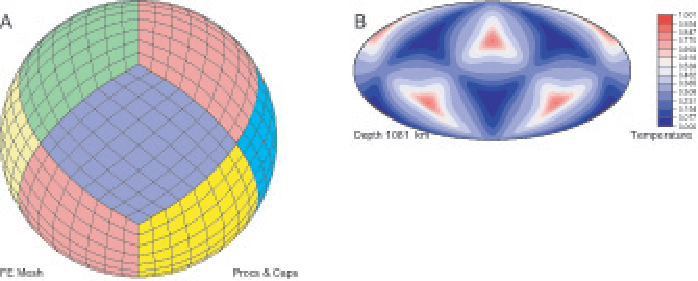
\includegraphics{graphics/cookbook1.pdf}
\par\end{centering}

\caption{Global Model ``Caps.'' Left (A): Three-dimensional perspective image
showing seven of the 12 spherical caps used in a full CitcomS run.
Right (B): The temperature field at 1081 km depth from a Cookbook
1 run.}
\end{figure}



\subsection{Solution}

You will use \texttt{cookbook1.cfg}. The first set of parameters specifies
that you are going to use the full spherical version of the solver.
The default is to use the regional spherical version, so this must
be set.
\begin{lyxcode}
solver~=~full
\end{lyxcode}
The second set of parameters specifies the number of time steps (100),
how often full outputs of the computation are created (25), and the
prefix of output filenames (cookbook1).
\begin{lyxcode}
steps~=~100~\\
monitoringFrequency~=~25~\\
datafile~=~cookbook1
\end{lyxcode}
The \texttt{solver.ic} facility controls the temperature field for
the initial conditions. The last set of parameters includes the number
of perturbations to the initial temperature (1), the number of nodal
lines of the perturbation in the longitudinal direction, e.g., the
spherical harmonic order (3), the number of nodal lines in the latitudinal
direction, e.g., the spherical harmonic degree (2), which layer the
perturbation is on (5), and the amplitude of the perturbation (0.05).
Note that although the number of perturbations is assigned here as
\texttt{num\_perturbations=1}, that is actually the default value.
\begin{lyxcode}
num\_perturbations~=~1~\\
perturbl~=~3~\\
perturbm~=~2~\\
perturblayer~=~5~\\
perturbmag~=~0.05
\end{lyxcode}
This example is executed by typing 
\begin{lyxcode}
\$~citcoms~cookbook1.cfg
\end{lyxcode}

\subsubsection{Example: Global Model, \texttt{cookbook1.cfg}}
\begin{lyxcode}
{[}CitcomS{]}~\\
solver~=~full~\\
steps~=~100~~~~~~~~~~~~~~~~~;~number~of~time~steps~\\
~\\
{[}CitcomS.controller{]}~\\
monitoringFrequency~=~25~~~~;~how~often~outputs~are~created~\\
~\\
{[}CitcomS.solver{]}~\\
datafile~=~cookbook1~~~~~~~~;~prefix~of~output~filenames~\\
~\\
{[}CitcomS.solver.ic{]}~\\
num\_perturbations~=~1~\\
perturbl~=~3~\\
perturbm~=~2~\\
perturblayer~=~5~\\
perturbmag~=~0.05~
\end{lyxcode}
Once you have run the model, you can visualize the results using OpenDX,
described in the previous chapter. When you invoke ``Edit Visual Program,''
select \texttt{visFull.net}. 

\begin{figure}[H]
\begin{centering}
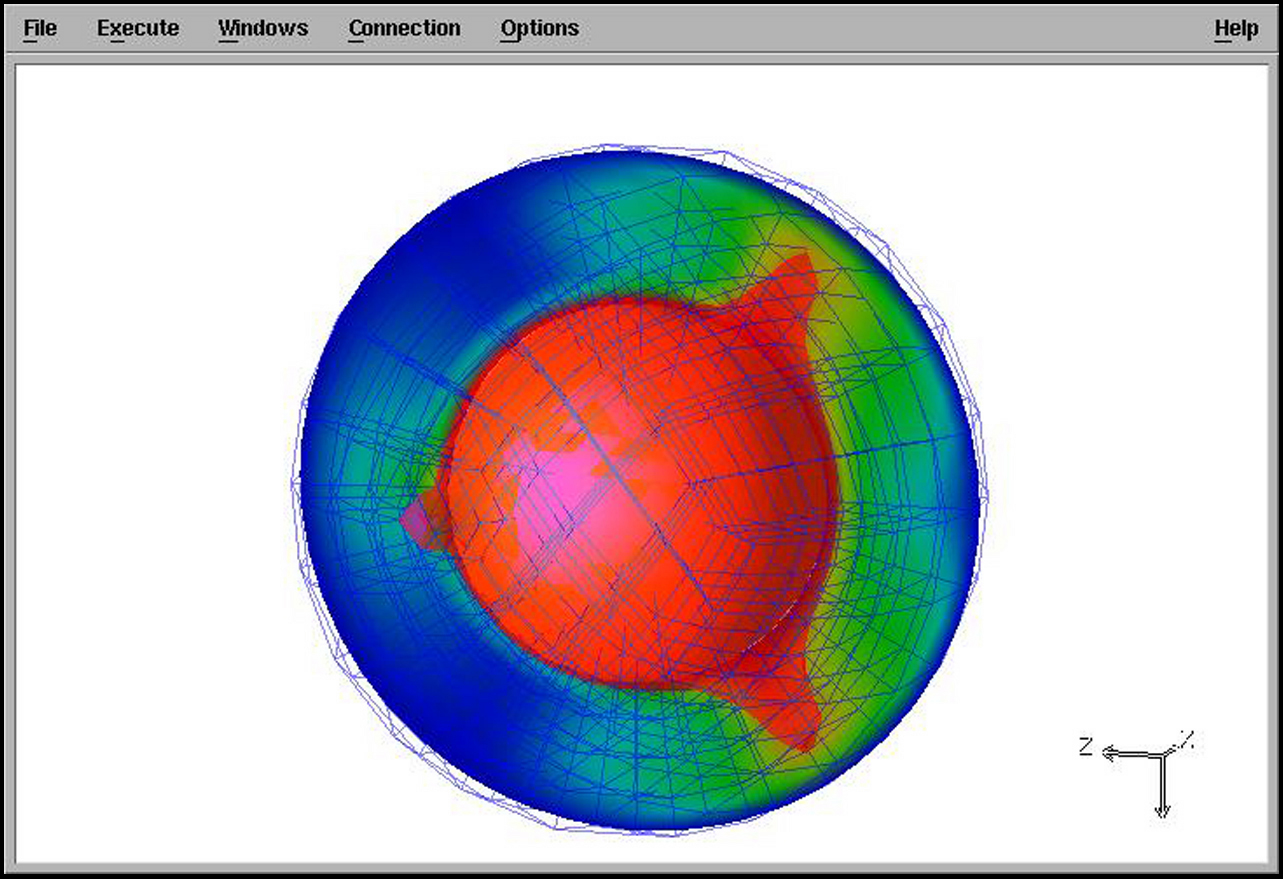
\includegraphics[scale=0.8]{graphics/cookbook1.jpg}
\par\end{centering}

\caption{Cookbook 1: Global Model. This image, created by OpenDX, depicts a
slice through a spherical model of convection, with warmer colors
indicating upwelling and the cooler colors showing downwelling.}
\end{figure}



\subsection{Discussion}

You have generated a simple example of the full CitcomS model, with
minimal parameter alterations. With a default Rayleigh number of $10^{5}$
and perturbation on the initial temperature field which has a degree-3
and an order-2 pattern, after 100 time steps, the convection pattern
remains relatively steady.

As a side note, it is not required that 12 processors, with one spherical
cap per processor, be used. As an end-member possibility, for example,
12 different jobs could be run on a single computer (\texttt{n001}
in this example) by invoking:
\begin{lyxcode}
\$~citcoms~cookbook1.cfg~-{}-launcher.nodegen=\textquotedbl{}n\%03d\textquotedbl{}~\textbackslash{}~\\
-{}-launcher.nodelist={[}1,1,1,1,1,1,1,1,1,1,1,1{]}
\end{lyxcode}
This is not particularly efficient, but it does illustrate the flexibility
of both MPI and Pyre.

\newpage{}


\section{Cookbook 2: Domain Size and Velocity Boundary Conditions}


\subsection{Problem}

This example solves for thermal convection with velocity boundary
conditions imposed on the top surface within a given region of a sphere.
This requires using the regional version of CitcomS. 


\subsection{Solution}

You will use \texttt{cookbook2.cfg}. The parameters specify the number
of time steps (60), the prefix of the output filenames (\texttt{cookbook2}),
and how often outputs will be created (30).
\begin{lyxcode}
steps~=~60~\\
monitoringFrequency~=~30~\\
datafile~=~cookbook2
\end{lyxcode}
The \texttt{solver.mesher} facility has several properties involved
in the generation of the computational mesh. Continue to use the default
values for the physical portion of the domain in which you are interested.
However, try modifying the layout of the mesh as shown. The parameters
specify two processors per cap in the $x$- and $y$-direction, one
processor per cap in the $z$-direction (by default), 17 nodes per
cap in the $x$- and $y$-direction, 9 nodes in the $z$-direction,
and the minimum/maximum extents in the colatitudal, longitudal, and
radial (\texttt{theta}, \texttt{fi}, \texttt{radius}) directions.
The unit for \texttt{theta} and \texttt{fi} is radian.
\begin{lyxcode}
nprocx~=~~2~\\
nprocy~=~~2~\\
nodex~~=~17~\\
nodey~~=~17~\\
nodez~~=~~9~\\
~\\
theta\_min~=~0.7854~\\
theta\_max~=~1.5708~\\
fi\_min~=~0.0~\\
fi\_max~=~0.7854~\\
radius\_inner~=~0.55~\\
radius\_outer~=~1.0
\end{lyxcode}
The \texttt{solver.bc} facility allows you to impose a uniform velocity
across the top surface. You have a velocity which is purely in the
colatitude direction with a non-dimensional velocity of 100 (see Equation
\vref{eq:u dim} for how to dimensionalize it).
\begin{lyxcode}
topvbc~~~~=~~~1~\\
topvbxval~=~100~\\
topvbyval~=~~~0
\end{lyxcode}
In addition, the initial temperature field has a linear conductive
profile. The amplitude of initial temperature perturbation is set
to zero using the \texttt{solver.ic} facility. 
\begin{lyxcode}
num\_perturbations~=~1~\\
perturbmag~~~~~~~~=~0.0~
\end{lyxcode}

\subsubsection{Example: Velocity Boundary Conditions, \texttt{cookbook2.cfg}}
\begin{lyxcode}
{[}CitcomS{]}~\\
steps~=~60~~~~~~~~~~~~~~~~~~;~number~of~time~steps~\\
~\\
{[}CitcomS.controller{]}~\\
monitoringFrequency~=~30~~~~;~how~often~outputs~are~created~\\
~\\
{[}CitcomS.solver{]}~\\
datafile~=~cookbook2~~~~~~~~;~prefix~of~output~filenames~\\
~\\
\#~Modify~the~layout~of~the~mesh.~\\
{[}CitcomS.solver.mesher{]}~\\
nprocx~=~~2~\\
nprocy~=~~2~\\
nodex~~=~17~\\
nodey~~=~17~\\
nodez~~=~~9~\\
~\\
theta\_min~=~0.7854~\\
theta\_max~=~1.5708~\\
fi\_min~=~0.0~\\
fi\_max~=~0.7854~\\
radius\_inner~=~0.55~\\
radius\_outer~=~1.0~\\
~\\
\#~Impose~a~uniform~velocity~across~the~top~surface.~\\
{[}CitcomS.solver.bc{]}~\\
topvbc~~~~=~~~1~\\
topvbxval~=~100~\\
topvbyval~=~~~0~\\
~\\
\#~In~addition,~set~the~initial~temperature~perturbation~to~zero.~\\
{[}CitcomS.solver.ic{]}~\\
num\_perturbations~=~1~\\
perturbmag~~~~~~~~=~0.0~
\end{lyxcode}

\subsection{Discussion}

Using OpenDX to visualize the results (Figure \ref{fig:Cookbook-2:-Velocity}),
this model allows you to create a plate-driven convection in which
there is a thermal upwelling on one wall, a thermal downwelling on
another, and uniform horizontal velocity across the top. The downwelling
is not exactly subduction because the sidewalls have reflecting boundary
conditions. This means that there is a symmetrical downwelling in
a vertical domain on the other side.

\begin{figure}[h]
\begin{centering}
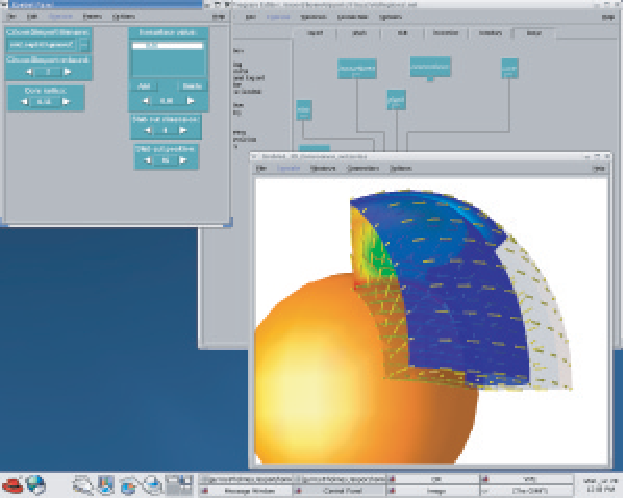
\includegraphics{graphics/cookbook2dot2.pdf}
\par\end{centering}

\caption{\label{fig:Cookbook-2:-Velocity}Cookbook 2: Velocity Boundary Conditions.
This model, visualized with OpenDX, highlights a region of the sphere
and the heated upwellings (warm colors), downwellings (cool colors),
and the velocities (yellow arrows).}
\end{figure}


\newpage{}


\section{Cookbook 3: Temperature-Dependent Viscosity}


\subsection{Problem}

A common problem in geophysics is the exploration of natural convection
in the presence of variable viscosity, including temperature-dependent
or stress-dependent viscosity.


\subsection{Solution}

You will use \texttt{cookbook3.cfg}. The parameters specify the number
of time steps (200), how often outputs will be created (25), the prefix
of the output filenames (\texttt{cookbook3}), and the Rayleigh number
($10^{6}$).
\begin{lyxcode}
steps~=~200~\\
monitoringFrequency~=~25~\\
datafile~=~cookbook3~\\
rayleigh~=~1e6
\end{lyxcode}
The \texttt{solver.visc} facility assigns the viscosities. The parameters
specify whether the viscosity should be updated at every time step
(\texttt{on}), the number of viscous layers (4), the viscosity of
each layer (1,1,1,1), whether the viscosity is temperature dependent
(\texttt{on}), the type of viscosity law to use (4), the activation
energy of each layer (0.2,0.2,0.2,0.2), the temperature offset of
each layer (0,0,0,0), the activation volume of each layer (0,0,0,0),
whether to apply the minimum cutoff (\texttt{on}), the value of the
minimum cutoff (1.0), whether to apply the maximum cutoff (\texttt{on}),
and the value of the maximum cutoff (100.0). 
\begin{lyxcode}
VISC\_UPDATE~=~on~\\
num\_mat~=~4~\\
visc0~=~1,1,1,1~\\
TDEPV~=~on~\\
rheol~=~4~\\
viscE~=~0.2,0.2,0.2,0.2~\\
viscT~=~0,0,0,0~\\
viscZ~=~0,0,0,0~\\
VMIN~=~on~\\
visc\_min~=~1.0~\\
VMAX~=~on~\\
visc\_max~=~100.0
\end{lyxcode}
The range of the layers are determined by the following parameters:
layer 1 extends from the top surface to a depth of \texttt{solver.const.z\_lith}
(default to 0.014, or 90 km dimensionally); layer 2 is below layer
1 and extends to a depth of \texttt{solver.const.z\_410} (default
to 0.06435, or 410 km dimensionally); layer 3 is below layer 2 and
extends to a depth of \texttt{solver.const.z\_lmantle} (default to
0.105, or 670 km dimensionally); layer 4 is below layer 3 and extends
to the bottom. These depth parameters also control the depth of various
phase transitions.

There are several viscosity laws coded in the program, which can be
selected by the \texttt{rheol} parameter. All available viscosity
laws can be found in Appendix \ref{sub:Viscosity-input}. For \texttt{rheol=4},
the temperature dependence of the viscosity of each layer is determined
by: 

\begin{equation}
visc=visc0\times exp\left(\frac{viscE+viscZ\times(1-r)}{T^{*}+viscT}-\frac{viscE+viscZ\times(1-r_{inner})}{1+viscT}\right)\label{eq:non-dim visc law}
\end{equation}
where $T^{*}=\min(\max(T,0),1)$. This equation is non-dimensionalized.
The last term on the right-hand side normalizes the viscosity such
that $visc=visc0$ when $T=1$ and $r=r_{inner}$. Comparing Equation
\ref{eq:non-dim visc law} with the dimensional Arrhenius activation
equation:
\begin{eqnarray}
\eta & = & \eta_{0}exp\left(\frac{E_{a}+PV_{a}}{RT}\right)=\eta_{0}exp\left(\frac{E_{a}+PV_{a}}{R\Delta T\left(T'+T_{0}'\right)}\right)\nonumber \\
 & = & \eta_{0}exp\left(\frac{E_{a}+\rho g\left(1-r\right)V_{a}}{R\Delta T\left(T'+T_{0}'\right)}\right)=\eta_{0}exp\left(\frac{E_{a}/R\Delta T+\left(1-r\right)\rho gV_{a}/R\Delta T}{T'+T_{0}'}\right)\label{eq:arrhenius}
\end{eqnarray}
where $E_{a}$ and $V_{a}$ are the activation energy and activation
volume, $P$ is the hydrostatic pressure, $R$ is the universal gas
constant, and other symbols are as defined in Section \ref{sec:Governing-Equations},
it is clear that
\begin{equation}
viscE=\frac{E_{a}}{R\Delta T}\label{eq:viscE}
\end{equation}
\begin{equation}
viscZ=\frac{\rho gV_{a}}{R\Delta T}\label{eq:viscZ}
\end{equation}
\begin{equation}
viscT=T_{0}\label{eq:viscT}
\end{equation}



\subsubsection{Example: Temperature-Dependent Viscosity, \texttt{cookbook3.cfg}}
\begin{lyxcode}
{[}CitcomS{]}~\\
steps~=~200~~~~~~~~~~~~~~~~~;~number~of~time~steps~\\
~\\
{[}CitcomS.controller{]}~\\
monitoringFrequency~=~25~~~~;~how~often~outputs~are~created~\\
~\\
{[}CitcomS.solver{]}~\\
datafile~=~cookbook3~~~~~~~~;~prefix~of~output~filenames~\\
rayleigh~=~1e6~~~~~~~~~~~~~~;~Rayleigh~number~\\
~\\
\#~Modify~the~layout~of~the~mesh.~\\
{[}CitcomS.solver.mesher{]}~\\
nprocx~=~~2~\\
nprocy~=~~2~\\
nodex~~=~17~\\
nodey~~=~17~\\
nodez~~=~~9~\\
~\\
\#~Assign~the~viscosities.~\\
{[}CitcomS.solver.visc{]}~\\
VISC\_UPDATE~=~on~\\
num\_mat~=~4~\\
visc0~=~1,1,1,1~\\
TDEPV~=~on~\\
rheol~=~4~\\
viscE~=~0.2,0.2,0.2,0.2~\\
viscT~=~0,0,0,0~\\
viscZ~=~0,0,0,0~\\
VMIN~=~on~\\
visc\_min~=~1.0~\\
VMAX~=~on~\\
visc\_max~=~100.0
\end{lyxcode}
\begin{figure}[H]
\begin{centering}
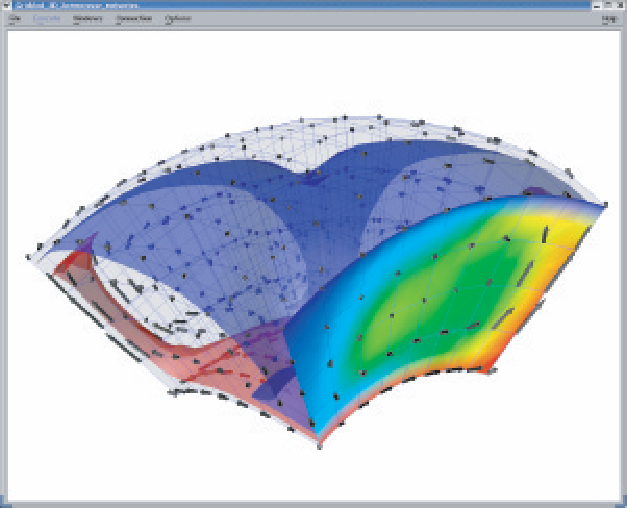
\includegraphics{graphics/cookbook3.pdf}
\par\end{centering}

\caption{Cookbook 3: Temperature-Dependent Viscosity. This model, visualized
with OpenDX, highlights a region that features both the heated upwelling
(warm colors) and the even distribution of the velocities (arrows).}
\end{figure}


\newpage{}


\section{Cookbook 4: Regionally Refined Meshes }


\subsection{Problem}

Frequently for convection problems, particularly those with variable
viscosity, there are features with strong gradients in temperature
or viscosity that can be better resolved with refined meshes. For
example, for the problem just studied in Cookbook 3, temperature-dependent
viscosity, a higher resolution is required for a narrow hot upwelling
while a lower resolution is sufficient for the wider cold downwelling. 


\subsection{Solution}

The parameter that controls whether a mesh is to be uniform or refined
is \texttt{solver.mesher.coor}. Set it to \texttt{1} \texttt{(solver.mesher.coor=1)}
in order to read the uneven mesh point coordinates from an input file
(specified by \texttt{coor\_file}). The format of the coordinate input
file is described in Appendix \vref{sec:Coordinate-files}.
\begin{lyxcode}
coor~=~1~\\
coor\_file~=~coor.dat
\end{lyxcode}
The computational domain is bounded in colatitude between radian 1
and 2, in latitude between radian 0 and 1, and in radius between 0.55
and 1, as determined by the content of \texttt{coor\_file}.


\subsubsection{Example: Regionally Refined Meshes, \texttt{cookbook4.cfg}}
\begin{lyxcode}
{[}CitcomS{]}~\\
steps~=~250~~~~~~~~~~~~~~~~~;~number~of~time~steps~\\
~\\
{[}CitcomS.controller{]}~\\
monitoringFrequency~=~10~~~~;~how~often~outputs~are~created~\\
~\\
{[}CitcomS.solver{]}~\\
rayleigh~=~1e6~~~~~~~~~~~~~~;~Rayleigh~number~\\
datafile~=~cookbook4~~~~~~~~;~prefix~of~output~filenames~\\
~\\
{[}CitcomS.solver.ic{]}~\\
num\_perturbations~=~1~\\
perturbmag~=~0.05~\\
perturblayer~=~10~\\
~\\
\#~Perturb~the~initial~temperature~gradient~in~the~longitudinal~\\
\#~direction.~\\
perturbl~=~1~\\
perturbm~=~0~\\
~\\
{[}CitcomS.solver.mesher{]}~\\
\#~Read~uneven~mesh~point~coordinates~from~'coor.dat'.~\\
coor~=~1~\\
coor\_file~=~coor.dat~\\
~\\
nprocx~=~2~\\
nprocy~=~1~\\
nprocz~=~1~\\
nodex~=~33~\\
nodey~=~17~\\
nodez~=~17~\\
~\\
{[}CitcomS.solver.visc{]}~\\
VISC\_UPDATE~=~on~\\
num\_mat~=~4~\\
visc0~=~1,1,1,1~\\
TDEPV~=~on~\\
rheol~=~4~\\
viscE~=~0.2,0.2,0.2,0.2~\\
viscT~=~0,0,0,0~\\
viscZ~=~0,0,0,0~\\
VMIN~=~on~\\
visc\_min~=~1.0~\\
VMAX~=~on~\\
visc\_max~=~100.0
\end{lyxcode}
\begin{figure}[H]
\begin{centering}
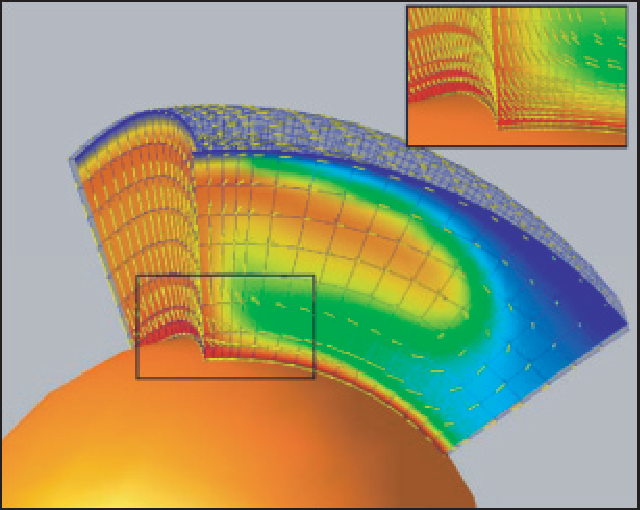
\includegraphics{graphics/cookbook4.pdf}
\par\end{centering}

\caption{Cookbook 4: Regionally Refined Mesher. This model shows the temperature
(upwelling -- warm colors, downwelling -- cool colors) and the uneven
distribution of the velocities (yellow arrows). Note the refined mesh
for the left and bottom regions of the model (inset).}
\end{figure}



\subsection{Discussion}

The resulting model is like a 2D model, but extends in the longitudinal
direction. To set up this type of model, the initial temperature gradient
was perturbed only in the longitudinal direction, by setting the parameters
\texttt{perturbl=1} and \texttt{perturbm=0}. The model results show
a thin thermal upwelling on one wall and a wide thermal downwelling
on the opposite wall. Also, at the bottom of the model a thin layer
of hot material can be shown. Note the higher resolution in the narrow
regions with hot material and the lower resolution for the wide thermal
downwelling region.

\newpage{}


\section{Cookbook 5: Subduction Models with Trench Rollback}


\subsection{Problem}

A common issue to address is the problem arising when the position
of the oceanic trench is not constant in time (trench rollback) for
a subduction zone. In addition, the trench rollback speed may vary
in time, which can be caused, for example, by a rotation pole jump. 


\subsection{Solution}

In order to introduce in a convection model a trench rollback you
have to prepare the velocity files. The following scenario is proposed
for this cookbook: there are two plates centered along the equator,
with two different Euler poles (see Figure \ref{fig:Cookbook-5:-Left}).
Initially, both plates have Euler poles situated far apart, so the
velocities are approximately constant (about 5 cm/yr for the left
plate and about 2 cm/yr for the right plate). After 30 Ma, a pole
jump occurred for the right slab only, so the Euler pole moved closer. 

Since we impose a top velocity boundary in our model, the following
parameters should be turned on: 
\begin{lyxcode}
{[}CitcomS.solver.bc{]}~\\
topvbc~=~1~\\
~\\
{[}CitcomS.solver.param{]}~\\
file\_vbcs~=~on
\end{lyxcode}
The following two lines specify the location of the velocity files
and the starting age for the model: 
\begin{lyxcode}
start\_age~=~55~\\
vel\_bound\_file~=~./velocity/bvel.dat~
\end{lyxcode}
Since the starting age is set to 55 Ma, there will be 57 velocity
files, one for each Ma (\texttt{vel.dat0, vel.dat1,} \texttt{...vel.dat55,
vel.dat56}). The format of the velocity file is described in Appendix
\vref{sec:Velocity-boundary-condition}. Note that the velocity file
uses a unit of cm/yr.

When \texttt{tic\_method=-1} is set, the initial temperature field
is read from setup files. The files have the same naming scheme and
format as the CitcomS velo output, as described in Appendix \vref{sub:Velocity-and-Temperature}.
The location and prefix of the file is specified in \texttt{datadir\_old}
and \texttt{datafile\_old}, and the time step of the velo file in
\texttt{solition\_cycles\_init}. In this example, a processor of MPI
rank \texttt{n} will read file \texttt{./ic/cookbook5.velo.n.0}
\begin{lyxcode}
{[}CitcomS.solver{]}~\\
datadir\_old~=~./ic~\\
datafile\_old~=~cookbook5~\\
~\\
{[}CitcomS.solver.ic{]}~\\
tic\_method~=~-1~~\\
solution\_cycles\_init~=~0
\end{lyxcode}
The descending slab will cause some numerical instability in the temperature
solver. To reduce the numerical instability, you will use a smaller
time-step size (0.75 of the maximum time-step size for a stable solution).
The change in maximum temperature will also be monitored. If the maximum
temperature increases too much (> 5\%) between time steps, the temperature
solver will rerun with half time-step size.
\begin{lyxcode}
{[}CitcomS.solver.tsolver{]}~\\
finetunedt~=~0.75~\\
monitor\_max\_T~=~on
\end{lyxcode}
\begin{figure}[H]
\begin{centering}
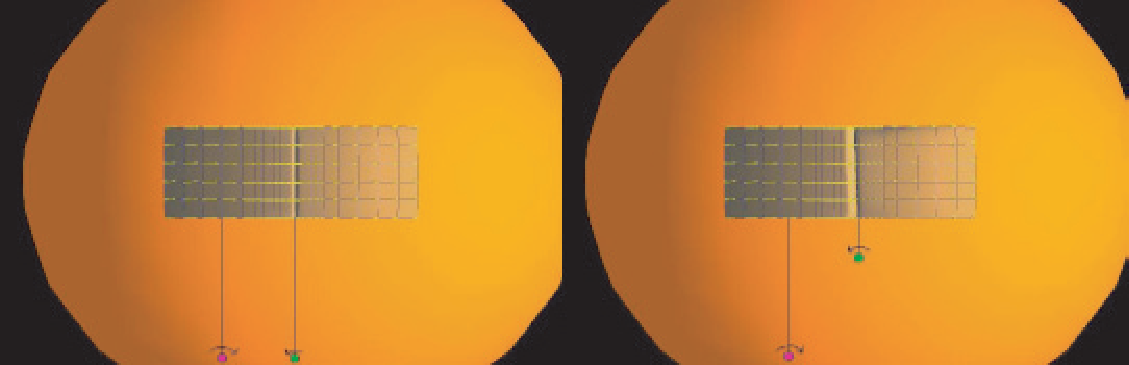
\includegraphics[scale=0.65]{graphics/cookbook5.pdf}
\par\end{centering}

\caption{\label{fig:Cookbook-5:-Left}Cookbook 5: Left (A): Initially, both
plates have Euler poles (magenta and green dots) situated far apart
from the plate, so the velocities are approximately constant (about
5 cm/yr for the left plate and about 2 cm/yr for the right plate).
Right (B): After 30 Ma a pole jump occurred for the right slab only,
so the Euler pole moved closer.}
\end{figure}



\subsubsection{Example: Subduction Models with Trench Rollback, \texttt{cookbook5.cfg}}
\begin{lyxcode}
{[}CitcomS{]}~\\
steps~=~1100~~~~~~~~~~~~~~~~;~number~of~time~steps~\\
~\\
{[}CitcomS.controller{]}~\\
monitoringFrequency~=~100~~~;~how~often~outputs~are~created~\\
~\\
{[}CitcomS.solver{]}~\\
datafile~=~cookbook5~\\
datadir\_old~=~./ic~\\
datafile\_old~=~cookbook5~\\
rayleigh~=~4.07e+08~\\
~\\
{[}CitcomS.solver.bc{]}~\\
topvbc~=~1~\\
~\\
{[}CitcomS.solver.param{]}~\\
file\_vbcs~=~on~\\
start\_age~=~55~\\
~\\
\#~Since~the~starting~age~is~set~to~55~Ma,~there~will~be~57~velocity~\\
\#~files,~one~for~each~Ma~(bvel.dat0,~bvel.dat1,~...~bvel.dat56).~\\
vel\_bound\_file~=~./velocity/bvel.dat~\\
~\\
{[}CitcomS.solver.ic{]}~\\
tic\_method~=~-1~\\
solution\_cycles\_init~=~0~\\
~\\
{[}CitcomS.solver.mesher{]}~\\
coor~=~1~\\
coor\_file~=~./coor.dat~\\
nprocx~=~1~\\
nprocy~=~2~\\
nprocz~=~1~\\
nodex~=~17~\\
nodey~=~65~\\
nodez~=~33~\\
~\\
{[}CitcomS.solver.tsolver{]}~\\
finetunedt~=~0.75~\\
monitor\_max\_T~=~on~\\
~\\
{[}CitcomS.solver.visc{]}~\\
num\_mat~=~4~\\
visc0~=~100,0.003,1,2~\\
TDEPV~=~on~\\
viscE~=~24,24,24,24~\\
viscT~=~0.182,0.182,0.182,0.182~\\
VMIN~=~on~\\
visc\_min~=~0.01~\\
VMAX~=~on~\\
visc\_max~=~100.0~
\end{lyxcode}
\begin{figure}[H]
\begin{centering}
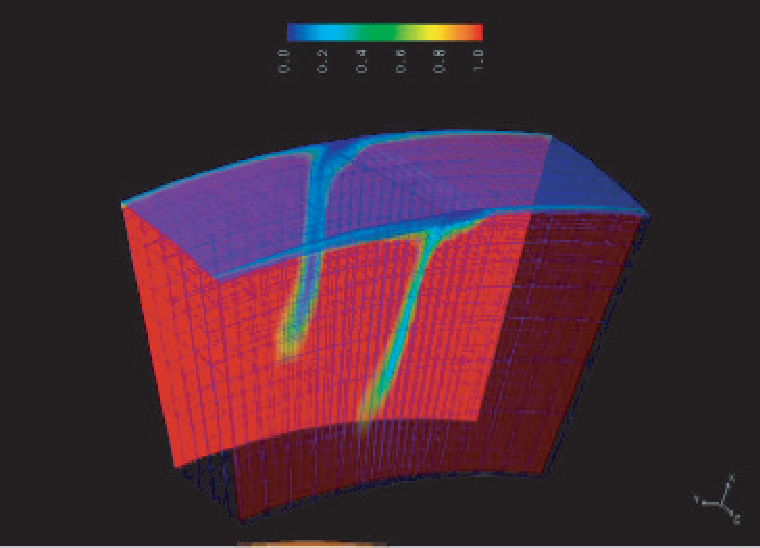
\includegraphics{graphics/cookbook5dot2.pdf}
\par\end{centering}

\caption{\label{fig:Cookbook-5:-the}Cookbook 5: The pole jump after 30 Ma
produced a flat slab on one side (fore side) and a steep slab on the
other side (back side). }
\end{figure}



\subsection{Discussion}

The results for this problem are presented in Figure \ref{fig:Cookbook-5:-the}.
Since the two Euler poles are kept fixed for the first 30 Ma, the
shape of the subducting slab will be the same along the trench. At
25 Ma, the Euler pole for the right plate jumps toward the plate.
Therefore, the velocity along the trench varies from about 1 cm/yr
to about 2.5 cm/yr. This will produce in time a flat slab at one side
of the model, and a steep slab at the other side.

\newpage{}


\section{Cookbook 6: Pseudo-Free-Surface Formulation}


\subsection{Problem}

Free-slip boundary conditions are typically applied on the top surface
of mantle convection models, and the dynamic topography is obtained
by assuming that the normal stress on the top surface is instantaneously
compensated by the deformed surface. This type of boundary condition
works well for long-wavelength topography, but a free-surface formulation
becomes necessary in cases where intermediate to short wavelength
topography is of interest or the lithosphere has a very high effective
viscosity. Another situation where free-surface formulation is desired
is when two Pyre solvers, Snac and Citcom, are coupled.

The basic algorithm \cite{Zhong et al Free-surface formulation,Zhong et al Three-dimensional}
consists of four steps. 
\begin{enumerate}
\item On the nodes of the top surface, compute the topography increment
by integrating normal velocity over time. 
\item Calculate the normal traction on the top surface based on the accumulated
topography up to the current time step, and add it to the forcing
term in Equation \ref{eq:discrete momentum eqn}. 
\item Update the velocity field with the changed forcing term. 
\item If the velocity field has not converged yet, repeat steps 1 to 3.
\end{enumerate}

\subsection{Solution}

To verify that the above algorithm works, you will run two different
CitcomS models with each boundary condition (BC) (free-slip and pseudo-free-surface)
and compare the topography computed accordingly. The scripts in \texttt{cookbook6.cfg}
include the following parameters.
\begin{itemize}
\item Domain size: $45^{\circ}$$\times$ $45^{\circ}$ $\times$ $1200\mathrm{\, km}$
\item Mesh size: 61 $\times$ 61 $\times$ 25 nodes with mesh refinement
(\texttt{coor=1}) 
\item Boundary Conditions (BC): free-slip/free-surface for top; free-slip
for all the other surfaces 
\item Initial Conditions (IC): spherical hot blob with diameter of $\frac{1}{4}$
of the radial dimension placed at the center of the domain
\end{itemize}
The pseudo-free-surface boundary condition is enabled by:
\begin{lyxcode}
{[}CitcomS.solver.bc{]}~\\
topvbc~=~2~\\
pseudo\_free\_surf~=~on
\end{lyxcode}
The time step size is fixed to $7.77\times10^{-10}$ (about 1000 yrs),
instead of determined dynamically by the velocity solution.
\begin{lyxcode}
{[}CitcomS.solver.tsolver{]}~\\
fixed\_timestep~=~7.77e-10
\end{lyxcode}

\subsection{Discussion}

The plots of the topography profile are consistent with results described
in \cite{Zhong et al Free-surface formulation}. In the graphs in
Figure \ref{fig:Cookbook-6.-Graphs}, the solid lines indicate free-slip
and the dashed lines indicate free-surface. 

\noindent \begin{center}
\begin{figure}[H]
\noindent \begin{centering}
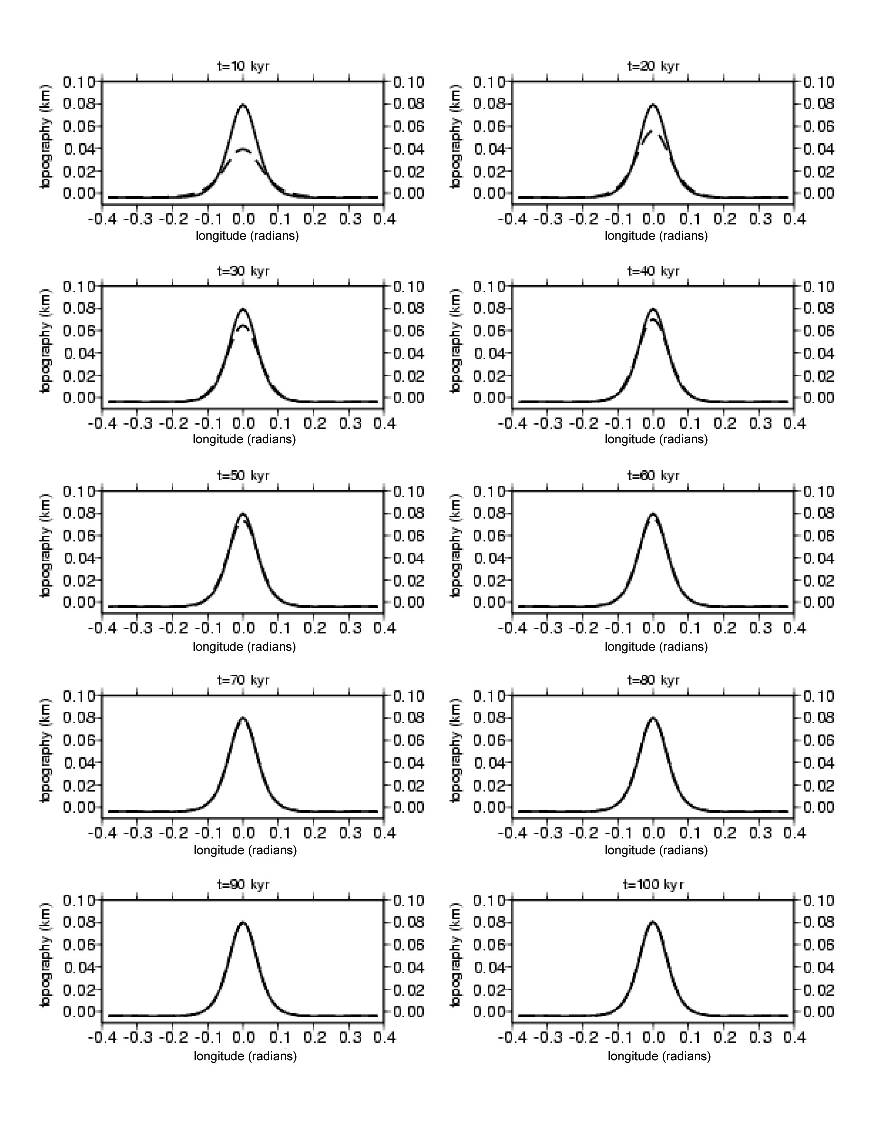
\includegraphics[scale=0.8]{graphics/cookbook6.pdf}
\par\end{centering}

\caption{\label{fig:Cookbook-6.-Graphs}Cookbook 6: Graphs of topography profiles. }
\end{figure}

\par\end{center}

\newpage{}


\section{Cookbook 7: Thermo-Chemical Convection}


\subsection{Problem}

This example solves for thermo-chemical convection within a full spherical
shell domain. Composition heterogeneity exists in the Earth mantle.
The density anomalies due to the composition heterogeneity, as well
as due to the thermal heterogeneity, drive the convection flow. 


\subsection{Solution}

You will use \texttt{cookbook7.cfg}. Most of the parameters you have
encountered in previous cookbooks. The initial condition is the same
as in Cookbook 1, and the viscosity law is the same as in Cookbook
3. 

A large number of ASCII files will be output. In order to keep the
current directory tidy, the output files can be put in a subdirectory
\texttt{output/} by specifying
\begin{lyxcode}
datadir~=~output
\end{lyxcode}
Since you are interested in the composition field, the compostion
output should be enabled and some output files disabled:
\begin{lyxcode}
output\_optional~=~tracer,comp\_nd
\end{lyxcode}
The most important parameters are in the \texttt{CitcomS.solver.tracer}
section. Turn on the tracer module:
\begin{lyxcode}
tracer~=~1
\end{lyxcode}
The number of tracers and their initial location must be set. Here,
you specify \texttt{tracer\_ic\_method=0}. The tracers will be generated
pseudo-randomly, with a total number equal to 
\begin{lyxcode}
tracers\_per\_element$\times$\textrm{(total~number~of~finite~elements).}
\end{lyxcode}
If \texttt{tracer\_ic\_method=1}, all processors will read the location
(and flavors; see next paragraph) of the tracers from the same file
specified by \texttt{tracer\_file}. If \texttt{tracer\_ic\_method=2},
each processor will read the location (and flavors; see next paragraph)
of the tracers from the file specified by \texttt{datafile\_old} (in
the \texttt{CitcomS.solver} section) and \texttt{solution\_cycles\_init}
(in the \texttt{CitcomS.solver.ic} section). 
\begin{lyxcode}
tracer\_ic\_method~=~0~\\
tracers\_per\_element~=~20~\\
tracer\_file~=~tracer.dat
\end{lyxcode}
Each tracer can have a ``flavor'' attached to it. The meaning of the
flavor depends on the application. Here, the flavor indicates the
chemical species of the tracer. There are two flavors of tracers (\texttt{tracer\_flavors=2}).
A tracer of flavor 0 is of the ``normal,'' or ambient, chemical composition,
while a tracer of flavor 1 is of the ``anomalous'' chemical composition.
Because the tracers are automatically generated, you need to specify
how to assign the flavor to each tracer. If \texttt{ic\_method\_for\_flavors=0},
tracers above \texttt{z\_interface} are assigned to flavor 0, and
tracers below \texttt{z\_interface} to flavor 1.
\begin{lyxcode}
tracer\_flavors~=~2~\\
ic\_method\_for\_flavors~=~0~\\
z\_interface~=~0.7
\end{lyxcode}
The thermo-chemical convection module is turned on by
\begin{lyxcode}
chemical\_buoyancy~=~1
\end{lyxcode}
The composition field is determined by the ratio method (\texttt{buoy\_type=1})
\cite{Tackely King tracer ratio method}. The density anomaly of the
anomalous chemical composition is defined by $B=\Delta\rho_{ch}/\left(\rho_{0}\alpha_{0}\Delta T\right)$,
the buoyancy ratio. 
\begin{lyxcode}
buoy\_type~=~1~\\
buoyancy\_ratio~=~0.5
\end{lyxcode}
The code keeps track of the sum of the bulk composition. In a perfect
world, the sum of the bulk composition would not change with time.
But due to numerical issues, the sum of the bulk composition tends
to decrease with time. If \texttt{tracer\_ic\_method=2}, the code
will read in the location of the tracers, as well as the initial sum
of the bulk composition, from the previous run. 

The regular grid is an auxiliary grid that helps locate the tracers
\cite{McNamara Zhong Thermochemical}. The optimal grid spacing of
the regular grid depends on the size of the CitcomS mesh. A general
rule of thumb is that the grid spacing of the regular grid should
be less than $18/(nodex\times nprocx)$. These parameters are used
only in the full spherical version.
\begin{lyxcode}
regular\_grid\_deltheta~=~1.0~\\
regular\_grid\_delphi~=~1.0
\end{lyxcode}
If you encounter any error, look at the end of the tracer log files
(\texttt{cookbook7.tracer\_log.{*}}) for error messages.

You will use the conjugate gradient solver to solve the matrix equation
$\mathbf{A}x=b$ for $x$. The conjugate gradient solver is more efficient
than the multigrid solver (\texttt{Solver=multigrid}) for small problems
(e.g., less than 17$\times$17$\times$17 nodes per processor). The
desired accuracy and maximum iterations are set by \texttt{accuracy}
and \texttt{vlowstep}. For the Uzawa algorithm, the maximum iterations
are set by \texttt{piterations}. \texttt{Both vlowstep }and \texttt{piterations}
should be large integers, but you can experiment with a larger value
for \texttt{accuracy} to speed up the computation. 
\begin{lyxcode}
Solver~=~cgrad~\\
accuracy~=~1e-03~\\
vlowstep~=~1000~\\
piterations~=~1000
\end{lyxcode}

\subsubsection{Example: Thermo-Chemical Convection, \texttt{cookbook7.cfg}}
\begin{lyxcode}
{[}CitcomS{]}~\\
solver~=~full~\\
steps~=~15~~~~~~~~~~~~~~~~~;~number~of~time~steps~\\
~\\
{[}CitcomS.controller{]}~\\
monitoringFrequency~=~5~~~~;~how~often~outputs~are~created~\\
~\\
{[}CitcomS.solver{]}~\\
datadir~=~output~~~~~~~~~~~;~path~to~output~directory~\\
datafile~=~cookbook7~~~~~~~;~prefix~of~output~filenames~\\
rayleigh~=~1e7~\\
~\\
{[}CitcomS.solver.ic{]}~\\
num\_perturbations~=~1~\\
perturbl~=~3~\\
perturbm~=~2~\\
perturblayer~=~5~\\
perturbmag~=~0.05~\\
~\\
{[}CitcomS.solver.output{]}~\\
output\_optional~=~tracer,comp\_nd~\\
~\\
{[}CitcomS.solver.tracer{]}~\\
tracer~=~on~\\
tracer\_ic\_method~=~0~\\
tracers\_per\_element~=~20~\\
tracer\_file~=~tracer.dat~\\
~\\
tracer\_flavors~=~2~\\
ic\_method\_for\_flavors~=~0~\\
z\_interface~=~0.7~\\
~\\
chemical\_buoyancy~=~1~\\
buoy\_type~=~1~\\
buoyancy\_ratio~=~0.5~\\
~\\
regular\_grid\_deltheta~=~1.0~\\
regular\_grid\_delphi~=~1.0~\\
~\\
{[}CitcomS.solver.vsolver{]}~\\
Solver~=~cgrad~\\
accuracy~=~1e-04~\\
vlowstep~=~1000~\\
piterations~=~1000~\\
~\\
\#~Assign~the~viscosities.~\\
{[}CitcomS.solver.visc{]}~\\
VISC\_UPDATE~=~on~\\
num\_mat~=~4~\\
visc0~=~1,1,1,1~\\
TDEPV~=~on~\\
rheol~=~4~\\
viscE~=~0.2,0.2,0.2,0.2~\\
viscT~=~0,0,0,0~\\
viscZ~=~0,0,0,0~\\
VMIN~=~on~\\
visc\_min~=~1.0~\\
VMAX~=~on~\\
visc\_max~=~100.0
\end{lyxcode}
\noindent \begin{center}
\begin{figure}[H]
\noindent \begin{centering}
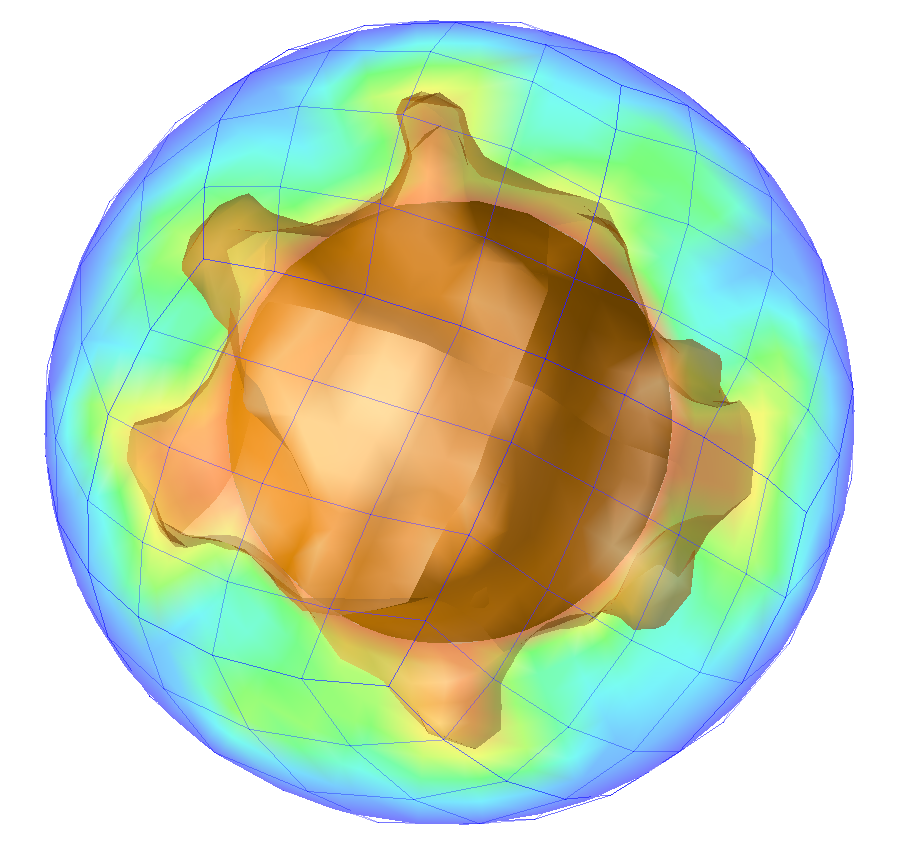
\includegraphics[width=0.3\paperwidth]{graphics/cookbook7.png}
\par\end{centering}

\caption{\label{fig:Cookbook-7:-The}Cookbook 7: The composition and velocity
field at the 15th step. The arrows are the velocity vectors. The composition
field is shown in an isosurface of 0.7 and in a cross section.}
\end{figure}

\par\end{center}


\subsection{Discussion}

When the model is running, it will output the progress of the run
to the screen. This line has information about the grid:
\begin{lyxcode}
Problem~has~9~x~9~x~9~nodes~per~cap,~6930~nodes~and~6144~elements~in~total
\end{lyxcode}
The following lines give the radial coordinate and reference density
of each nodes and their viscosity layer:
\begin{lyxcode}
~~~~nz~~~~~radius~~~~~~depth~~~~rho~~~~~~~~~~~~~~layer~\\
~~~~~~1~~~~0.550000~~~~0.450000~1.000000e+00~~~~~4~\\
~~~~~~2~~~~0.606250~~~~0.393750~1.000000e+00~~~~~4~\\
~~~~~~3~~~~0.662500~~~~0.337500~1.000000e+00~~~~~4~\\
~~~~~~4~~~~0.718750~~~~0.281250~1.000000e+00~~~~~4~\\
~~~~~~5~~~~0.775000~~~~0.225000~1.000000e+00~~~~~4~\\
~~~~~~6~~~~0.831250~~~~0.168750~1.000000e+00~~~~~4~\\
~~~~~~7~~~~0.887500~~~~0.112500~1.000000e+00~~~~~4~\\
~~~~~~8~~~~0.943750~~~~0.056250~1.000000e+00~~~~~2~\\
~~~~~~9~~~~1.000000~~~~0.000000~1.000000e+00~~~~~1
\end{lyxcode}
This line gives the perturbation parameters used to construct the
initial temperature:
\begin{lyxcode}
Initial~temperature~perturbation:~~layer=5~~mag=0.05~~l=3~~m=2~
\end{lyxcode}
This line gives the magnitude the right-hand side vector in Equation
\ref{eq:discrete momentum eqn}:
\begin{lyxcode}
Momentum~equation~force~2.207120371e+03
\end{lyxcode}
The following lines give the convergence progress of the Stokes solver,
where \texttt{v} is the volume averaged norm of velocity, \texttt{p}
is the volume averaged norm of pressure, \texttt{div/v} is the volume
averaged norm of $\nabla\cdot(\bar{\rho}v)$ divided by \texttt{v},
\texttt{dv/v} is the volume averaged norm of velocity change divided
by \texttt{v}, and \texttt{dp/p} is the volume averaged norm of pressure
change divided by \texttt{p}. The convergence of the Stokes solver
is achieved if either (1) \texttt{div/v }is less than\texttt{ accuracy}
or (2) both \texttt{dv/v} and \texttt{dp/p} are less than \texttt{accuracy}
for two consecutive iterations. In this example, the second condition
is met.
\begin{lyxcode}
(000)~~~7.0~s~v=1.470010e+02~p=0.000000e+00~div/v=5.37e+00~dv/v=1.00e+00~dp/p=1.00e+00~step~0~\\
$\vdots$~\\
(090)~151.3~s~v=1.012752e+02~p=1.304499e+04~div/v=5.54e-04~dv/v=1.84e-05~dp/p=9.20e-05~step~0~\\
(091)~151.8~s~v=1.012752e+02~p=1.304512e+04~div/v=5.66e-04~dv/v=2.07e-05~dp/p=7.45e-05~step~0~
\end{lyxcode}
This line gives the rotation angle and the angular coordinates of
rotation pole of the removed net angular momentum:
\begin{lyxcode}
Angular~momentum:~rot=9.917258e-02~tr=8.924735e+01~fr=1.083630e+02
\end{lyxcode}
These lines give the heat flux across the top and bottom surfaces:
\begin{lyxcode}
surface~heat~flux=~2.227892~\\
bottom~heat~flux=~2.216542
\end{lyxcode}
The surface heat flux \texttt{$H_{surf}$} can be converted to the
Nusselt number \texttt{$Nu_{surf}$} by:

\begin{equation}
Nu_{surf}=H_{surf}\times(r_{outer}-r_{inner})\frac{r_{outer}}{r_{inner}}\label{eq:Nusselt number}
\end{equation}


The results for this problem are presented in Figure \ref{fig:Cookbook-7:-The}.
The buoyancy ratio in this model is too low to stabilize the chemical
layer. A few thermo-chemical plumes are rising from the lower mantle,
especially the ones at the 4, 6, 9, 10, and 12 o'clock directions.
The resolution of this model is fairly low. The composition isosurface
is slightly discontinuous across the cap boundary. A model of higher
resolution will not have this kind of artifact.

\newpage{}


\section{Cookbook 8: Compressible Steady-State Convection}


\subsection{Problem}

This example is a benchmark problem for compressible thermal convection.
The Stokes solver in CitcomS has been benchmarked and validated against
a semi-analytical solution. However, no analytical solution exists
for the benchmark on the energy equation solver, which is nonlinear.
The steady-state solution is usually used for the comparison with
other numerical solutions. 


\subsection{Solution}

This cookbook example will run for 10,000 time steps to reach steady
state. It will use 12 processors and take 1 to 2 days to finish on
a modern computer. At every 1,000th time-step interval, a checkpoint
for the internal state of the solver is saved.
\begin{lyxcode}
checkpointFrequency~=~1000
\end{lyxcode}
If the solver is interrupted before finishing the computation, one
can resume the computation from the checkpointed state. To shorten
the computation time, a checkpoint at the 9,000th time step (\texttt{CitcomS-cookbook8-
restart.tar.gz}) is provided at CIG's CitcomS web page \url{geodynamics.org/cig/software/packages/mc/citcoms}.
(Note that the checkpoint files are produced by an x86 machine and
may not be usable by other types of machines, e.g., PowerPC.) To resume
the computation from the 9,000th time-step checkpoint, untar the package
in the \texttt{examples/Cookbook8/} directory and set these parameters:
\begin{lyxcode}
{[}CitcomS.solver.ic{]}~\\
restart~=~on~\\
solution\_cycles\_init~=~9000
\end{lyxcode}
If you restart from the checkpoint, the computation will resume from
the 9,000th time-step. Note that the \texttt{coord} files are only
output at the 0th time-step, so you will need to run the model without
restarting for one time-step to get the \texttt{coord} files.

A compressible convection model has four dimensionless numbers: the
Rayleigh number, the dissipation number, the Gruneisen parameter $\gamma=\alpha_{0}K_{S0}/\rho_{0}c_{P0}$,
and the non-dimensionalized absolute surface temperature, which are
defined in Section \ref{sec:Governing-Equations}. The Rayleigh number
of CitcomS is scaled by the radius of the Earth. If scaled to the
thickness of the mantle, the effective Rayleigh number is $7\times10{}^{3}$
($=7.68175583\times10{}^{4}\times(r_{outer}-r_{inner})^{3}$). Similarily,
the effective dissipation number is 0.275 ($=0.5\times(r_{outer}-r_{inner})$).
Under these non-dimensional numbers, the convection is of low vigor
and low compressibility.
\begin{lyxcode}
rayleigh~=~7.68175583e4~\\
dissipation\_number~=~0.5~\\
gruneisen~=~1.25~\\
surfaceT~=~0.1
\end{lyxcode}
Since we are going to use the multigrid solver, the grid size is specified
by:
\begin{lyxcode}
nodex~=~33~\\
nodey~=~33~\\
nodez~=~33~\\
levels~=~5
\end{lyxcode}
The additional parameter \texttt{levels} specifies the nested levels
of multigrid units and is subjected to the following constraint: 
\begin{equation}
\mathrm{nodex}=1+\mathrm{nprocx}\times\mathrm{mgunitx}\times2^{levels-1}\label{eq:mgunit}
\end{equation}
where \texttt{mgunitx} must be an integer. In the pure C version,
\texttt{mgunitx} is an input parameter.

If \texttt{reference\_state=}1, then constant gravity, heat capacity,
thermal expansivity, and $\rho_{r}=exp\left(\frac{D_{i}}{\gamma}(1-r)\right)$
are used as the reference state. If \texttt{reference\_state=}0, the
reference state is read from a file \texttt{refstate\_file}. See Appendix
\ref{cha:Appendix-A:-Input} for the file format.
\begin{lyxcode}
reference\_state~=~1~\\
refstate\_file~=~ref.dat
\end{lyxcode}
We are interested in the geoid, dynamic topography, and heat flux.
The dynamic topography and heat flux are computed on the surface grids.
The geoid is computed in the spherical harmonics, with a maximal degree
of \texttt{20}. 
\begin{lyxcode}
output\_optional~=~geoid,surf,botm~\\
output\_ll\_max~=~20
\end{lyxcode}
The initial temperature is a conductive profile with a single spherical
harmonic perturbation. The perturbation is located at mid-depth and
is defined as: 
\[
mag\times\sin\left(\frac{(r-r_{in})\pi}{r_{out}-r_{in}}\right)\left(\sin(m\phi)+\cos(m\phi)\right)P_{lm}(\cos\theta)
\]

\begin{lyxcode}
tic\_method~=~3~\\
num\_perturbations~=~1~\\
perturbl~=~3~\\
perturbm~=~2~\\
perturblayer~=~17~\\
perturbmag~=~0.01
\end{lyxcode}
You will need the output of dynamic topography and the geoid. The
dynamics topography will be computed by the Consistent Boundary Flux
(CBF) method, and the effect of self-gravitation is included in the
geoid. The maximum spherical harmonics degree for the geoid is 20.
\begin{lyxcode}
output\_optional~=~geoid,surf,botm~\\
use\_cbf\_topo~=~on~\\
self\_gravitation~=~on~\\
output\_ll\_max~=~20
\end{lyxcode}
Various parameters tune the performance of the solver. The maximum
size of each time step is determined dynamically by the Courant criterion.
To enhance the stability of the energy equation solver, you will only
use three quarters of the maximum Courant time-step size.
\begin{lyxcode}
finetunedt~=~0.75
\end{lyxcode}
You will use the multigrid solver to solve the matrix equation $\mathbf{A}x=b$
for $x$. The multigrid solver is more efficient than the conjugate
gradient solver (\texttt{Solver=cgrad}) for larger problems (e.g.,
more than 17$\times$17$\times$17 nodes per processor). Several parameters
control the behavior of the multigrid solver: \texttt{mg\_cycle=1}
for the V cycle and \texttt{2} for the W cycle; \texttt{down\_heavy}
and \texttt{up\_heavy} are the number of smoothing cycles for downward/upward
smoothing; \texttt{vlowstep} and \texttt{vhighstep} are the number
of smoothing passes at lowest/highest levels; and \texttt{max\_mg\_cycles}
is the maximum number of multigrid cycles per solve. All these parameters
should be small integers.
\begin{lyxcode}
Solver~=~multigrid~\\
mg\_cycle~=~1~\\
down\_heavy~=~2~\\
up\_heavy~=~2~\\
vlowstep~=~20~\\
vhighstep~=~2~\\
max\_mg\_cycles~=~50
\end{lyxcode}
The following parameter turn on the pre-conditioner for the matrix
equation solver (either multigrid or conjugate gradient).
\begin{lyxcode}
precond~=~on
\end{lyxcode}
The stiffness matrix uses augmented Lagrangian formulation to improve
the convergence for large viscosity variations \cite{Moresi/Zhong/Gurnis The accuracy}.
These parameters specify whether to enable the formulation and how
much weight to use for the formulation.
\begin{lyxcode}
aug\_lagr~=~on~\\
aug\_number~=~2.0e3
\end{lyxcode}
The discrete Stokes equations \ref{eq:discrete continuite eqn} and
\ref{eq:discrete momentum eqn} are solved using the Uzawa algorithm,
which iteratively updates the pressure and velocity solutions. Three
variations of the Uzawa algorithm are used in CitcomS, one for the
incompressible case, and the other two for the compressible case.
One parameter, \texttt{piterations,} common to the three variations,
specifies the maximum number of iterations and the desired residual
level for the continuity equation \ref{eq:discrete continuite eqn}.
Sometimes, larger value of \texttt{piterations} is required for convergence
if complicated velocity boundary conditions are used.
\begin{lyxcode}
piterations~=~375
\end{lyxcode}
For the compressible case, two choices of the Uzawa algorithm are
available. If \texttt{uzawa=cg}, the algorithm described in Equation
\ref{eq:iter-cg} is used. In this case, an additional parameter controls
the maximum number of outer iterations. 
\begin{lyxcode}
uzawa~=~cg~\\
compress\_iter\_maxstep~=~100
\end{lyxcode}
If \texttt{uzawa=bicg}, the algorithm described in Equation \ref{eq:bicg}
is used, and no additional parameter is needed.

The overall accuracy of the velocity solver is controlled by a single
parameter. The solver is converged if the residuals of Equation \ref{eq:discrete continuite eqn}
and \ref{eq:discrete momentum eqn} both are smaller than \texttt{accuracy},
or if the changes in the velocity and pressure both are smaller than
\texttt{accuracy} for the last two iterations.
\begin{lyxcode}
accuracy~=~0.001
\end{lyxcode}
Finally, the net angular momentum of the velocity solution is removed.
The net angular momentum and rigid body rotation are unconstrained
by the Stokes equations, if free-slip boundary conditions are used
for the top and bottom boundaries in a full spherical model. That
is, you can add an arbitrary amount of rotation to the velocity solution,
and the resultant velocity is still a valid solution of the Stokes
equations. Since no external torque is applied to the mantle in free-slip
boundary conditions, the angular momentum must be constant in time.
Enforcing the angular momentum to be zero by removing it from the
velocity solution is often desirable. 
\begin{lyxcode}
remove\_rigid\_rotation~=~off~\\
remove\_angular\_momentum~=~on
\end{lyxcode}
However, for models with imposed plate velocity, it is advisable to
turn off both \texttt{remove\_rigid\_rotation} and \texttt{remove\_angular\_momentum}.


\subsubsection{Example: Compressible Steady-State Convection, cookbook8.cfg}
\begin{lyxcode}
\#~Cookbook~8:~Compressible~Model~and~Checkpointing~\\
~\\
{[}CitcomS{]}~\\
solver~=~full~\\
steps~=~10000~\\
~\\
{[}CitcomS.controller{]}~\\
monitoringFrequency~=~1000~\\
checkpointFrequency~=~1000~\\
~\\
{[}CitcomS.solver{]}~\\
datadir~=~output~\\
datafile~=~cookbook8~\\
datadir\_old~=~restart~\\
datafile\_old~=~cookbook8~\\
~\\
rayleigh~=~7.68175583e4~\\
dissipation\_number~=~0.5~\\
gruneisen~=~1.25~\\
surfaceT~=~0.1~\\
~\\
{[}CitcomS.solver.mesher{]}~\\
nodex~=~33~\\
nodey~=~33~\\
nodez~=~33~\\
levels~=~5~\\
~\\
coor~=~1~\\
coor\_file~=~coord.dat~\\
~\\
{[}CitcomS.solver.param{]}~\\
reference\_state~=~1~\\
refstate\_file~=~ref.dat~\\
~\\
{[}CitcomS.solver.output{]}~\\
output\_optional~=~geoid,surf,botm~\\
use\_cbf\_topo~=~on~\\
self\_gravitation~=~on~\\
output\_ll\_max~=~20~\\
~\\
{[}CitcomS.solver.ic{]}~\\
tic\_method~=~3~\\
num\_perturbations~=~1~\\
perturbl~=~3~\\
perturbm~=~2~\\
perturblayer~=~17~\\
perturbmag~=~0.01~\\
~\\
restart~=~off~\\
solution\_cycles\_init~=~9000~\\
~\\
{[}CitcomS.solver.visc{]}~\\
VISC\_UPDATE~=~on~\\
visc\_smooth\_method~=~1~\\
~\\
TDEPV~=~on~\\
rheol~=~1~\\
num\_mat~=~4~\\
viscE~=~2.99573,2.99573,2.99573,2.99573~\\
viscT~=~0.5,0.5,0.5,0.5~\\
visc0~=~1,1,1,1~\\
~\\
VMIN~=~on~\\
visc\_min~=~0.001~\\
VMAX~=~on~\\
visc\_max~=~1e+06~\\
~\\
{[}CitcomS.solver.tsolver{]}~\\
finetunedt~=~0.75~\\
~\\
{[}CitcomS.solver.vsolver{]}~\\
uzawa~=~cg~\\
Solver~=~multigrid~\\
mg\_cycle~=~1~\\
down\_heavy~=~2~\\
up\_heavy~=~2~\\
vlowstep~=~20~\\
vhighstep~=~2~\\
max\_mg\_cycles~=~50~\\
~\\
aug\_lagr~=~on~\\
aug\_number~=~2.0e3~\\
precond~=~on~\\
~\\
piterations~=~375~\\
accuracy~=~0.001~\\
compress\_iter\_maxstep~=~100~\\
~\\
remove\_rigid\_rotation~=~off~\\
remove\_angular\_momentum~=~on
\end{lyxcode}

\subsection{Discussion}

The results for this problem are presented in Figure \ref{fig:Cookbook-8}.
A tetrahedral symmetric pattern is developed for the convection. The
surface heat flux $H_{surf}$ at the steady state is 3.892, and the
bottom heat flux $H_{botm}$ is 12.817. The heat flux imbalance ($H_{botm}r_{inner}^{2}/H_{surf}r_{outer}^{2}-1$)
is -0.38\%. The Nussult number, converted from the surface heat flux
by Equation \ref{eq:Nusselt number}, is 3.182. The total viscous
heating is 7.68991, and the total adiabatic cooling is 7.71719. Under
a steady state, these two terms should be exactly balanced.

The geoid is output as spherical harmonic coefficients. A post-processing
program is provided to project the geoid coefficients to a regular
(longitude, latitude) grid. To use a regular grid of $1^{\circ}$
spacing, run this command:
\begin{lyxcode}
\$~visual/project\_geoid~cookbook8.geoid.0.10000~geoid.xyz~361~181
\end{lyxcode}
It will generate a file \texttt{geoid.xyz}. There are 3 columns in
the file, which are (longitude, latitude, geoid). The geoid is in
a unit of meters. Several dimensional constants are required for the
geoid computation. These constants have sensible default values (in
SI units) for the Earth. Note that the temperature drop from the core-mantle
boundary to the surface ($\Delta T$ in Equation \ref{eq:T dim})
is derived from these constants and the Rayleigh number.
\begin{lyxcode}
{[}CitcomS.solver.const{]}~\\
radius=6.371e+06~\\
density=3340~\\
thermdiff=1e-06~\\
gravacc=9.81~\\
thermexp=3e-05~\\
refvisc=1e+21~\\
cp=1200~\\
density\_above=1030~\\
density\_below=6600~
\end{lyxcode}
\begin{figure}[H]
\begin{centering}
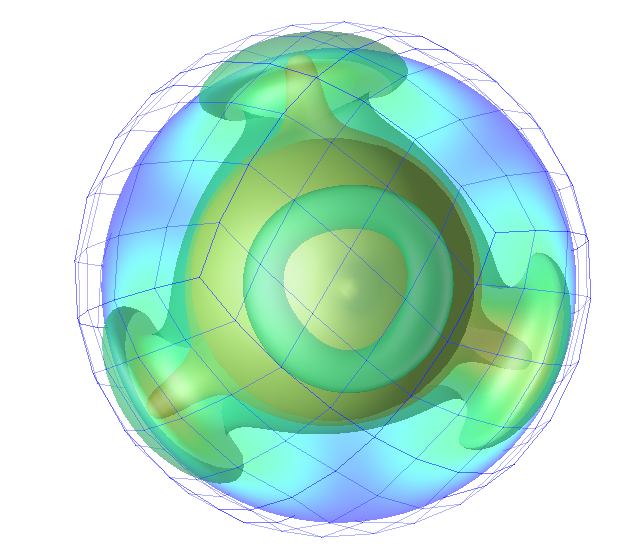
\includegraphics[scale=0.75]{graphics/cookbook8.png}
\par\end{centering}

\caption{\label{fig:Cookbook-8}Cookbook 8: The steady state temperature field
at the 10,000th time step. A tetrahedral symmetric convection pattern
is developed. Two temperature isosurfaces of 0.4 and 0.8 are shown. }
\end{figure}


\newpage{}


\section{Cookbook 9: Nested Solver Coupling for Ridge-Plume Interaction}

To run this cookbook, you need to install the Exchanger package. See
Section \vref{sec:Exchanger-Configuration-(Optional)} for installation
instructions.


\subsection{Problem}

In order to model the interaction between a segment of a mid-ocean
ridge and a plume, a small grid spacing is required to resolve the
thin plume conduit and the flow near the ridge. In addition, the plume
must be placed sufficiently away from the sidewalls to avoid possible
boundary effects. Satisfying both of these requirements in a model
entails a long computation time. Using solver coupling, a high-resolution
model with a smaller domain can be nested within a low-resolution
model, and the computation time significantly reduced. 


\subsection{Solution}

You will use two solvers in the model. A special command-line option
is required for a coupled model. Type the following command to run
this cookbook example:
\begin{lyxcode}
\$~citcoms~-{}-coupled~cookbook9.cfg
\end{lyxcode}
The embedded solver (esolver) is nested within the domain of the containing
solver (csolver). The velocity boundary conditions of the esolver
are fixed normal velocity and shear stress, whose values are received
from the esolver. The containing solver can be either a full CitcomS
solver or a regional one. The embedded solver can only be a regional
one. Both solvers are instances of a regional CitcomS solver in the
cookbook example. 
\begin{lyxcode}
csolver~=~regional~~~~~~;~containing~solver~\\
esolver~=~regional~~~~~~;~embedded~solver
\end{lyxcode}
You will use four processors for this model. Each solver will use
two processors. The rank-0 and rank-1 processors will be assigned
to the csolver, and the rank-2 and rank-3 processors will be assigned
to the esolver.
\begin{lyxcode}
{[}CitcomS.layout{]}~\\
containing\_group~=~{[}0-1{]}~\\
embedded\_group~=~{[}2-3{]}
\end{lyxcode}
The procedure for the nested solver coupling is described elsewhere
\cite{Tan et al GeoFramework Part I} and only briefly described below:
\begin{enumerate}
\item The containing solver solves the velocity and computes its time-step
size $dt_{c}$.
\item The containing solver interpolates the velocity, stress and temperature
onto the boundary of the embedded model.
\item The embedded model solves the velocity and temperature, using the
boundary conditions from step 2, with a time-step size $dt_{e}$;
$dt_{e}$ is always smaller than $dt_{c}$.
\item Step 3 is repeated until the sum of $dt_{e}$ is equal to $dt_{c}$.
\item Optionally (if \texttt{two\_way\_communication} is \texttt{on}), the
containing solver updates its temperature according to the embedded
solver's temperature.
\item The containing solver solves the temperature with a time-step size
$dt_{c}$.
\item The entire process repeats beginning at step 1.
\end{enumerate}
The two solver processes are separated and only communicate through
the couplers, which in turn use the exchanger package to pass messages.
The containing coupler and controller (ccoupler and ccontroller) are
associated with the csolver, and the embedded coupler and controller
(ecoupler and econtroller) with the esolver. Each solver will track
its own number of time steps. The esolver has a smaller time-step
size and, hence, a larger number of time steps. The model will finish
when either of the solvers reaches the 200th time step. The csolver
will output for every 2 steps and the esolver for every 10 steps.
Additional output will occur when the embedded solver is at procedure
4 above.
\begin{lyxcode}
{[}CitcomS{]}~\\
steps~=~200~\\
~\\
{[}CitcomS.ccontroller{]}~\\
monitoringFrequency~=~2~\\
~\\
{[}CitcomS.econtroller{]}~\\
monitoringFrequency~=~10
\end{lyxcode}
A few parameters must be identical for the ccoupler and ecoupler.
You will use two-way communication, which enables the ecoupler to
send temperature information to the ccoupler. Otherwise the communication
is one way, ccoupler to ecoupler only, and the csolver is not affected
by the esolver.
\begin{lyxcode}
two\_way\_communication~=~on
\end{lyxcode}
There is an option to exchange initial temperature, which could ensure
that the initial temperature field of both solvers is consistent.
The initial temperature field is read from velo files, which already
contain consistent temperature fields and don't need to exchange that
information again. 
\begin{lyxcode}
exchange\_initial\_temperature~=~off
\end{lyxcode}
A good initial guess of pressure field can speed up the convergence
of the iterative Stokes solver. We will use the pressure solution
of the containing solver as the initial guess of pressure of the embedded
solver.
\begin{lyxcode}
exchange\_pressure~=~on
\end{lyxcode}
Three additional parameters are for the ecoupler only. The following
two parameters specify whether the top and bottom boundary of the
esolver will be imposed with the velocity and temperature from the
csolver. For models with prescribed top or bottom boundary conditions,
you can turn on these two parameters:
\begin{lyxcode}
exclude\_top~=~off~\\
exclude\_bottom~=~off
\end{lyxcode}
The next parameter deserves a little more explanation. The continuity
equation \ref{eq:conservation of mass} can be rearranged according
to Gauss's divergence theorem to become:
\begin{eqnarray}
\ointop_{surface\ area}\rho_{0}\overrightarrow{u}\cdot\overrightarrow{n}dA & = & 0\label{eq:gauss div}
\end{eqnarray}
This equation requires that the normal velocity $\overrightarrow{u}$
imposed on the embedded solver must have zero outflow. Due to finite
accuracy of the containing solver and the interpolation process, the
normal velocity received by the embedded solver might not have zero
outflow, which could cause a convergence problem in the embedded solver.
One can amend the received normal velocity slightly to satisfy Equation
\ref{eq:gauss div} by setting:
\begin{lyxcode}
amending\_outflow~=~on
\end{lyxcode}
Without turning on \texttt{side\_sbcs}, the model will fail to run.
\begin{lyxcode}
{[}CitcomS.esolver.bc{]}~\\
side\_sbcs~=~on
\end{lyxcode}
Plate motion is imposed on top of the esolver, which has a mid-ocean
ridge with a 5 cm/yr half-spreading rate. A transform fault cuts through
the ridge. Setting \texttt{start\_age} to 0, the plate motion is read
from the file \texttt{velocity/bvel.dat0} and will be constant in
time.
\begin{lyxcode}
{[}CitcomS.csolver.bc{]}~\\
topvbc~=~1~\\
~\\
{[}CitcomS.csolver.param{]}~\\
file\_vbcs~=~on~\\
vel\_bound\_file~=~velocity/bvel.dat~\\
start\_age~=~0
\end{lyxcode}
The domain of the csolver is bigger than that of the esolver. The
radial dimension of the esolver will shrink slightly with respect
to the csolver so that the domain of the esolver is completely inside
the domain of the csolver. The radial coordinates of the csolver is
refined near the top and bottom boundaries (\texttt{coor=2}), with
the lower 10\% of the mesh divided by 15\% of the nodes, the upper
10\% of the mesh divided by 20\% of the nodes, and the remaining 80\%
of the mesh divided by 75\% of the nodes. 

Therefore, when setting the values of \texttt{coor\_refine} (see below),
be careful not to set the first or third value (in example below,
\texttt{0.1}) too low, or the second or fourth value (in example below,
\texttt{0.15} and \texttt{0.2}) too high. This can cause the mesh
size to change too rapidly across an element, which will generate
pronounced numerical artifacts in the temperature solver.
\begin{lyxcode}
{[}CitcomS.csolver.mesher{]}~\\
nprocz~=~2~\\
nodex~=~17~\\
nodey~=~17~\\
nodez~=~25~\\
radius\_outer~=~1.0~\\
radius\_inner~=~0.55~\\
theta\_min~=~1.171~\\
theta\_max~=~1.971~\\
fi\_min~=~0~\\
fi\_max~=~0.8~\\
coor~=~2~\\
coor\_refine~=~0.1,0.15,0.1,0.2~\\
~\\
{[}CitcomS.esolver.mesher{]}~\\
nprocz~=~2~\\
nodex~=~21~\\
nodey~=~21~\\
nodez~=~49~\\
radius\_outer~=~0.999~\\
radius\_inner~=~0.551~\\
theta\_min~=~1.421~\\
theta\_max~=~1.721~\\
fi\_min~=~0.25~\\
fi\_max~=~0.55
\end{lyxcode}
The temperature solver has several parameters to tune its behavior.
The temperature solver is turned on (\texttt{ADV}). A Lenardic-type
filter, which removes numerical artifacts while keeping total energy
conserved, is disabled (\texttt{filter\_temp}). The maximum temperature
can be monitored between time steps (\texttt{monitor\_max\_T}). If
the maximum temperature increases too much (> 5\%) between time steps,
the temperature solver will rerun with half time-step size. The time-step
size is usually determined dynamically according to Courant criterion
and is reduced by a fraction (\texttt{finetunedt}) to improve accuracy.
The time-step size can also be specified statically in \texttt{fixed\_timestep},
if \texttt{fixed\_timestep} is non-zero. The temperature solver uses
an explicit predictor-corrector algorithm. Using 0.5 for the predictor
(\texttt{adv\_gamma}) and 2 iterations for the corrector (\texttt{adv\_sub\_iterations}),
this algorithm is second-order accurate.
\begin{lyxcode}
ADV~=~on~\\
filter\_temp~=~off~\\
monitor\_max\_T~=~off~\\
finetunedt~=~0.9~\\
fixed\_timestep~=~0~\\
adv\_gamma~=~0.5~\\
adv\_sub\_iterations~=~2
\end{lyxcode}
The purpose of the csolver is to provide the proper boundary condition
for the esolver, and we don't need high accuracy for that. So we will
use low accuracy for the csolver and moderate accuracy for the esolver.
\begin{lyxcode}
{[}CitcomS.csolver.vsolver{]}~\\
accuracy~=~2e-2~\\
~\\
{[}CitcomS.esolver.vsolver{]}~\\
accuracy~=~1e-3~\\

\end{lyxcode}

\subsubsection{Example: Nested Solver Coupling for Ridge-Plume Interaction, cookbook9.cfg}
\begin{lyxcode}
\#~Cookbook~9:~Nested~Solver~Coupling~for~Ridge-Plume~Interaction~\\
~\\
{[}CitcomS{]}~\\
steps~=~200~\\
csolver~=~regional~~~~~~;~containing~solver~\\
esolver~=~regional~~~~~~;~embedded~solver~\\
~\\
{[}CitcomS.ccoupler{]}~\\
two\_way\_communication~=~on~\\
exchange\_initial\_temperature~=~off~\\
exchange\_pressure~=~on~\\
~\\
{[}CitcomS.ecoupler{]}~\\
two\_way\_communication~=~on~\\
exchange\_initial\_temperature~=~off~\\
exchange\_pressure~=~on~\\
amending\_outflow~=~on~\\
exclude\_top~=~off~\\
exclude\_bottom~=~off~\\
~\\
\#~assigning~processors~to~csolver~and~esolver~\\
{[}CitcomS.layout{]}~\\
containing\_group~=~{[}0-1{]}~\\
embedded\_group~=~{[}2-3{]}~\\
~\\
{[}CitcomS.ccontroller{]}~\\
monitoringFrequency~=~2~\\
~\\
{[}CitcomS.econtroller{]}~\\
monitoringFrequency~=~10~\\
~\\
{[}CitcomS.csolver{]}~\\
datadir\_old~=~ic~\\
datafile\_old~=~cntn~\\
datadir~=~output~\\
datafile~=~cntn~\\
rayleigh~=~1e8~\\
~\\
{[}CitcomS.csolver.mesher{]}~\\
nprocz~=~2~\\
nodex~=~17~\\
nodey~=~17~\\
nodez~=~25~\\
radius\_outer~=~1.0~\\
radius\_inner~=~0.55~\\
theta\_min~=~1.171~\\
theta\_max~=~1.971~\\
fi\_min~=~0~\\
fi\_max~=~0.8~\\
coor~=~2~\\
coor\_refine~=~0.1,0.15,0.1,0.2~\\
~\\
{[}CitcomS.csolver.bc{]}~\\
topvbc~=~1~\\
~\\
{[}CitcomS.csolver.param{]}~\\
file\_vbcs~=~on~\\
vel\_bound\_file~=~velocity/bvel.dat~\\
start\_age~=~0~\\
~\\
{[}CitcomS.csolver.ic{]}~\\
tic\_method~=~-1~\\
solution\_cycles\_init~=~0~\\
~\\
{[}CitcomS.csolver.tsolver{]}~\\
ADV~=~on~\\
filter\_temp~=~off~\\
monitor\_max\_T~=~off~\\
finetunedt~=~0.9~\\
fixed\_timestep~=~0~\\
adv\_gamma~=~0.5~\\
adv\_sub\_iterations~=~2~\\
~\\
{[}CitcomS.csolver.vsolver{]}~\\
accuracy~=~2e-2~\\
~\\
{[}CitcomS.csolver.visc{]}~\\
VISC\_UPDATE~=~on~\\
num\_mat~=~4~\\
visc0~=~1,1,1,1~\\
TDEPV~=~on~\\
viscE~=~1.6,1.6,1.6,1.6~\\
viscT~=~0,0,0,0~\\
VMIN~=~on~\\
visc\_min~=~1.0~\\
VMAX~=~on~\\
visc\_max~=~100.0~\\
~\\
\#\#\#\#\#\#\#\#\#\#\#\#\#\#\#\#\#\#\#\#\#\#\#\#\#\#\#\#\#\#\#\#\#\#\#\#\#\#\#\#\#\#\#\#\#\#\#~\\
~\\
{[}CitcomS.esolver{]}~\\
datadir\_old~=~ic~\\
datafile\_old~=~embd~\\
datadir~=~output~\\
datafile~=~embd~\\
rayleigh~=~1e8~\\
~\\
{[}CitcomS.esolver.mesher{]}~\\
nprocz~=~2~\\
nodex~=~21~\\
nodey~=~21~\\
nodez~=~49~\\
radius\_outer~=~0.999~\\
radius\_inner~=~0.551~\\
theta\_min~=~1.421~\\
theta\_max~=~1.721~\\
fi\_min~=~0.25~\\
fi\_max~=~0.55~\\
~\\
{[}CitcomS.esolver.ic{]}~\\
tic\_method~=~-1~\\
solution\_cycles\_init~=~0~\\
~\\
{[}CitcomS.esolver.vsolver{]}~\\
accuracy~=~1e-3~\\
~\\
{[}CitcomS.esolver.tsolver{]}~\\
ADV~=~on~\\
filter\_temp~=~off~\\
monitor\_max\_T~=~off~\\
finetunedt~=~0.9~\\
fixed\_timestep~=~0~\\
adv\_gamma~=~0.5~\\
adv\_sub\_iterations~=~2~\\
~\\
{[}CitcomS.esolver.visc{]}~\\
VISC\_UPDATE~=~on~\\
num\_mat~=~4~\\
visc0~=~1,1,1,1~\\
TDEPV~=~on~\\
viscE~=~1.6,1.6,1.6,1.6~\\
viscT~=~0,0,0,0~\\
VMIN~=~on~\\
visc\_min~=~1.0~\\
VMAX~=~on~\\
visc\_max~=~100.0~\\
~\\
{[}CitcomS.esolver.bc{]}~\\
side\_sbcs~=~on
\end{lyxcode}

\subsection{Discussion}

The solution of this problem is presented in Figure \ref{fig:Cookbook-9}.
The plume head spreads below the lithosphere, and the plume conduit
is elongated in the ridge-parallel direction. The lithosphere subducts
at the left and right edges of the csolver. If the domain of the csolver
were bigger, the plume would be further away from the subducted slabs. 

\begin{figure}[H]
\begin{centering}
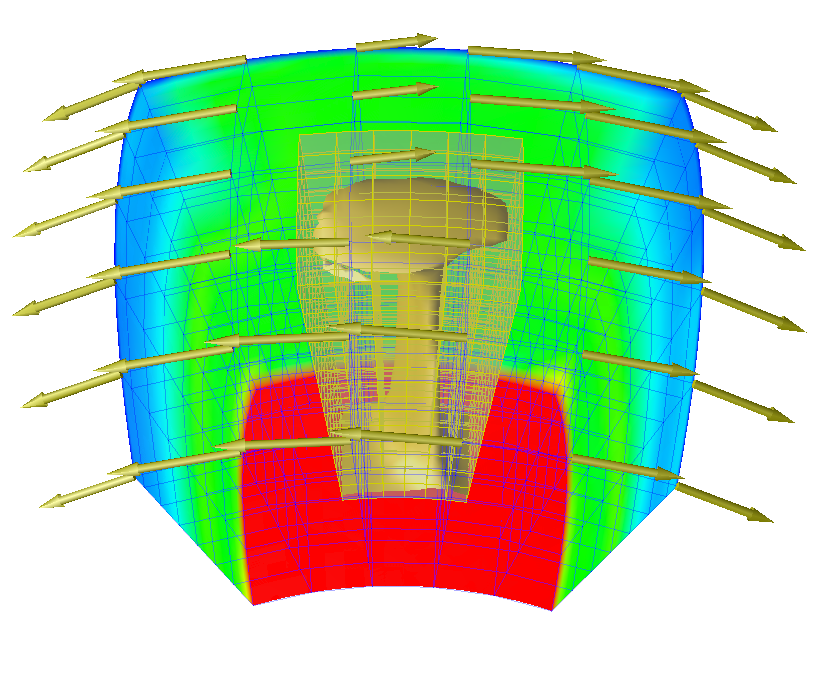
\includegraphics[width=0.6\paperwidth]{graphics/cookbook9.png}
\par\end{centering}

\caption{\label{fig:Cookbook-9}Cookbook 9: The plume head spreads below the
lithosphere, and the plume conduit is elongated in the ridge-parallel
direction. The temperature isosurface is at 0.8. The grid spacings
of both meshes are reduced approximately threefold for better visualization.}
\end{figure}


\newpage{}


\section{Cookbook 10: Synthetic Seismograms from Mantle Convection Models}


\subsection{Problem}

This example is a step-up of Cookbook \ref{fig:Cookbook-7:-The},
thermo-chemical convection within a full spherical shell domain. Composition
heterogeneity exists in the Earth mantle. The density anomalies due
to the composition heterogeneity, as well as due to the thermal heterogeneity,
drive the convection flow. The same composition heterogeneity causes
seismic velocity anomalies. The goal is to convert the mantle convection
models, with the aid of a mineral physics model, to seismic anomalies,
and then generate synthetic seismograms using SPECFEM3D\_GLOBE.


\subsection{Solution}

This cookbook uses CitcomS and SPECFEM3D\_GLOBE. SPECFEM3D\_GLOBE
is a spectral element code to simulate seismic wave propogation in
the global scale. To use SPECFEM3D\_GLOBE, you can either download
the code from this link \url{geodynamics.org/cig/software/packages/seismo/specfem3d-globe/}
and install it on your machine, which requires a Fortran 90 compiler
and a cluster, or you can go to CIG Seismology Web Portal \url{https://crust.geodynamics.org/portals/seismo/}
to launch a job, which only requires a browser. We will use the later
approach in the cookbook.


\subsubsection{Running CitcomS}

Most of the parameters are copied from Cookbook \ref{fig:Cookbook-7:-The}.
We will highlight a few differences. We use a higher Rayleigh number.
\begin{lyxcode}
rayleigh~=~1e9
\end{lyxcode}
The radius of the bottom surface is set to 0.546 in the cookbook,
which must be smaller than the CMB radius in SPECFEM3D\_GLOBE. (If
PREM is used as the 1D reference model in SPECFEM3D\_GLOBE, the CMB
radius is 0.5462.)
\begin{lyxcode}
radius\_inner~=~0.546~
\end{lyxcode}
We convert the temperature and composition fields to seismic velocities
using a mineral phyiscs model. Currently, there is only one model
implemented, based on the model of \textit{Trampert, Vacher, and Vlaar}\cite{Trampert mineral physics model 2001}.
In their paper, the (depth dependent) temperature and composition
derivatives of seismic velocities are given as polynomial coefficients.
Note that the paper has its own reference profile, and is only valid
between 1000 km < depth < 2600 km. We will extend the model to whole
mantle and use PREM as the reference profile. This clearly is over-stretching
the model, but we are using it for demonstration purposes.
\begin{lyxcode}
mineral\_physics\_model~=~3
\end{lyxcode}
We will output the converted density and seismic velocities for SPECFEM3D\_GLOBE
consumption. This option enables the binary seismic output (\texttt{{*}.seismic.{*}}
files), as well as other binary output (\texttt{{*}.domain} and \texttt{{*}.coord\_bin.{*}}
files) that SPECFEM3D\_GLOBE will read. The formats of these binary
files are provided in Appendix \ref{sec:Misc.-Binary-Output}.
\begin{lyxcode}
output\_optional~=~tracer,~comp\_nd,~seismic
\end{lyxcode}

\subsubsection{Example: Synthetic Seismograms from Mantle Convection Model, cookbook10.cfg}
\begin{lyxcode}
\#~Cookbook~10:~Synthetic~Seismograms~from~Mantle~Convection~Models

{[}CitcomS{]}

solver~=~full

steps~=~15~\\
~\\
{[}CitcomS.controller{]}

monitoringFrequency~=~5~\\
~\\
{[}CitcomS.solver{]}

datadir~=~output

datafile~=~cookbook10

rayleigh~=~1e9~\\
~\\
{[}CitcomS.solver.mesher{]}

radius\_inner~=~0.546~\\
~\\
{[}CitcomS.solver.ic{]}

num\_perturbations~=~1

perturbl~=~3

perturbm~=~2

perturblayer~=~5

perturbmag~=~0.05~\\
~\\
{[}CitcomS.solver.output{]}

output\_optional~=~tracer,comp\_nd,seismic~\\
~\\
{[}CitcomS.solver.param{]}

mineral\_physics\_model~=~3~\\
~\\
{[}CitcomS.solver.tracer{]}

tracer~=~on

tracer\_ic\_method~=~0

tracers\_per\_element~=~20

tracer\_file~=~tracer.dat~\\
~\\
tracer\_flavors~=~2

ic\_method\_for\_flavors~=~0

z\_interface~=~0.7~\\
~\\
chemical\_buoyancy~=~1

buoy\_type~=~1

buoyancy\_ratio~=~0.5~\\
~\\
regular\_grid\_deltheta~=~1.0

regular\_grid\_delphi~=~1.0~\\
~\\
{[}CitcomS.solver.vsolver{]}

Solver~=~cgrad

accuracy~=~1e-04

vlowstep~=~1000

piterations~=~1000~\\
~\\
\#~Assign~the~viscosities.

{[}CitcomS.solver.visc{]}

VISC\_UPDATE~=~on

num\_mat~=~4

visc0~=~1,1,1,1

TDEPV~=~on

rheol~=~4

viscE~=~0.2,0.2,0.2,0.2

viscT~=~0,0,0,0

viscZ~=~0,0,0,0

VMIN~=~on

visc\_min~=~1.0

VMAX~=~on

visc\_max~=~100.0
\end{lyxcode}

\subsubsection{Running SPECFEM3D\_GLOBE from CIG Seismology Web Portal}

Using your favorite browser, go to the CIG Seismology Web Portal \url{https://crust.geodynamics.org/portals/seismo/}.
Free registration is required to use the portal. Your initial account
has 10,000 SUs (CPU-hours) allocated. A short (20 minutes of seismograms),
low-resolution SPECFEM3D\_GLOBE run consumes about 450 SUs. A short,
high-resolution SPECFEM3D\_GLOBE run consumes about 1,000 SUs. Further
SUs can be allocated upon request.

After you login to the portal, take a few minutes to read the instructions
and familiarize yourself with the interface. You will see a toolbar
with big icons on the top and several grayed-out tabs below the toolbar.
The toolbar allows you to specify the earthquake source (\texttt{Events}),
the receivers (\texttt{Stations}), and simulation parameters (\texttt{3D
Parameters}), including the resolution (\texttt{Mesh}) and the seismic
velocity model for the crust and mantle (\texttt{3D Models}). In the
cookbook, we will upload the result of CitcomS as a 3D Model and upload
our own fictitious stations and event.

\begin{center}
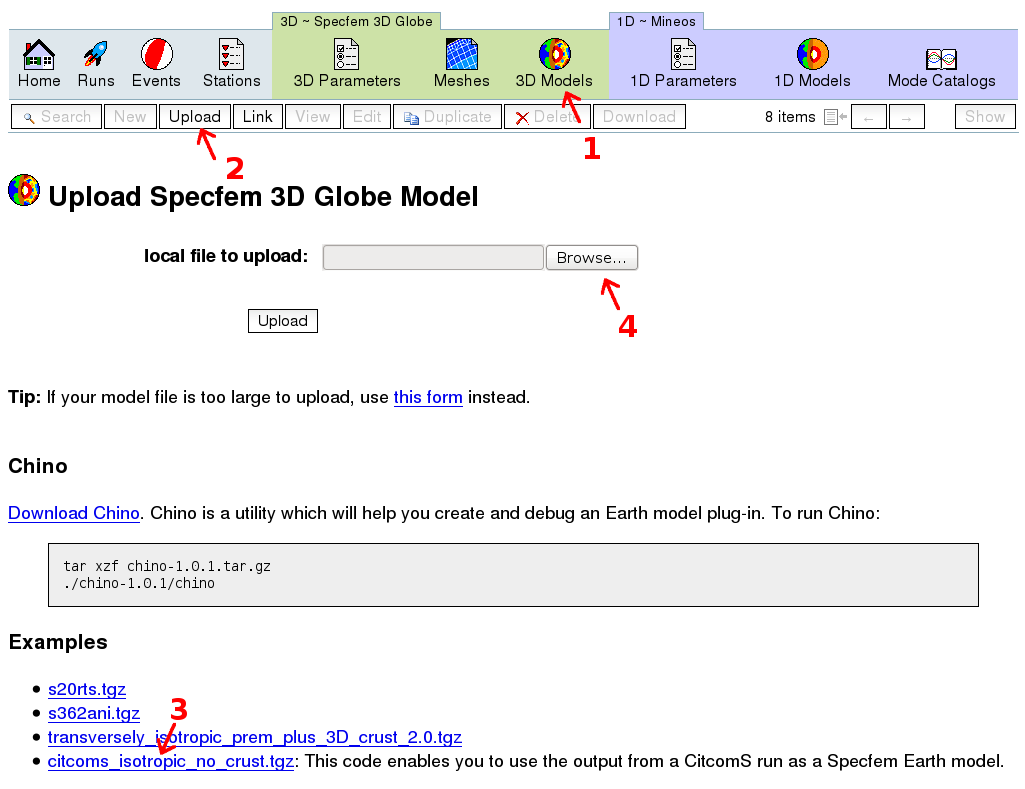
\includegraphics[scale=0.6]{graphics/portal-upload-a.png}
\par\end{center}

Click on the \texttt{3D Models} icon (1), and the \texttt{Upload}
tab (2), then click on the link \texttt{citcoms\_isotropic\_no\_crust.tgz}
(3) to download the tar file to your machine. The tar file you just
downloaded contains the code that reads CitcomS output and feeds the
seismic velocities to SPECFEM3D\_GLOBE. However, the tarball does
not contains the actual CitcomS output, which will be provided by
you later. As you might have guessed from the filename, the code will
generate an isotropic mantle without an overlay of a 3D crust, such
as the CRUST2.0 model. The 3D crust model obeys the continent-ocean
distribution of current Earth. Since our CitcomS model has no notation
on where is the Pacific and where is Asia, we do not want to impose
a 3D crust model. You can untar the file by running:
\begin{lyxcode}
\$~gunzip~-c~citcoms\_isotropic\_no\_crust.tgz~|~tar~xf~-
\end{lyxcode}
You will supply the CitcomS output to the code. Copy these CitcomS
output files \texttt{cookbook.domain}, \texttt{cookbook.coord\_bin.{*}},
and \texttt{cookbook.seismic.{*}.15} to the directory \texttt{citcoms\_isotropic\_no\_crust/shared/},
so that the content of the directory looks like:
\begin{lyxcode}
\$~ls~citcoms\_isotropic\_no\_crust/shared/

cookbook10.coord\_bin.0~~~cookbook10.seismic.0.15~

cookbook10.coord\_bin.1~~~cookbook10.seismic.10.15~

cookbook10.coord\_bin.10~~cookbook10.seismic.11.15~

cookbook10.coord\_bin.11~~cookbook10.seismic.1.15~

cookbook10.coord\_bin.2~~~cookbook10.seismic.2.15~

cookbook10.coord\_bin.3~~~cookbook10.seismic.3.15~

cookbook10.coord\_bin.4~~~cookbook10.seismic.4.15~

cookbook10.coord\_bin.5~~~cookbook10.seismic.5.15~

cookbook10.coord\_bin.6~~~cookbook10.seismic.6.15~

cookbook10.coord\_bin.7~~~cookbook10.seismic.7.15~

cookbook10.coord\_bin.8~~~cookbook10.seismic.8.15~

cookbook10.coord\_bin.9~~~cookbook10.seismic.9.15~

cookbook10.domain
\end{lyxcode}
These files contain the coordinate, density, and seismic velocities
data. We will need to tell SPECFEM3D\_GLOBE where to find the CitcomS
output. Edit the header file \texttt{citcoms\_isotropic\_no\_crust/citcoms\_parm.h}
to become:
\begin{lyxcode}
/{*}~filename~prefix~of~citcoms~output~{*}/

const~char~citcoms\_model\_filename\_base{[}{]}~=~\textquotedbl{}@THIS\_DIR@/shared/cookbook10\textquotedbl{};



/{*}~time~step~of~citcoms~output~{*}/

const~int~citcoms\_step~=~15;
\end{lyxcode}
The portal has a few conventions on where to put the data. First,
the magic string \texttt{@THIS\_DIR@} will be replaced by the absolute
path when the tar file is expanded by the portal. Second, the tar
file will be distributed to all computer nodes when portal launches
the job. Third, the subdirectory \texttt{shared/} is special such
that files in this directory will not be distributed to all computer
nodes. Data files of huge size should be put in this directory. You
might want to edit \texttt{citcoms\_isotropic\_no\_crust/description.txt}
to provide a description of your model. The text in this file will
be displayed on the portal. The final step before uploading is to
create a new tar file containing the code and data.
\begin{lyxcode}
\$~tar~cf~cookbook10.tar~citcoms\_isotropic\_no\_crust/

\$~gzip~cookbook10.tar
\end{lyxcode}
Now, you can upload the data by clicking on the \texttt{Browse} button
(4), choosing \texttt{cookbook10.tar.gz} from the resulting dialog
box, then clicking on the \texttt{Upload} button. After the portal
confirms that the upload is successful, click on the \texttt{3D Models}
icon again; you will see \texttt{cookbook10} is among the available
3D models.

\begin{center}
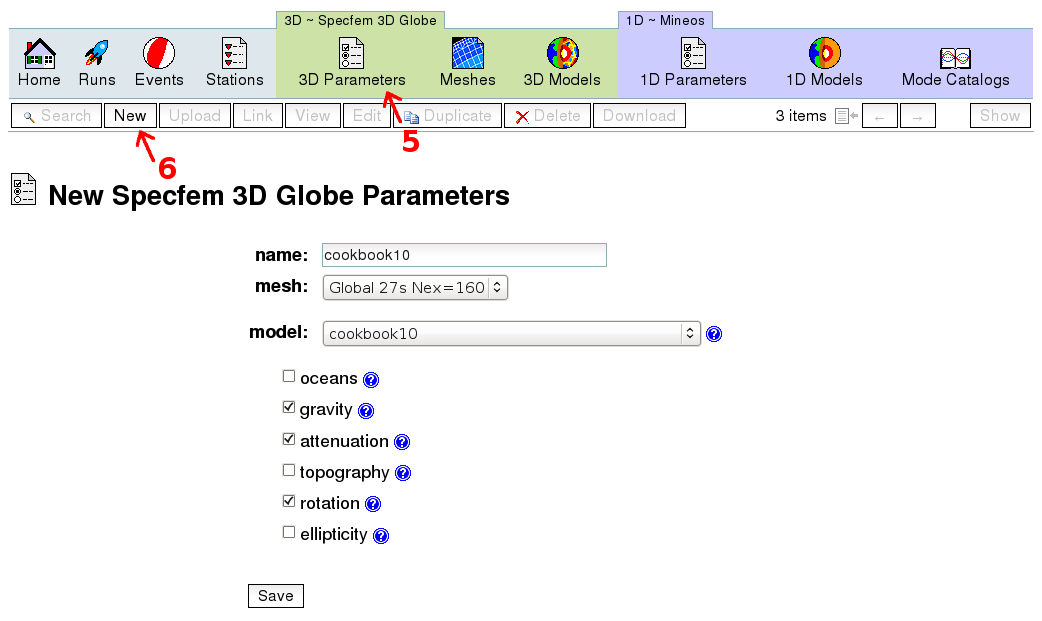
\includegraphics[scale=0.6]{graphics/portal-param-a.png}
\par\end{center}

You have to select a few parameters for a SPECFEM3D\_GLOBE run. Click
on the \texttt{3D Parameters} icon (5), the \texttt{New} tab (6),
select the parameters as shown in the figure above, and save the parameters
for later use. We will use a global mesh that is capable of resolving
seismic waves of 27 second period. Since CitcomS mesh is a perfect
sphere, you need to disable \texttt{topography} and \texttt{ellipticity}
to have a matching mesh in SPECFEM3D\_GLOBE. The \texttt{oceans} is
disabled because we don't have a 3D crust.

We will provide our own fictitious earthquake source and seismic stations.
The earthquake source is defined in \texttt{cmt-solution.cookbook10}
in the cookbook directory. The source is located at 15 km depth of
$0^{\circ}$N, $0^{\circ}$E. The half duration of the source is 0
second, which means a step function is used. Click on the \texttt{Events}
icon and the \texttt{upload} tab to upload the file \texttt{cmt-solution.cookbook10}.
The stations are defined in \texttt{stations.cookbook10} in the cookbook
directory. The stations are on the Equator and are 70 to 100 degrees
away from the source. Click on the \texttt{Stations} icon and the
\texttt{upload} tab to upload the file \texttt{stations.cookbook10}.

\begin{center}
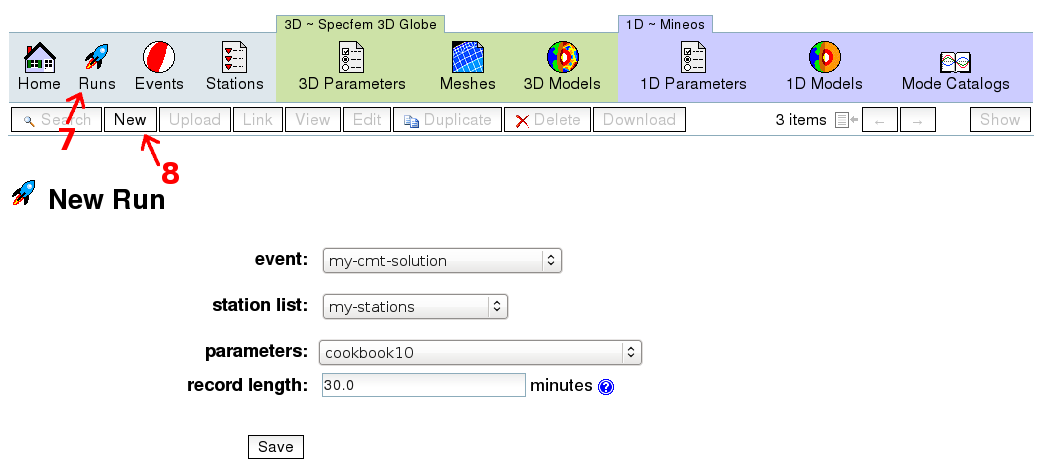
\includegraphics[scale=0.75]{graphics/portal-run-a.png}
\par\end{center}

Finally, we are ready to launch a SPECFEM3D\_GLOBE simulation. Click
on the \texttt{Runs} icon (7), then the \texttt{New} tab (8), and
select our recently uploaded event, stations and parameters. Set the
record length to 30 minutes, which will give us synthetic seismograms
of 30 minutes. Click the \texttt{Save} button to save the settings. 

\begin{center}
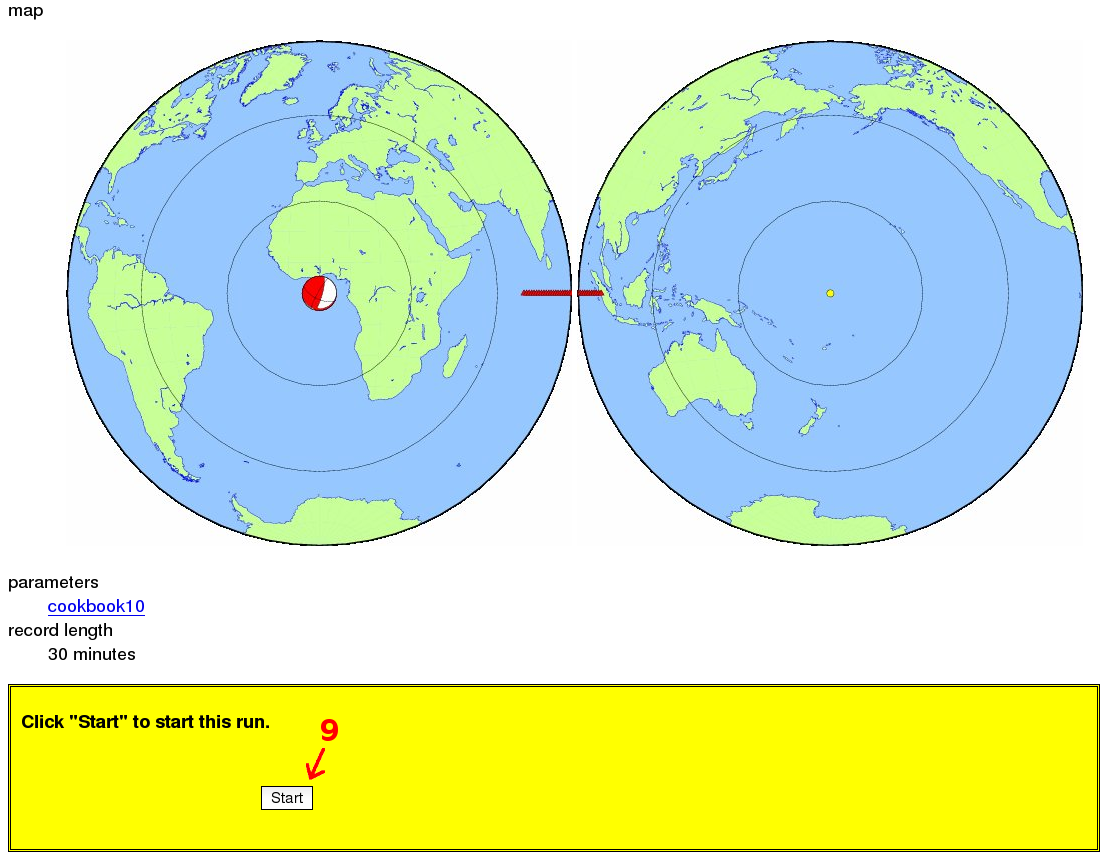
\includegraphics[scale=0.6]{graphics/portal-submit2-a.png}
\par\end{center}

You will be presented with a summary of the simulation settings, including
a map showing the location of the events and stations. After you have
reviewed all settings, scroll to the bottom of the page. Click on
the \texttt{Start} button. The request for the simulation is sent
to the TeraGrid supercomputing center. Your simulation will be waiting
in the queue and will be launched within several hours. You can log
off the portal for now.

\begin{center}
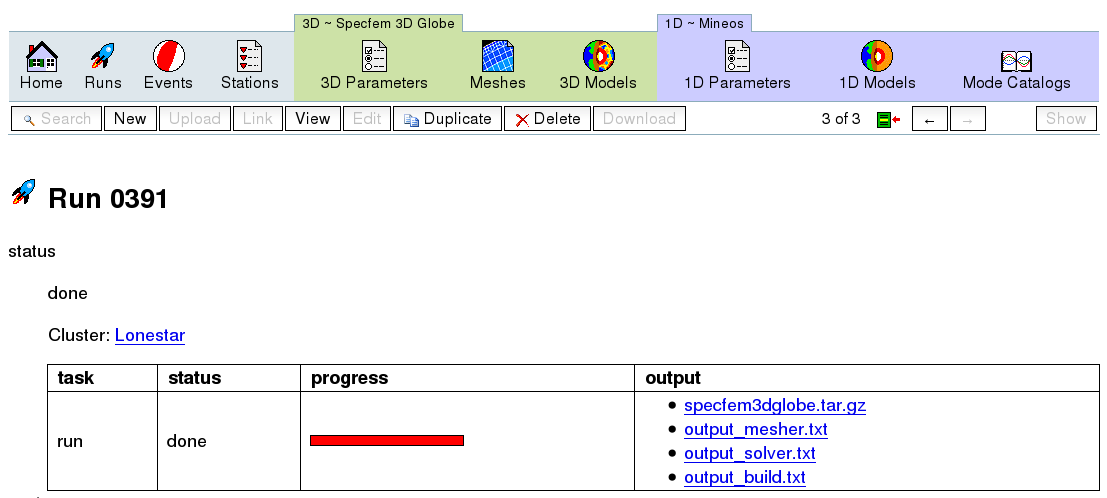
\includegraphics[scale=0.6]{graphics/portal-result.png}
\par\end{center}

When your simulation is finished, the portal will send you an e-mail
notification. Log in to the portal, click on the \texttt{Runs} icon,
where there is a list of finished and unfinished runs. Click on the
finished run, and you will see a list of output. Click on the \texttt{specfem3dglobe.tar.gz}
link to download the tar file. Expand the file:
\begin{lyxcode}
\$~gunzip~-c~specfem3dglobe.tar.gz~|~tar~xf~-
\end{lyxcode}
You will find the synthetic seismograms \texttt{{*}.sem.sac} in the
directory \texttt{OUTPUT\_FILES/}.


\subsection{Discussion}

The dimensional value of total temperature contrast across the mantle
is derived from the Rayleigh number in Equation \ref{eq:Ra, Rayleigh number}
and the dimensional parameters in the \texttt{{[}CitcomS.solver.const{]}}
section. In the very beginning of the simulation, the total temperature
contrast across the mantle is displayed on the screen. This value
will be used to scale the non-dimensional temperature when converting
the temperature anomaly to seismic velocities.
\begin{lyxcode}
Total~temperature~contrast~=~3934.055176~K
\end{lyxcode}
The event and stations are all on the equatorial plane. Figure \ref{fig:cookbook10}
shows the temperature field of the equatorial slice. A large warm
upwelling is beneath $60^{\circ}$E. We should be able to observe
its effect on delaying teleseismic waves in the $70^{\circ}$ to $90^{\circ}$
range.

\noindent \begin{center}
\begin{figure}[H]
\begin{centering}
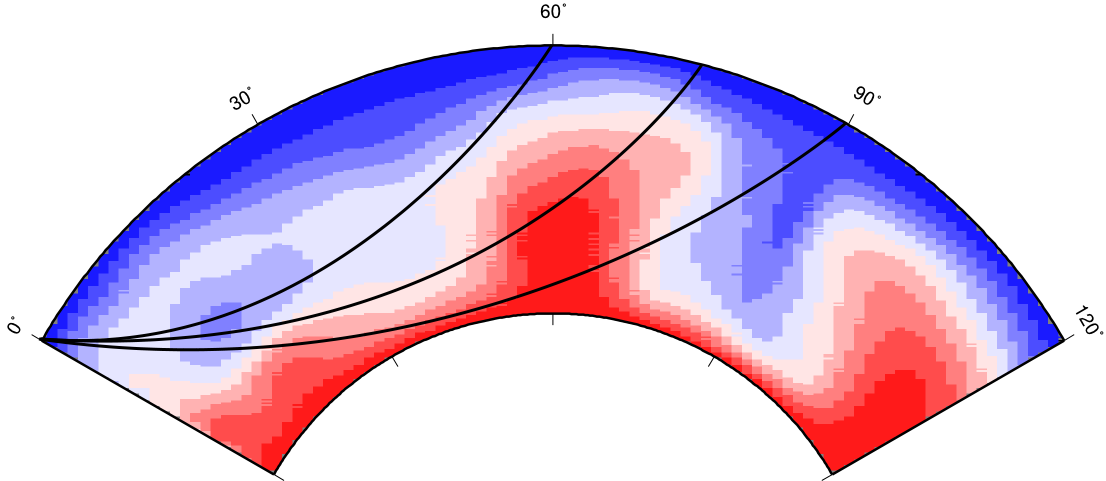
\includegraphics[scale=0.6]{graphics/cookbook10.png}
\par\end{centering}

\caption{\label{fig:cookbook10}The equatorial slice of temperature from the
CitcomS result. Three S wave paths probing the mantle are shown. }
\end{figure}

\par\end{center}

The synthetic seismograms need to be post-processed. The post-processing
programs we will use can be downloaded from the portal. Follow the
instructions on the portal to build the programs. We will band-pass
filter within the period of 30 and 500 seconds, and convolve the synthetics
with a gaussian source time function of 50 seconds half duration,
and append \texttt{conv} to the output filenames.
\begin{lyxcode}
\$~process\_syn.pl~-S~-t~30/500~-h~50~-x~conv~{*}.sac
\end{lyxcode}
Optionally, you can rotate the synthetics from East-North components
to Transversal-Radial components.
\begin{lyxcode}
\$~rotate.pl~{*}LHE{*}.conv
\end{lyxcode}

\part{Appendices}

\appendix

\chapter{\label{cha:Appendix-A:-Input}Input Parameters for CitcomS}


\section{Input Parameters Grouped by Functionality}

This section explains the meaning of the input parameters for CitcomS.
These parameters are grouped by their functionality. Parameters are
given with their default values.


\subsection{Parameters that Control Input Files}

\begin{tabular}{|>{\raggedright}p{1.85in}|>{\raggedright}p{4.25in}|}
\hline 
\texttt{\small{reference\_state=1}}~\\
\texttt{\small{refstate\_file=\textquotedbl{}refstate.dat\textquotedbl{}}} & If \texttt{\small{reference\_state}} is set to \texttt{\small{1}},
a simple reference state of $\rho_{r}=\exp\left((1-r)D_{i}/\gamma\right)$
is used, with constant gravity, thermal expansivity, and heat capacity.
If \texttt{\small{reference\_state}} is set to \texttt{\small{0}},
the reference state is read from a file \texttt{\small{refstate\_file}}\texttt{.} \tabularnewline
\hline 
\texttt{\small{mineral\_physics\_model=3}} & Using which mineral physics model to convert the seismic velocities.\tabularnewline
\hline 
\texttt{\small{file\_vbcs=off}}~\\
\texttt{\small{vel\_bound\_file=\textquotedbl{}bvel.dat\textquotedbl{}}} & If \texttt{\small{file\_vbcs}} is set to \texttt{\small{on}}, the
top surface velocity boundary conditions are read in from files which
have location and name specified by \texttt{\small{vel\_bound\_file}}\texttt{.}
Requires setting \texttt{\small{topvbc=1}} to take effect. If you
wish to have a uniform top surface velocity boundary condition or
some simple geometric pattern, then \texttt{\small{file\_vbcs}} should
be set to zero. \tabularnewline
\hline 
\texttt{\small{mat\_control=off}}\\
\texttt{\small{mat\_file=\textquotedbl{}mat.dat\textquotedbl{}}} & If \texttt{\small{mat\_control}} is set to \texttt{\small{on}}, then
the time- and positional-dependent viscosity factor is defined from
the files specified by \texttt{\small{mat\_file}}. These parameters
allow you to define the material group of each element (such as a
moving weak zone). Not working in this version.\tabularnewline
\hline 
\texttt{\small{lith\_age=off}}\\
\texttt{\small{lith\_age\_file=\textquotedbl{}age.dat\textquotedbl{}}}\\
\texttt{\small{lith\_age\_time=off}} & If \texttt{\small{lith\_age}} is set to \texttt{\small{on}}, then
the age of each surface nodes is read from the files specified by
\texttt{\small{lith\_age\_file}}. These parameters control the thermal
age of the top thermal boundary condition. If \texttt{\small{lith\_age\_time}}
is \texttt{\small{on}}, the files are time-dependent.\tabularnewline
\hline 
\end{tabular}


\subsection{Parameters that Control Output Files}

\noindent %
\begin{tabular}{|>{\raggedright}p{1.85in}|>{\raggedright}p{4.25in}|}
\hline 
\texttt{\small{output\_format=ascii}} & Choose the format and layout of the output files. Can be either \texttt{ascii},
\texttt{ascii-gz} or \texttt{hdf5}. If \texttt{ascii-gz} is chosen,
the code places gzipped files into \texttt{data\_dir}, and will put
all time-step output into subdirectories of \texttt{data\_dir}. The
same naming logic holds for reading old velo files.\tabularnewline
\hline 
\texttt{\small{output\_optional=\textquotedbl{}surf,}}~\\
\texttt{\small{botm,tracer\textquotedbl{}}} & Choose additional output, including \texttt{surf}, \texttt{botm},
\texttt{geoid}, \texttt{seismic}, \texttt{stress}, \texttt{pressure},
\texttt{connectivity}, \texttt{horiz\_avg, tracer, heating, comp\_el}
and\texttt{ comp\_nd}.\tabularnewline
\hline 
\texttt{\small{datadir=\textquotedbl{}.\textquotedbl{}}} & Controls the location of output files. \tabularnewline
\hline 
\texttt{\small{datafile=\textquotedbl{}regtest\textquotedbl{}}} & Controls the prefix of output file names such as \texttt{regtest.xxx}.
Cannot contain the ``\texttt{/}'' character if \texttt{output\_format=ascii}.\tabularnewline
\hline 
\texttt{\small{storage\_spacing=10}}\\
(in non-Pyre version)\\
or\\
\texttt{\small{monitoringFrequency=100}}\\
(in Pyre version) & Controls the interval between output files. CitcomS dynamically determines
the size of the time step; this means that you might not get an output
at the exact time required, but you can always get close depending
on how small this number is. Do not make this number too small since
outputs slow the code down and you may end up with an unmanageable
number of output files. \tabularnewline
\hline 
\texttt{\small{checkpointFrequency=100}} & The time-step interval between checkpoint output, which can be used
later to resume the computation.\tabularnewline
\hline 
\texttt{\small{output\_ll\_max=20}} & This parameter controls the maximum degree of spherical harmonics
coefficients for geoid output.\tabularnewline
\hline 
\texttt{self\_gravitation=off} & Considering the effect the self gravitation on the geoid or not.\tabularnewline
\hline 
\texttt{use\_cbf\_topo=off} & Using the Consistent Boundary Flux (CBF) method to compute the dynamic
topography or not.\tabularnewline
\hline 
\end{tabular}


\subsection{Mesh and Processors Setup }

\noindent %
\begin{tabular}{|>{\raggedright}p{1.85in}|>{\raggedright}p{4.25in}|}
\hline 
\texttt{\small{nproc\_surf=1}} & This specifies the number of spherical caps of the mesh; must be \texttt{\small{1}}
for regional spherical model and \texttt{\small{12}} for full spherical
model.\tabularnewline
\hline 
\texttt{\small{nprocx=1}}~\\
\texttt{\small{nprocy=1}}~\\
\texttt{\small{nprocz=1}} & These specify the number of processors in each spherical cap. 

\medskip{}
For a full spherical model, \texttt{nprocx} must be equal to \texttt{nprocy}\tabularnewline
\hline 
\texttt{\small{nodex=9}}~\\
\texttt{\small{nodey=9}}~\\
\texttt{\small{nodez=9}} & These specify the number of FEM nodes in each spherical cap. These
parameters are not used in the C version if multigrid solver is used.

\medskip{}
For a full spherical model, \texttt{nodex} must be equal to \texttt{nodey}\tabularnewline
\hline 
\texttt{\small{mgunitx=8}}~\\
\texttt{\small{mgunity=8}}~\\
\texttt{\small{mgunitz=8}}~\\
\texttt{\small{levels=1}} & These specify the nested level of multigrid units. Used by multigrid
solver only. These parameters are not completely independent to each
other. The constraint of Equation \ref{eq:mgunit} must be satisfied.
These parameters are not used in the C version if conjgrad solver
is used.

\medskip{}
For a full spherical model, \texttt{mgunitx} must be equal to \texttt{mgunity}\tabularnewline
\hline 
\end{tabular}


\subsection{\noindent Domain Size}

\noindent %
\begin{tabular}{|>{\raggedright}p{1.85in}|>{\raggedright}p{4.25in}|}
\hline 
\texttt{\small{theta\_min=1.0708}}~\\
\texttt{\small{theta\_max=2.0708}}~\\
\texttt{\small{fi\_min=0}}~\\
\texttt{\small{fi\_max=1}} & These parameters specify the horizontal extent of the computational
domain. \texttt{theta\_min} and \texttt{theta\_max} are the colatitude
measured in radians from the north pole. \texttt{fi\_min} and \texttt{fi\_max}
are the longitudes measured from the prime meridian eastward in radians.
Only in regional CitcomS.\tabularnewline
\hline 
\texttt{\small{radius\_inner=0.55}}~\\
\texttt{\small{radius\_outer=1.0 }} & These parameters specify the radial extent of the computational domain.
\texttt{radius\_inner} and \texttt{radius\_outer} are the inner and
outer radii in non-dimensional units. It is probably more convenient
to normalize lengths by the radius of the Earth. If you do this, then
the Rayleigh number must be calculated with the radius of the Earth,
not the thickness of the mantle. The core mantle boundary is close
to having a non-dimensional radius of 0.55.\tabularnewline
\hline 
\texttt{coor}\texttt{\small{=0}}{\small \par}

\medskip{}
\texttt{coor\_file=\textquotedbl{}coor.dat\textquotedbl{}}~\\
\texttt{coor\_refine=0.1,0.15,0.1,0.2} & If \texttt{coor=0}, there will be uniform mesh in the latitudinal,
longitudinal, and radial directions. 

If \texttt{coor=1}, the coordinate is reading from the file specified
by \texttt{coor\_file}. This is used to have a regular but uneven
spacing between elements.

If \texttt{coor=}2, there will be uniform mesh in the latitudinal
and longitudinal directions. The mesh in the radial direction is generated
according to \texttt{coor\_refine}, which is a vector of 4 numbers.
The 1st value of \texttt{coor\_refine} specifies the radius fraction
of the bottom layer, the 2nd value specifies the fraction of the nodes
in the bottom layer, the 3rd value specifies the top layer fraction,
and the last value specifies the top layer node fraction.\tabularnewline
\hline 
\end{tabular}


\subsection{Restarting the Code}

\noindent %
\begin{tabular}{|>{\raggedright}p{1.85in}|>{\raggedright}p{4.25in}|}
\hline 
\texttt{\small{restart=off}} & If \texttt{restart} is \texttt{\small{on}}, each processor will resume
the computation from the checkpoint files.\tabularnewline
\hline 
\texttt{\small{post\_p=off}} & Similar to \texttt{restart}, except that the model will then only
run for 1 time step, which can be useful to regenerate the flow field
and calculate the associated observables.\tabularnewline
\hline 
\texttt{\small{datadir\_old=\textquotedbl{}.\textquotedbl{}}}~\\
\texttt{\small{datafile\_old=\textquotedbl{}regtest\textquotedbl{}}}~\\
\texttt{\small{solution\_cycles\_init=0}} & If \texttt{restart} is \texttt{\small{on}}, for example, processor
\#5 will read its initial conditions from checkpoint file \texttt{regtest.chkpt.5.0}
in this case. \tabularnewline
\hline 
\end{tabular}


\subsection{Run Length}

\noindent %
\begin{tabular}{|>{\raggedright}p{1.85in}|>{\raggedright}p{4.25in}|}
\hline 
\texttt{\small{minstep=1}}~\\
\texttt{\small{maxtotstep=1000000}}~\\
(only in pure C version)\texttt{\small{}}~\\
or\texttt{\small{}}~\\
\texttt{\small{steps=1}}~\\
(only in Pyre version) & The maximum and minimum number of time steps for the model, including
the 0th time step.\tabularnewline
\hline 
\texttt{\small{cpu\_limits\_in\_seconds=}}~\\
\texttt{\small{~~~360000000}} & Controls the termination of the code based on total wall clock time
used. Available only in pure C version.\tabularnewline
\hline 
\end{tabular}


\subsection{Initial Conditions}

\begin{flushleft}
\begin{longtable}{|>{\raggedright}p{1.85in}|>{\raggedright}p{4.25in}|}
\hline 
\texttt{\small{tic\_method=0}} & Which method to use to generate the initial temperature field.\tabularnewline
\hline 
\texttt{\small{datadir\_old=\textquotedbl{}.\textquotedbl{}}}~\\
\texttt{\small{datafile\_old=\textquotedbl{}regtest\textquotedbl{}}}~\\
\texttt{\small{solution\_cycles\_init=0}}~\\
\texttt{\small{zero\_elapsed\_time=on}} & If \texttt{\small{tic\_method=-1}}, the initial temperature is read
from files. For example, processor \#5 will read its initial temperature
from old velo file \texttt{\small{regtest.velo.5.0}} in this case.
If \texttt{\small{zero\_elapsed\_time}} is \texttt{\small{on}}, the
initial time is set to zero. If it is \texttt{\small{off}} and \texttt{\small{tic\_method=-1}},
the initial time is read in from the old velo files. Note that this
option has no effect when \texttt{\small{restart=on}}.\tabularnewline
\hline 
\texttt{\small{num\_perturbations=1}}~\\
\texttt{\small{perturbmag=0.05}}~\\
\texttt{\small{perturbl=1}}~\\
\texttt{\small{perturbm=1}}~\\
\texttt{\small{perturblayer=5}}~\\
\texttt{\small{}}~\\
\texttt{\small{half\_space\_age=40}}~\\
\texttt{\small{mantle\_temp=1.0}}~\\
\texttt{\small{}}~\\
\texttt{\small{blob\_center={[}-999,-999,-999{]}}}~\\
\texttt{\small{blob\_radius=0.063}}~\\
\texttt{\small{blob\_dT=0.18}} & If \texttt{tic\_method}\texttt{\small{=0}}. The initial temperature
is a linear temperature gradient with perturbations at specific layers,
where \texttt{num\_perturbations} specifies the number of perturbations,
and \texttt{perturblayer} specifies the layers to be perturbed, representing
the number of the mesh node in radial direction. There must be as
many entries as \texttt{num\_perturbations} in a comma-separated list.
The perturbation added to each layer is given by:
\[
mag\times\cos(m\phi)\times P_{lm}(\cos\theta)
\]
for the full sphere, and by:
\[
mag\times\cos(\frac{\left(\theta-\theta_{min}\right)l\pi}{\theta_{max}-\theta_{min}})\times\cos(\frac{\left(\phi-\phi_{min}\right)m\pi}{\phi_{max}-\phi_{min}})
\]
for the regional sphere.\\
If \texttt{tic\_method}\texttt{\small{=}}1, T is \texttt{1} everywhere,
except a cold thermal boundary layer at the top, whose temperature
is determined by the half-space cooling model and \texttt{\small{half\_space\_age}}
(in million of years, Myrs). \\
If \texttt{tic\_method}\texttt{\small{=2,}} T is \texttt{\small{mantle\_temp}}
everywhere, except for a warm spherical blob and a cold thermal boundary
layer at the top, whose temperature is determined by the half-space
cooling model and \texttt{\small{half\_space\_age}} (in Myrs). The
location of the blob is default to the center of the computational
domain.\\
If \texttt{tic\_method}\texttt{\small{=}}3, the initial temperature
is a conductive profile with perturbations to all layers. The perturbation
is given by:
\[
mag\times\sin\left(\frac{(r-r_{in})\pi}{r_{out}-r_{in}}\right)\left(\sin(m\phi)+\cos(m\phi)\right)P_{lm}(\cos\theta)
\]
for the full sphere, and by:
\[
mag\times\sin\left(\frac{(r-r_{in})\pi}{r_{out}-r_{in}}\right)\times\cos(\frac{\left(\theta-\theta_{min}\right)l\pi}{\theta_{max}-\theta_{min}})\times\cos(\frac{\left(\phi-\phi_{min}\right)m\pi}{\phi_{max}-\phi_{min}})
\]
for the regional sphere.\\
If \texttt{tic\_method}\texttt{\small{=}}4, the initial temperature
is read from grd files.\\
If \texttt{tic\_method}\texttt{\small{=10,}} T is \texttt{\small{mantle\_temp}}
everywhere, except for a cold thermal boundary layer at the top and
perturbations at all layers, similar to \texttt{tic\_method=3}.\\
If \texttt{tic\_method}\texttt{\small{=11,}} T is \texttt{\small{mantle\_temp}}
everywhere, except for a hot thermal boundary layer at the bottom
and perturbations at all layers, similar to \texttt{tic\_method=3}.\\
If \texttt{tic\_method}\texttt{\small{=12,}} T is \texttt{\small{mantle\_temp}}
everywhere, except for a cold thermal boundary layer, a hot thermal
boundary layer at the bottom and perturbations at all layers, similar
to \texttt{tic\_method=3}.

If \texttt{tic\_method}\texttt{\small{=90,}} T is \texttt{\small{0}}
everywhere, except for a single perturbation at the middle layer.
This initial temperature is good for comparison with analytical solutions.\tabularnewline
\hline 
\end{longtable}
\par\end{flushleft}


\subsection{Boundary Conditions}

\begin{tabular}{|>{\raggedright}p{1.85in}|>{\raggedright}p{4.25in}|}
\hline 
\texttt{\small{topvbc=0}}~\\
\texttt{\small{topvbxval=0.0}}~\\
\texttt{\small{topvbyval=0.0}} & Surface velocity boundary condition parameters. If \texttt{topvbc}
is 0,  \texttt{topvbxval} and \texttt{topvbyval} specify the tangential
surface stress (stress BC). If \texttt{topvbc} is 1, \texttt{topvbxval}
and \texttt{topvbyval} specify the tangential surface velocity (velocity
BC). The surface normal velocity is zero in these two cases (impermeable
BC).\tabularnewline
\hline 
\texttt{\small{botvbc=0}}~\\
\texttt{\small{botvbxval=0.0}}~\\
\texttt{\small{botvbyval=0.0}} & As above, but for bottom velocity boundary conditions.\tabularnewline
\hline 
\texttt{\small{side\_sbcs=off}} & Enable traction boundary condition for the sidewalls or not. Must
be \texttt{\small{on}} for coupled model.\tabularnewline
\hline 
\texttt{\small{pseudo\_free\_surf=off}} & Enable pseudo free surface or not.\tabularnewline
\hline 
t\texttt{\small{optbc=1}}~\\
\texttt{\small{toptbcval=0.0 }} & Surface temperature boundary conditions. If \texttt{toptbc} is 0,
\texttt{toptbcval} specifies the surface heat flux (not working in
this version). If \texttt{toptbc} is 1, the \texttt{toptbcval} specifies
the surface temperature. \tabularnewline
\hline 
\texttt{\small{bottbc=1}}~\\
\texttt{\small{bottbcval=1.0}} & As above, but for bottom temperature boundary conditions. \tabularnewline
\hline 
\texttt{\small{temperature\_bound\_adj=off}}~\\
\texttt{\small{depth\_bound\_adj=0.157}}~\\
\texttt{\small{width\_bound\_adj=0.08727}}~\\
\texttt{\small{lith\_age\_depth=0.0314}} & Additional parameters for temperature boundary conditions when \texttt{lith\_age}
is \texttt{\small{on}}.\tabularnewline
\hline 
\end{tabular}


\subsection{Non-Dimensional Numbers}

\noindent %
\begin{tabular}{|>{\raggedright}p{1.85in}|>{\raggedright}p{4.25in}|}
\hline 
\texttt{\small{rayleigh=1.0e+5}} & This specifies the Rayleigh number, which is one of the most important
parameters you may want to change.\tabularnewline
\hline 
\texttt{\small{dissipation\_number=0.0}} & The dissipation number.\tabularnewline
\hline 
\texttt{\small{gruneisen=0.0}} & The Gruneisen parameter. When this parameter is 0, the code treats
it as infinity (i.e., incompressible case). \tabularnewline
\hline 
\texttt{\small{surfaceT=0.1}} & The non-dimensional value of surface temperature.\tabularnewline
\hline 
\texttt{\small{Q0=0.0 }} & This specifies the internal heating number. \tabularnewline
\hline 
\end{tabular}


\subsection{Depth Information}

\begin{tabular}{|>{\raggedright}p{1.85in}|>{\raggedright}p{4.25in}|}
\hline 
\texttt{\small{z\_lith=0.014}}~\\
\texttt{\small{z\_410=0.06435}}~\\
\texttt{\small{z\_lmantle=0.105}}~\\
\texttt{\small{z\_cmb=0.439}} & These specify the non-dimensional depth of the Moho, 410km discontinuity,
660km discontinuity and D\textquotedbl{}. These parameters are used
to determine the depth of viscosity layers and phase changes (see
next two sections). The names are only suggestive. You are free to
refer \texttt{z\_lith} to an arbitrary depth, for example.\tabularnewline
\hline 
\end{tabular}


\subsection{Viscosity\label{sub:Viscosity-input}}

\begin{longtable}{|>{\raggedright}p{1.85in}|>{\raggedright}p{4.25in}|}
\hline 
\texttt{\small{Viscosity=system}} & This parameter must be set as indicated.\tabularnewline
\hline 
\texttt{\small{visc\_smooth\_method=3 }} & This specifies which method to use to smooth viscosity projection
for the multigrid solver. \tabularnewline
\hline 
\texttt{\small{VISC\_UPDATE=on }} & If \texttt{VISC\_UPDATE} is \texttt{\small{on}}, viscosity will be
updated every time step. Otherwise, viscosity will be time-independent.\tabularnewline
\hline 
\texttt{\small{num\_mat=4}} & This specifies the number of material layers. Material 1 is at depth
between 0 and \texttt{z\_lith}, material 2 between \texttt{z\_lith}
and \texttt{z\_410}, material 3 between \texttt{z\_410} and \texttt{z\_lmantle},
and material 4  between \texttt{z\_lmantle} and the bottom. If \texttt{mat\_control}
is on, then a multiplicative factor is applied to the viscosity, as
defined below. \tabularnewline
\hline 
\texttt{\small{visc0=1,1,1,1}} & The pre-exponent factor of layered viscosity structure ($\eta_{0}$
in the equations below). There must be as many entries as \texttt{num\_mat}
in a comma-separated list. \tabularnewline
\hline 
\texttt{\small{TDEPV=off}} & Enable temperature dependence or not.\tabularnewline
\hline 
\texttt{\small{rheol=3}} & When \texttt{rheol}=1, temperature-dependent viscosity is computed
by\texttt{\footnotesize{ $\eta=\eta_{0}\times\exp(E{}_{\eta}(T_{\eta}-T))$}}~\\
When \texttt{rheol}=2, temperature-dependent viscosity is computed
by \texttt{\footnotesize{$\eta=\eta_{0}\times\exp(-T/T_{\eta})$}}~\\
When \texttt{rheol}=3, temperature-dependent viscosity is computed
by \texttt{\footnotesize{$\eta=\eta_{0}\times\exp(\frac{E_{\eta}}{T^{*}+T_{\eta}}-\frac{E_{\eta}}{1+T_{\eta}})$}},
where $T^{*}=\min(\max(T,0),1)$.\texttt{\footnotesize{}}~\\
When \texttt{rheol}=4, temperature-dependent viscosity is computed
by \texttt{\footnotesize{$\eta=\eta_{0}\times\exp(\frac{E_{\eta}+Z_{\eta}(1-r)}{T^{*}+T_{\eta}})$}}~\\
When \texttt{rheol}=5, same as \texttt{rheol}=3, except the viscosity
cut-off is applied before \texttt{mat\_control}.\\
When \texttt{rheol}=6, temperature-dependent viscosity is computed
by \texttt{\footnotesize{$\eta=\eta_{0}\times\exp(E_{\eta}(T_{\eta}-T^{*})+Z_{\eta}(1-r))$}}~\\
When \texttt{rheol}=7, temperature-dependent viscosity is computed
by \texttt{\footnotesize{$\eta=\eta_{0}\times\exp(\frac{E_{\eta}+Z_{\eta}(1-r)}{T+T_{\eta}}-\frac{E_{\eta}+Z_{\eta}(1-r_{inner})}{1+T_{\eta}})$}},
where $r_{inner}$ is the inner radius of the mesh.\\
When \texttt{rheol}=8, same as \texttt{rheol}=3, except viscosity
reduction is applied when the temperature exceeds the solidus.\\
When \texttt{rheol}=9, same as \texttt{rheol}=3, except using $T$,
not $T^{*}.$\\
When \texttt{rheol}=10, same as \texttt{rheol}=8, except using $T$,
not $T^{*}.$\tabularnewline
\hline 
\texttt{\small{viscE=1,1,1,1}}~\\
\texttt{\small{viscT=1,1,1,1}}~\\
\texttt{\small{viscZ=1,1,1,1}} & Parameters defining viscosity law ($E_{\eta}$, $T_{\eta}$, and $Z_{\eta}$
in the equations above, respectively). There must be as many entries
as \texttt{num\_mat} in a comma-separated list. \tabularnewline
\hline 
\texttt{\small{SDEPV=off}} & Enable stress dependence (non-Newtonian) or not.\tabularnewline
\hline 
\texttt{\small{sdepv\_expt=1,1,1,1}}~\\
\texttt{\small{sdepv\_misfit=0.001}} & If \texttt{\small{SDEPV}} is on, these specify the exponent in the
viscosity law and the criterion of convergence test. There must be
as many entries as \texttt{\small{num\_mat}} in a comma-separated
list.\tabularnewline
\hline 
\texttt{\small{PDEPV=off}} & Pseudo-plastic rheology, implemented by adding a plastic viscosity
$\eta_{p}=\frac{\sigma_{y}}{\left(2\epsilon_{II}+10^{-7}\right)+\eta_{p}^{0}}$
where the yield stress is defined as $\sigma_{y}=\min\left(a+b\left(1-z\right),y\right)$
and $\epsilon_{II}$ is the second shear strain rate invariant (all
non-dimensional). The effective viscosity $\eta'$ is computed from
$\eta$ and $\eta_{p}$ as $\eta'=\frac{\eta_{p}\eta}{\left(\eta+\eta_{p}\right)}$
(pdevp\_eff=on) or $\eta'=\min\left(\eta,\eta_{p}\right)$ (pdepv\_eff=off).\tabularnewline
\hline 
\texttt{\small{pdepv\_a=1e20,1e20,1e20,1e20}}~\\
\texttt{\small{pdepv\_b=0,0,0,0}}~\\
\texttt{\small{pdepv\_y=1e20,1e20,1e20,1e20}} & Parameters for $\sigma_{y}$.\tabularnewline
\hline 
\texttt{\small{pdepv\_eff=on}} & Effective or minimum viscosity ``plasticity'' (see above).\tabularnewline
\hline 
\texttt{\small{pdepv\_offset=0}} & Offset for plastic viscosity $\eta_{p}^{0}$.\tabularnewline
\hline 
\texttt{\small{CDEPV=off}} & Compositionally dependent viscosity pre-factor (only for \texttt{\small{tracer=on}}).
Will assign two pre-multipliers for $\mathrm{C}=0$ and $\mathrm{C}=1$
and compute a geometric mean for all elements depending on the nodal
composition. Only works for two flavors and assuming C varies between
$[0;1]$.\tabularnewline
\hline 
\texttt{\small{cdepv\_ff=1,1}} & Flavor-wise viscosity pre-factors for $\mathrm{C}=0$ and $\mathrm{C}=1$,
respectively.\tabularnewline
\hline 
\texttt{\small{low\_visc\_channel=off}}~\\
\texttt{\small{low\_visc\_wedge=off}} & Used in conjunction with tracers. The tracers define the upper boundary
of the subducted slab. \tabularnewline
\hline 
\texttt{\small{lv\_min\_radius=0.9764}}~\\
\texttt{\small{lv\_max\_radius=0.9921}}\\
\texttt{\small{lv\_channel\_thickness=0.0047}}~\\
\texttt{\small{lv\_reduction=0.5}} & If \texttt{\small{low\_visc\_channel}}{\small{ }}or\texttt{\small{
low\_visc\_wedge}} is on, this specifies the radial extents of the
low viscosity zones and the viscosity reduction factor, respectively.\tabularnewline
\hline 
\texttt{\small{VMIN=off}}~\\
\texttt{\small{visc\_min=0.001}} & If \texttt{VMIN} is on, minimum viscosity is cut off at \texttt{visc\_min}. \tabularnewline
\hline 
\texttt{\small{VMAX=off}}~\\
\texttt{\small{visc\_max=1000}} & If \texttt{VMAX} is on, maximum viscosity is cut off at \texttt{visc\_max.} \tabularnewline
\hline 
\end{longtable}


\subsection{Phase Change Information}

\begin{tabular}{|>{\raggedright}p{1.85in}|>{\raggedright}p{4.25in}|}
\hline 
\texttt{\small{Ra\_410=0.0}}~\\
\texttt{\small{clapeyron410=0.0235}}~\\
\texttt{\small{transT410=0.78}}~\\
\texttt{\small{width410=0.0058 }} & These specify the phase change parameters (phase change Rayleigh number,
Clapeyron slope, ambient temperature, and phase change width, respectively).
The depth of this phase change is specified by \texttt{z\_410}.\tabularnewline
\hline 
\texttt{\small{Ra\_670=0.0}}~\\
\texttt{\small{clapeyron670=-0.0235}}~\\
\texttt{\small{transT670=0.875}}~\\
\texttt{\small{width670=0.0058}} & As above. The depth of this phase change is specified by \texttt{z\_lmantle}.\tabularnewline
\hline 
\texttt{\small{Ra\_cmb=0.0}}~\\
\texttt{\small{clapeyroncmb=-0.0235}}~\\
\texttt{\small{transTcmb=0.875}}~\\
\texttt{\small{widthcmb=0.0058}} & As above. The depth of this phase change is specified by \texttt{z\_cmb}.\tabularnewline
\hline 
\end{tabular}


\subsection{Momentum Equation Solver Parameters}

\begin{tabular}{|>{\raggedright}p{1.85in}|>{\raggedright}p{4.25in}|}
\hline 
\texttt{\small{stokes\_flow\_only=off}} & If you wish only to solve for the velocity once (e.g., Stokes flow)
then change this parameter to \texttt{\small{on}}. However, if you
want to do a convection problem, this should be \texttt{\small{off}}.\tabularnewline
\hline 
\texttt{\small{remove\_rigid\_rotation=on}}~\\
\texttt{\small{remove\_angular\_momentum=on}} & Whether to remove rigid body rotation component or net angular momentum
from the velocity solution. Only effective for global models.\tabularnewline
\hline 
\texttt{\small{Solver=cgrad}} & Can be either \texttt{\small{cgrad}} for conjugate gradient solver
or \texttt{\small{multigrid}} for multigrid solver for the outer loop
of the momentum solver.\tabularnewline
\hline 
\texttt{\small{node\_assemble=on}} & Whether to assemble stiffness matrix at the node level or not.\tabularnewline
\hline 
\texttt{\small{mg\_cycle=1}}~\\
\texttt{\small{down\_heavy=3}}~\\
\texttt{\small{up\_heavy=3}}~\\
\texttt{\small{vlowstep=1000}}~\\
\texttt{\small{vhighstep=3}}~\\
\texttt{\small{max\_mg\_cycles=50}} & Parameters for \texttt{\small{multigrid}} and \texttt{\small{cgrad}}
solvers. For \texttt{\small{multigrid}} solver: \texttt{\small{mg\_cycle=1}}
for V cycle and 2 for W cycle; \texttt{\small{down\_heavy}} and \texttt{\small{up\_heavy}}
are the number of smoothing passes for downward/upward smoothing;
\texttt{\small{vlowstep}} and \texttt{\small{vhighstep}} are the number
of smoothing passes at lowest/highest levels; \texttt{\small{max\_mg\_cycles}}
is the maximum number of multigrid cycles used per solve; all these
parameters should be small integers. \\
For \texttt{\small{cgrad}} solver, \texttt{\small{vlowstep}} is the
maximum iterations of the conjugate gradient solver and should be
a large integer. \tabularnewline
\hline 
\texttt{\small{piterations=1000}} & Maximum iterations of the outer loop for the momentum solver.\tabularnewline
\hline 
\texttt{\small{accuracy=1.0e-4}} & Convergence criterion for the momentum solver. \tabularnewline
\hline 
\texttt{\small{uzawa=cg}}~\\
\texttt{\small{compress\_iter\_maxstep=100}} & Can be either \texttt{\small{cg}} or \texttt{\small{bicg}}. If set
to \texttt{\small{cg}}, additional parameters control the maximum
iterations.\tabularnewline
\hline 
\texttt{\small{precond=on}} & Whether to use the preconditioner.\tabularnewline
\hline 
\texttt{\small{aug\_lagr=on}}~\\
\texttt{\small{aug\_number=2.0e3}} & Whether to use augmented stiff matrix and the weight of the augmented
stiff matrix.\tabularnewline
\hline 
\end{tabular}


\subsection{Energy Equation Solver Parameters}

\begin{tabular}{|>{\raggedright}p{1.85in}|>{\raggedright}p{4.25in}|}
\hline 
\texttt{\small{ADV=on}} & If on, solves the energy equation.\tabularnewline
\hline 
\texttt{\small{fixed\_timestep=0.0}} & If it is equal to 0, the size of the time step is variable and is
determined dynamically. Otherwise, the size of the time step is fixed
at the specified value.\tabularnewline
\hline 
\texttt{\small{finetunedt=0.9}} & Set the size of the time step to the specified fraction of a maximum
stable advection time step. Must be between 0 and 1.\tabularnewline
\hline 
\texttt{\small{adv\_sub\_iterations=2}}~\\
\texttt{\small{adv\_gamma=0.5}} & The number of iterations and the weight of each iteration for the
energy predictor-corrector solver.\tabularnewline
\hline 
\texttt{\small{filter\_temp=off}} & Using a Lenardic filter to remove the overshoots and undershoots of
the temperature field or not. The filter conserves the total energy.\tabularnewline
\hline 
\texttt{\small{monitor\_max\_T=on}} & If on, the maximum value of the current and previous temperature fields
are compared. If the maximum temperature increases more than 5\%,
the energy equation solver is rerun with a smaller time-step size.
Keep this parameter on to prevent numerical instability.\tabularnewline
\hline 
\texttt{\small{inputdiffusivity=1}} & Currently, don't change this parameter. It is used only in problems
which are integrated backward in time.\tabularnewline
\hline 
\end{tabular}


\subsection{Age Information}

\begin{tabular}{|>{\raggedright}p{1.85in}|>{\raggedright}p{4.25in}|}
\hline 
\texttt{\small{start\_age=40.0}} & Set initial age (in Myrs). This age determines which files of various
time-dependent input to read in. \tabularnewline
\hline 
\texttt{\small{reset\_startage=off}} & If \texttt{\small{on}}, the initial age is set to \texttt{start\_age}.
If it is \texttt{\small{off}} and \texttt{tic\_method=-1}, the initial
age is read in from previous output. \tabularnewline
\hline 
\end{tabular}


\subsection{Debugging Information}

\begin{tabular}{|>{\raggedright}p{1.85in}|>{\raggedright}p{4.25in}|}
\hline 
\texttt{\small{DESCRIBE=off}}~\\
\texttt{\small{BEGINNER=off }}~\\
\texttt{\small{VERBOSE=off}} & These parameters affect the echo behavior of the CitcomS parser. Only
in non-Pyre version.\tabularnewline
\hline 
\texttt{\small{verbose=off }} & This is used for debugging. If verbose is \texttt{\small{on}}, additional
information is output to a .\texttt{\small{info}} file. \tabularnewline
\hline 
\texttt{\small{see\_convergence=on}} & If \texttt{\small{on}}, the velocity residual will be output on the
screen for every iteration of the momentum solver.\tabularnewline
\hline 
\end{tabular}


\subsection{HDF5 Output Parameters}

\begin{tabular}{|>{\raggedright}p{1.85in}|>{\raggedright}p{4.25in}|}
\hline 
\texttt{\small{cb\_block\_size=1048576}}~\\
\texttt{\small{cb\_buffer\_size=4194304}} & Size for collective buffer in MPI-IO.\tabularnewline
\hline 
\texttt{\small{sieve\_buf\_size=1048576}} & Size of data sieve buffer.\tabularnewline
\hline 
\texttt{\small{output\_alignment=262144}}~\\
\texttt{\small{output\_alignment\_threshold=}}~\\
\texttt{\small{~~~524288}} & Memory alignment.\tabularnewline
\hline 
\texttt{\small{cache\_mdc\_nelmts=10330}}~\\
\texttt{\small{cache\_rdcc\_nelmts=521}}~\\
\texttt{\small{cache\_rdcc\_nbytes=1048576}} & Cache size for chunked dataset.\tabularnewline
\hline 
\end{tabular}


\subsection{Tracer Parameters}

\begin{tabular}{|>{\raggedright}p{1.85in}|>{\raggedright}p{4.25in}|}
\hline 
\texttt{\small{tracer=off}} & If on, enables the tracers. \tabularnewline
\hline 
\texttt{\small{tracer\_ic\_method=0}}~\\
\texttt{\small{tracers\_per\_element=10}}~\\
\texttt{\small{tracer\_file=\textquotedbl{}tracer.dat\textquotedbl{}}} & Specify the initial location of the tracers. If \texttt{\small{tracer\_ic\_method=0}},
the tracers are generated randomly, with the number of tracers per
element specified by \texttt{\small{tracers\_per\_element}}. If \texttt{\small{tracer\_ic\_method=1}},
the location of the tracers is read from a file specified in \texttt{\small{tracer\_file}}.
If \texttt{\small{tracer\_ic\_method=}}2, the location of the tracers
is read from the old tracer output, similar to \texttt{\small{tic\_method=-1}}.\tabularnewline
\hline 
\texttt{\small{tracer\_flavors=0}} & The number of flavors among the tracers. If set to 0, flavor counting
is turned off.\tabularnewline
\hline 
\texttt{\small{ic\_method\_for\_flavors=0}}~\\
\texttt{\small{z\_interface=0.7}} & Specify the initial flavors of the tracers. Used only when \texttt{\small{tracer\_ic\_method=0}}.
Currently only \texttt{\small{ic\_method\_for\_flavors=0}} is supported.
A layered structure is generated. \texttt{\small{z\_interface}} must
be a comma-separated list with \texttt{\small{(tracer\_flavors-1)}}
entries. Tracers above the 1st radius in\texttt{\small{ z\_interface}}
are of flavor 0, between the 1st and 2nd radii are of flavor 1, ...
etc.\tabularnewline
\hline 
\texttt{\small{regular\_grid\_deltheta=1.0}}~\\
\texttt{\small{regular\_grid\_delphi=1.0}} & The grid spacing of the regular grid. The regular grid is an auxiliary
grid to help locate the tracers.\tabularnewline
\hline 
\texttt{\small{chemical\_buoyancy=on}} & If on, enables thermo-chemical convection.\tabularnewline
\hline 
\texttt{\small{buoy\_type=1}} & If \texttt{\small{buoy\_type=1}}, the composition field is determined
by the ratio method \cite{Tackely King tracer ratio method}. (No
other methods are implemented yet.) \tabularnewline
\hline 
\texttt{\small{buoyancy\_ratio=1.0}} & The ratio of chemical density anomaly to the reference density, must
be a comma-separated list with \texttt{\small{(tracer\_flavors-1)}}
entries.\tabularnewline
\hline 
\texttt{\small{itracer\_warnings=on}} & The warning level of the tracer module.\tabularnewline
\hline 
\texttt{\small{tracer\_enriched=off}}~\\
\texttt{\small{Q0\_enriched=0.0}} & Whether the composition anomaly is associated with radioactive heating
anomaly. If \texttt{\small{on}}, specifies the internal heating number
inside the composition anomaly.\tabularnewline
\hline 
\end{tabular}


\subsection{Dimensional Information}

\begin{tabular}{|>{\raggedright}p{1.85in}|>{\raggedright}p{4.25in}|}
\hline 
r\texttt{\small{adius=6371e3}}~\\
\texttt{\small{density=3340.0}}~\\
\texttt{\small{thermdiff=1.0e-6}}~\\
\texttt{\small{gravacc=9.81}}~\\
\texttt{\small{thermexp=3.0e-5}}~\\
\texttt{\small{refvisc=1.0e+21}}~\\
\texttt{\small{cp=1200}}~\\
\texttt{\small{density\_above=1030.0}}~\\
\texttt{\small{density\_below=6600.0}} & Various dimensional information in SI units.\tabularnewline
\hline 
\end{tabular}


\subsection{Required Information}

\begin{tabular}{|>{\raggedright}p{1.85in}|>{\raggedright}p{4.25in}|}
\hline 
\texttt{\small{Problem=convection}}~\\
\texttt{\small{Geometry=sphere}} & For this version of CitcomS, all of these parameters must be set as
indicated.\tabularnewline
\hline 
\end{tabular}


\section{CitcomS Facilities and Properties}

This section lists the facilities and properties in the Pyre version
of CitcomS. Most of the properties have names which are identical
to the parameters used in the non-Pyre version of CitcomS and are
explained in the section above. This section highlights those which
have changed and those which are entirely new. Parameters are given
with their default values. 


\subsection{Top-Level Facilities and Properties}

\noindent %
\begin{tabular}{|>{\raggedright}p{1.85in}|>{\raggedright}p{4.25in}|}
\hline 
\texttt{\small{steps=1}} & How many time steps to run.\tabularnewline
\hline 
\texttt{\small{launcher=mpich}} & A facility specifying which launcher to use. Choices include \texttt{\small{mpich}}
and \texttt{\small{lam-mpi}}.\tabularnewline
\hline 
\texttt{\small{scheduler=none}} & A facility specifying which scheduler to use. Choices are \texttt{\small{lsf}},
\texttt{\small{pbs}}, and \texttt{\small{globus}}.\tabularnewline
\hline 
\texttt{\small{controller}} & A facility. User cannot change it.\tabularnewline
\hline 
\texttt{\small{solver=regional}} & A facility specifying which solver to use. Must be either \texttt{\small{regional}}
or \texttt{\small{full}}.\tabularnewline
\hline 
\end{tabular}


\subsection{\texttt{\normalsize{launcher}}}

The launcher facility controls how CitcomS, an MPI application, is
executed on multiple processors. It is the equivalent to \texttt{mpirun}
in MPI. 

\noindent %
\begin{tabular}{|>{\raggedright}p{1.85in}|>{\raggedright}p{4.25in}|}
\hline 
\texttt{\small{dry=off}} & If on, prints the \texttt{mpirun} command line and exits without launching
the job.\tabularnewline
\hline 
\texttt{\small{nodegen}} & A printf-styled format string, used in conjunction with \texttt{nodelist}
to generate a list of machine names. Example: \texttt{\small{n\%03d}}\tabularnewline
\hline 
\texttt{\small{nodelist}} & A comma-separated list of machine names in square brackets. Example:
\texttt{ {[}101-103,105,107{]} }\tabularnewline
\hline 
\texttt{\small{command}} & \texttt{The command used to launch the job. The default value should
be customized if using any job scheduler, otherwise the default value
should work well.}\tabularnewline
\hline 
\end{tabular}


\subsection{\texttt{\normalsize{scheduler}}}

The scheduler facility controls how CitcomS submits jobs to a batch
scheduler. Available schedulers include: \texttt{none} (default, not
using a batch scheduler), \texttt{lsf} (for Load Sharing Facility
batch scheduler), \texttt{pbs} (for Portable Batch System batch scheduler),
\texttt{sge} (for Sun Grid Engine batch scheduler), and tacc-ranger
(a variant of PBS, customized for the Ranger cluster at Texas Advanced
Computing Center). Only the command options for these schedulers are
listed below. For more information on configuring Pyre for your batch
system, see CIG's Pythia page \url{geodynamics.org/cig/software/packages/cs/pythia/docs/batch}.

\noindent %
\begin{tabular}{|>{\raggedright}p{1.85in}|>{\raggedright}p{4.25in}|}
\hline 
\texttt{\small{dry=off}} & If \texttt{\small{on}}, prints the batch script and exits without
scheduling the job.\tabularnewline
\hline 
\texttt{\small{wait=off}} & If \texttt{\small{on}}, waits for batch jobs to finish before exiting.\tabularnewline
\hline 
\end{tabular}


\subsection{\texttt{\normalsize{job}}}

The \texttt{\small{job}} facility controls options for individual
batch jobs.

\noindent %
\begin{tabular}{|>{\raggedright}p{1.85in}|>{\raggedright}p{4.25in}|}
\hline 
\texttt{\small{name}} & The name of the job.\tabularnewline
\hline 
\texttt{\small{queue}} & The name of the queue to which the job is scheduled.\tabularnewline
\hline 
\texttt{\small{walltime}} & Time limit for the job, specified using units, e.g.,  \texttt{5{*}minute},
\texttt{2{*}hour}.\tabularnewline
\hline 
\texttt{\small{stdin=/dev/null}} & File to read as the input stream.\tabularnewline
\hline 
\texttt{\small{stdout=stdout.txt}} & File to write for the output stream.\tabularnewline
\hline 
\texttt{\small{stderr=stderr.txt}} & File to write for the error stream.\tabularnewline
\hline 
\end{tabular}


\subsection{\texttt{\normalsize{controller}}}

\begin{tabular}{|>{\raggedright}p{1.85in}|>{\raggedright}p{4.25in}|}
\hline 
\texttt{\small{monitoringFrequency=100}} & The time-step interval between disk output. It replaces the \texttt{storage\_spacing}
parameter in the (old) CitcomS input file.\tabularnewline
\hline 
\texttt{\small{checkpointFrequency=100}} & The time-step interval between checkpoint output, which can be used
later to resume the computation.\tabularnewline
\hline 
\end{tabular}


\subsection{\texttt{\normalsize{solver }}}

\begin{tabular}{|>{\raggedright}p{1.85in}|>{\raggedright}p{4.25in}|}
\hline 
\texttt{\small{mesher }} & A facility. Must be either \texttt{\small{full-sphere}} or \texttt{\small{regional-sphere}}.
User does not need to specify it. It is set by the \texttt{solver}
facility automatically. \tabularnewline
\hline 
\texttt{\small{tsolver }} & A facility for the temperature solver using Petrov-Galerkin time integration. \tabularnewline
\hline 
\texttt{\small{vsolver }} & A facility for the velocity solver using Boussinesq approximation
and the Uzawa algorithm. \tabularnewline
\hline 
\texttt{\small{bc }} & A facility of boundary conditions.\tabularnewline
\hline 
\texttt{\small{const}} & A facility for dimensional constants.\tabularnewline
\hline 
\texttt{\small{ic}} & A facility for initial conditions.\tabularnewline
\hline 
\texttt{\small{output}} & A facility for output options.\tabularnewline
\hline 
\texttt{\small{param}} & A facility for some additional input parameter files.\tabularnewline
\hline 
\texttt{\small{phase }} & A facility for phase change parameters.\tabularnewline
\hline 
\texttt{\small{tracer }} & A facility for tracer parameters.\tabularnewline
\hline 
\texttt{\small{visc}} & A facility for viscosity parameters.\tabularnewline
\hline 
\texttt{\small{datadir=\textquotedbl{}.\textquotedbl{}}} & \tabularnewline
\hline 
\texttt{\small{datafile=\textquotedbl{}regtest\textquotedbl{}}} & \tabularnewline
\hline 
\texttt{\small{datadir\_old=\textquotedbl{}.\textquotedbl{}}} & \tabularnewline
\hline 
\texttt{\small{datafile\_old=\textquotedbl{}regtest\textquotedbl{}}} & \tabularnewline
\hline 
\texttt{\small{rayleigh=100000}} & \tabularnewline
\hline 
\texttt{\small{dissipation\_number=0.0}} & \tabularnewline
\hline 
\texttt{\small{gruneisen=0.0}} & \tabularnewline
\hline 
\texttt{\small{surfaceT=0.1}} & \tabularnewline
\hline 
\texttt{\small{Q0=0}} & \tabularnewline
\hline 
\texttt{\small{stokes\_flow\_only=off}} & \tabularnewline
\hline 
\texttt{\small{verbose=off}} & \tabularnewline
\hline 
\texttt{\small{see\_convergence=on}} & \tabularnewline
\hline 
\end{tabular}


\subsection{\texttt{\normalsize{solver.mesher}}}

\noindent %
\begin{tabular}{|>{\raggedright}p{1.85in}|>{\raggedright}p{4.25in}|}
\hline 
\texttt{\small{nprocx=1}} & \tabularnewline
\hline 
\texttt{\small{nprocy=1}} & \tabularnewline
\hline 
\texttt{\small{nprocz=1 }} & \tabularnewline
\hline 
\texttt{\small{coor=0}} & \tabularnewline
\hline 
\texttt{\small{coor\_file=\textquotedbl{}coor.dat\textquotedbl{}}} & \tabularnewline
\hline 
\texttt{\small{coor\_refine=0.1,0.15,0.1,0.2}} & \tabularnewline
\hline 
\texttt{\small{nodex=9}} & \tabularnewline
\hline 
\texttt{\small{nodey=9}} & \tabularnewline
\hline 
\texttt{\small{nodez=9}} & \tabularnewline
\hline 
\texttt{\small{levels=1 }} & \tabularnewline
\hline 
\texttt{\small{radius\_outer=1}} & \tabularnewline
\hline 
\texttt{\small{radius\_inner=0.55}} & \tabularnewline
\hline 
\texttt{\small{theta\_min=1.0708}} & \tabularnewline
\hline 
\texttt{\small{theta\_max=2.0708}} & \tabularnewline
\hline 
\texttt{\small{fi\_min=0 }} & \tabularnewline
\hline 
\texttt{\small{fi\_max=1}} & \tabularnewline
\hline 
\end{tabular}


\subsection{\texttt{\normalsize{solver.tsolver}}}

\noindent %
\begin{tabular}{|>{\raggedright}p{1.85in}|>{\raggedright}p{4.25in}|}
\hline 
\texttt{\small{ADV=on}} & \tabularnewline
\hline 
\texttt{\small{filter\_temp=off}} & \tabularnewline
\hline 
\texttt{\small{monitor\_max\_T=on}} & \tabularnewline
\hline 
\texttt{\small{finetunedt=0.9}} & \tabularnewline
\hline 
\texttt{\small{fixed\_timestep=0.0}} & \tabularnewline
\hline 
\texttt{\small{inputdiffusivity=1}} & \tabularnewline
\hline 
\texttt{\small{adv\_gamma=0.5}} & \tabularnewline
\hline 
\texttt{\small{adv\_sub\_iterations=2}} & \tabularnewline
\hline 
\end{tabular}


\subsection{\texttt{\normalsize{solver.vsolver}}}

\noindent %
\begin{tabular}{|>{\raggedright}p{1.85in}|>{\raggedright}p{4.25in}|}
\hline 
\texttt{\small{Solver=cgrad}} & \tabularnewline
\hline 
\texttt{\small{node\_assemble=on}} & \tabularnewline
\hline 
\texttt{\small{precond=on}} & \tabularnewline
\hline 
\texttt{\small{accuracy=1.0e-4}} & \tabularnewline
\hline 
\texttt{\small{uzawa=cg}} & \tabularnewline
\hline 
\texttt{\small{compress\_iter\_maxstep=100}} & \tabularnewline
\hline 
\texttt{\small{mg\_cycle=1 }} & \tabularnewline
\hline 
\texttt{\small{down\_heavy=3}} & \tabularnewline
\hline 
\texttt{\small{up\_heavy=3}} & \tabularnewline
\hline 
\texttt{\small{vlowstep=1000}} & \tabularnewline
\hline 
\texttt{\small{vhighstep=3}} & \tabularnewline
\hline 
\texttt{\small{max\_mg\_cycles=50}} & \tabularnewline
\hline 
\texttt{\small{piterations=1000}} & \tabularnewline
\hline 
\texttt{\small{aug\_lagr=on}} & \tabularnewline
\hline 
\texttt{\small{aug\_number=2000}} & \tabularnewline
\hline 
\texttt{\small{remove\_rigid\_rotation=on}} & \tabularnewline
\hline 
\texttt{\small{remove\_angular\_momentum=on}} & \tabularnewline
\hline 
\end{tabular}


\subsection{\texttt{\normalsize{solver.bc }}}

\noindent %
\begin{tabular}{|>{\raggedright}p{1.85in}|>{\raggedright}p{4.25in}|}
\hline 
\texttt{\small{side\_sbcs=off}} & \tabularnewline
\hline 
\texttt{\small{pseudo\_free\_surf=off}} & \tabularnewline
\hline 
\texttt{\small{topvbc=0}} & \tabularnewline
\hline 
\texttt{\small{topvbxval=0}} & \tabularnewline
\hline 
\texttt{\small{topvbyval=0}} & \tabularnewline
\hline 
\texttt{\small{botvbc=0}} & \tabularnewline
\hline 
\texttt{\small{botvbxval=0}} & \tabularnewline
\hline 
\texttt{\small{botvbyval=0}} & \tabularnewline
\hline 
\texttt{\small{toptbc=1}} & \tabularnewline
\hline 
\texttt{\small{toptbcval=0}} & \tabularnewline
\hline 
\texttt{\small{bottbc=1}} & \tabularnewline
\hline 
\texttt{\small{bottbcval=1}} & \tabularnewline
\hline 
\texttt{\small{temperature\_bound\_adj=off}} & \tabularnewline
\hline 
\texttt{\small{depth\_bound\_adj=0.157}} & \tabularnewline
\hline 
\texttt{\small{width\_bound\_adj=0.08727}} & \tabularnewline
\hline 
\end{tabular}


\subsection{\texttt{\normalsize{solver.const }}}

\noindent %
\begin{tabular}{|>{\raggedright}p{1.85in}|>{\raggedright}p{4.25in}|}
\hline 
\texttt{\small{radius=6.371e+06}} & \tabularnewline
\hline 
\texttt{\small{density=3340.0}} & \tabularnewline
\hline 
\texttt{\small{thermdiff=1e-06}} & \tabularnewline
\hline 
\texttt{\small{gravacc=9.81}} & \tabularnewline
\hline 
\texttt{\small{thermexp=3e-05}} & \tabularnewline
\hline 
\texttt{\small{refvisc=1e+21}} & \tabularnewline
\hline 
\texttt{\small{cp=1200}} & \tabularnewline
\hline 
\texttt{\small{density\_above=1030.0}} & \tabularnewline
\hline 
\texttt{\small{density\_below=6600.0}} & \tabularnewline
\hline 
\texttt{\small{z\_lith=0.014}} & \tabularnewline
\hline 
\texttt{\small{z\_410=0.06435}} & \tabularnewline
\hline 
\texttt{\small{z\_lmantle=0.105}} & \tabularnewline
\hline 
\texttt{\small{z\_cmb=0.439}} & \tabularnewline
\hline 
\end{tabular}


\subsection{\texttt{\normalsize{solver.ic }}}

\noindent %
\begin{tabular}{|>{\raggedright}p{1.85in}|>{\raggedright}p{4.25in}|}
\hline 
\texttt{\small{restart=off}} & \tabularnewline
\hline 
\texttt{\small{post\_p=off}} & \tabularnewline
\hline 
\texttt{\small{solution\_cycles\_init=0}} & \tabularnewline
\hline 
\texttt{\small{zero\_elapsed\_time=on}} & \tabularnewline
\hline 
\texttt{\small{tic\_method=0}} & \tabularnewline
\hline 
\texttt{\small{num\_perturbations=1}} & \tabularnewline
\hline 
\texttt{\small{perturbl=1}} & \tabularnewline
\hline 
\texttt{\small{perturbm=1}} & \tabularnewline
\hline 
\texttt{\small{perturblayer=5}} & \tabularnewline
\hline 
\texttt{\small{perturbmag=0.05}} & \tabularnewline
\hline 
\texttt{\small{half\_space\_age=40}} & \tabularnewline
\hline 
\texttt{\small{mantle\_temp=1.0}} & \tabularnewline
\hline 
\texttt{\small{blob\_center={[}-999,-999,-999{]} }} & \tabularnewline
\hline 
\texttt{\small{blob\_radius=0.063 }} & \tabularnewline
\hline 
\texttt{\small{blob\_dT=0.18}} & \tabularnewline
\hline 
\end{tabular}


\subsection{\texttt{\normalsize{solver.output}}}

\begin{tabular}{|>{\raggedright}p{1.85in}|>{\raggedright}p{4.25in}|}
\hline 
\texttt{\small{output\_format=\textquotedbl{}ascii\textquotedbl{}}} & \tabularnewline
\hline 
\texttt{\small{output\_optional=\textquotedbl{}surf,botm,}}~\\
\texttt{\small{tracer\textquotedbl{}}} & \tabularnewline
\hline 
\texttt{\small{output\_ll\_max=20}} & \tabularnewline
\hline 
\texttt{self\_gravitation=off} & \tabularnewline
\hline 
\texttt{use\_cbf\_topo=off} & \tabularnewline
\hline 
\texttt{\small{cb\_block\_size=1048576}} & \tabularnewline
\hline 
\texttt{\small{cb\_buffer\_size=4194304}} & \tabularnewline
\hline 
\texttt{\small{sieve\_buf\_size=1048576}} & \tabularnewline
\hline 
\texttt{\small{output\_alignment=262144}} & \tabularnewline
\hline 
\texttt{\small{output\_alignment\_threshold=}}~\\
\texttt{\small{~~~~524288}} & \tabularnewline
\hline 
\texttt{\small{cache\_mdc\_nelmts=10330}} & \tabularnewline
\hline 
\texttt{\small{cache\_rdcc\_nelmts=521}} & \tabularnewline
\hline 
\texttt{\small{cache\_rdcc\_nbytes=1048576}} & \tabularnewline
\hline 
\end{tabular}


\subsection{\texttt{\normalsize{solver.param}}}

\noindent %
\begin{tabular}{|>{\raggedright}p{1.85in}|>{\raggedright}p{4.25in}|}
\hline 
\texttt{\small{reference\_state=1}} & \tabularnewline
\hline 
\texttt{\small{refstate\_file=\textquotedbl{}refstate.dat\textquotedbl{}}} & \tabularnewline
\hline 
\texttt{\small{mineral\_physics\_model=3}} & \tabularnewline
\hline 
\texttt{\small{file\_vbcs=off}} & \tabularnewline
\hline 
\texttt{\small{vel\_bound\_file=\textquotedbl{}bvel.dat\textquotedbl{}}} & \tabularnewline
\hline 
\texttt{\small{mat\_control=off}} & \tabularnewline
\hline 
\texttt{\small{mat\_file=\textquotedbl{}mat.dat\textquotedbl{}}} & \tabularnewline
\hline 
\texttt{\small{lith\_age=off}} & \tabularnewline
\hline 
\texttt{\small{lith\_age\_file=\textquotedbl{}age.dat\textquotedbl{}}} & \tabularnewline
\hline 
\texttt{\small{lith\_age\_time=off}} & \tabularnewline
\hline 
\texttt{\small{lith\_age\_depth=0.0314}} & \tabularnewline
\hline 
\texttt{\small{start\_age=40 }} & \tabularnewline
\hline 
\texttt{\small{reset\_startage=off}} & \tabularnewline
\hline 
\end{tabular}


\subsection{\texttt{\normalsize{solver.phase}}}

\noindent %
\begin{tabular}{|>{\raggedright}p{1.85in}|>{\raggedright}p{4.25in}|}
\hline 
\texttt{\small{Ra\_410=0 }} & \tabularnewline
\hline 
\texttt{\small{clapeyron410=0.0235}} & \tabularnewline
\hline 
\texttt{\small{transT410=0.78 }} & \tabularnewline
\hline 
\texttt{\small{width410=0.0058}} & \tabularnewline
\hline 
\texttt{\small{Ra\_670=0}} & \tabularnewline
\hline 
\texttt{\small{clapeyron670=-0.0235}} & \tabularnewline
\hline 
\texttt{\small{transT670=0.78}} & \tabularnewline
\hline 
\texttt{\small{width670=0.0058}} & \tabularnewline
\hline 
\texttt{\small{Ra\_cmb=0}} & \tabularnewline
\hline 
\texttt{\small{clapeyroncmb=-0.0235}} & \tabularnewline
\hline 
\texttt{\small{transTcmb=0.875}} & \tabularnewline
\hline 
\texttt{\small{widthcmb=0.0058}} & \tabularnewline
\hline 
\end{tabular}


\subsection{\texttt{\normalsize{solver.tracer}}}

\noindent %
\begin{tabular}{|>{\raggedright}p{1.85in}|>{\raggedright}p{4.25in}|}
\hline 
\texttt{\small{tracer=off}} & \tabularnewline
\hline 
\texttt{\small{tracer\_ic\_method=0}} & \tabularnewline
\hline 
\texttt{\small{tracers\_per\_element=10}} & \tabularnewline
\hline 
\texttt{\small{tracer\_file=\textquotedbl{}tracer.dat\textquotedbl{}}} & \tabularnewline
\hline 
\texttt{\small{tracer\_flavors=0}} & \tabularnewline
\hline 
\texttt{\small{ic\_method\_for\_flavors=0}} & \tabularnewline
\hline 
\texttt{\small{z\_interface=0.7}} & \tabularnewline
\hline 
\texttt{\small{itracer\_warnings=on}} & \tabularnewline
\hline 
\texttt{\small{regular\_grid\_deltheta=1.0}} & \tabularnewline
\hline 
\texttt{\small{regular\_grid\_delphi=1.0}} & \tabularnewline
\hline 
\texttt{\small{chemical\_buoyancy=on}} & \tabularnewline
\hline 
\texttt{\small{buoy\_type=1}} & \tabularnewline
\hline 
\texttt{\small{buoyancy\_ratio=1.0}} & \tabularnewline
\hline 
\texttt{\small{tracer\_enriched=off}} & \tabularnewline
\hline 
\texttt{\small{Q0\_enriched=0.0}} & \tabularnewline
\hline 
\end{tabular}


\subsection{\texttt{\normalsize{solver.visc}}}

\noindent %
\begin{tabular}{|>{\raggedright}p{1.85in}|>{\raggedright}p{4.25in}|}
\hline 
\texttt{\small{Viscosity=\textquotedbl{}system\textquotedbl{}}} & \tabularnewline
\hline 
\texttt{\small{visc\_smooth\_method=3}} & \tabularnewline
\hline 
\texttt{\small{VISC\_UPDATE=on}} & \tabularnewline
\hline 
\texttt{\small{num\_mat=4}} & \tabularnewline
\hline 
\texttt{\small{visc0=1,1,1,1,}} & \tabularnewline
\hline 
\texttt{\small{TDEPV=off}} & \tabularnewline
\hline 
\texttt{\small{rheol=3}} & \tabularnewline
\hline 
\texttt{\small{viscE=1,1,1,1,}} & \tabularnewline
\hline 
\texttt{\small{viscT=1,1,1,1,}} & \tabularnewline
\hline 
\texttt{\small{viscZ=1,1,1,1,}} & \tabularnewline
\hline 
\texttt{\small{SDEPV=off}} & \tabularnewline
\hline 
\texttt{\small{sdepv\_misfit=0.001}} & \tabularnewline
\hline 
\texttt{\small{sdepv\_expt=1,1,1,1,}} & \tabularnewline
\hline 
\texttt{\small{PDEPV=off}} & \tabularnewline
\hline 
\texttt{\small{pdepv\_a=1e20,1e20,1e20,1e20}} & \tabularnewline
\hline 
\texttt{\small{pdepv\_b=0,0,0,0}} & \tabularnewline
\hline 
\texttt{\small{pdepv\_y=1e20,1e20,1e20,1e20}} & \tabularnewline
\hline 
\texttt{\small{pdepv\_eff=on}} & \tabularnewline
\hline 
\texttt{\small{pdepv\_offset=0}} & \tabularnewline
\hline 
\texttt{\small{CDEPV=off}} & \tabularnewline
\hline 
\texttt{\small{cdepv\_ff=1,1}} & \tabularnewline
\hline 
\texttt{\small{low\_visc\_channel=0}} & \tabularnewline
\hline 
\texttt{\small{low\_visc\_wedge=0}} & \tabularnewline
\hline 
\texttt{\small{lv\_min\_radius=0.9764}} & \tabularnewline
\hline 
\texttt{\small{lv\_max\_radius=0.9921}} & \tabularnewline
\hline 
\texttt{\small{lv\_channel\_thickness=0.0047}} & \tabularnewline
\hline 
\texttt{\small{lv\_reduction=0.5}} & \tabularnewline
\hline 
\texttt{\small{VMIN=off}} & \tabularnewline
\hline 
\texttt{\small{visc\_min=0.001}} & \tabularnewline
\hline 
\texttt{\small{VMAX=off}} & \tabularnewline
\hline 
\texttt{\small{visc\_max=1000}} & \tabularnewline
\hline 
\end{tabular}


\subsection{\noindent \texttt{\normalsize{layout}}}

The following facilities are only used in the coupled CitcomS solver.
\\
\\
\begin{tabular}{|>{\raggedright}p{1.85in}|>{\raggedright}p{4.25in}|}
\hline 
\texttt{\small{containing\_group={[}0-11{]}}} & The processors to be assigned to the csolver.\tabularnewline
\hline 
\texttt{\small{embedded\_group={[}12{]}}} & The processors to be assigned to the esolver.\tabularnewline
\hline 
\end{tabular}


\subsection{\noindent \texttt{\normalsize{ccoupler}}}

\begin{tabular}{|>{\raggedright}p{1.85in}|>{\raggedright}p{4.25in}|}
\hline 
\texttt{\small{si\_unit=off}} & Whether to exchange information in SI units.\tabularnewline
\hline 
\texttt{\small{cartesian=off}} & Whether to exchange information in Cartesian coordinate.\tabularnewline
\hline 
\texttt{\small{two\_way\_communication=on}} & Whether to transfer information from esolver to csolver.\tabularnewline
\hline 
\texttt{\small{exchange\_initial\_temperature}}~\\
\texttt{\small{=on}} & Whether to ensure consistent initial temperature between csolver or
esolver.\tabularnewline
\hline 
\texttt{\small{exchange\_pressure=on}} & Whether to send the pressure solution to esolver.\tabularnewline
\hline 
\end{tabular}


\subsection{\noindent \texttt{\normalsize{ecoupler}}}

\begin{tabular}{|>{\raggedright}p{1.85in}|>{\raggedright}p{4.25in}|}
\hline 
\texttt{\small{si\_unit=off}} & Whether to exchange information in SI units.\tabularnewline
\hline 
\texttt{\small{cartesian=off}} & Whether to exchange information in Cartesian coordinate.\tabularnewline
\hline 
\texttt{\small{two\_way\_communication=on}} & Whether to transfer information from esolver to csolver.\tabularnewline
\hline 
\texttt{\small{exchange\_initial\_temperature=on}} & Whether to ensure consistent initial temperature between csolver or
esolver.\tabularnewline
\hline 
\texttt{\small{exchange\_pressure=on}} & Whether to receive the initial guess of pressure from csolver.\tabularnewline
\hline 
\texttt{\small{exclude\_top=off}} & Whether to exclude the top boundary when receiving boundary conditions
from the csolver. If the esolver has imposed plate velocity and constant
temperature at the surface, set this to on.\tabularnewline
\hline 
\texttt{\small{exclude\_bottom=off}} & Whether to exclude the bottom boundary when receiving boundary conditions
from the csolver.\tabularnewline
\hline 
\texttt{\small{amending\_outflow=off}} & Whether to amend the velocity boundary conditions to satisfy the continuity
equation.\tabularnewline
\hline 
\end{tabular}


\subsection{\noindent \texttt{\normalsize{journal}}}

The Pyre facility \texttt{journal} provides five types of debugging
output for conceptually different types of information. The journal
output stream can be instantiated as separated channels multiple times,
and each channel can be individually activated or deactivated, and
sent to different locations (the terminal, sockets, files, devices,
etc.). The streams and their default states of the journal streams
are:\\
\\
\begin{tabular}{|>{\raggedright}p{1.85in}|>{\raggedright}p{4.25in}|}
\hline 
\texttt{\small{debug}} & Debugging information. Default off.\tabularnewline
\hline 
\texttt{\small{error}} & Unrecoverable runtime error. Default on. \tabularnewline
\hline 
\texttt{\small{firewall}} & Fatal programming error. Default on. \tabularnewline
\hline 
\texttt{\small{info}} & Descriptive information. Default off.\tabularnewline
\hline 
\texttt{\small{warning}} & Recoverable runtime error. Default off.\tabularnewline
\hline 
\end{tabular}\\
\\
For coupled solvers, there is a large amount of debugging information
that outputs through the journal facility. That output can be turned
on/off with command line options. The most important ones are \texttt{journal.debug.Exchanger}
and \texttt{journal.debug.CitcomS-Exchanger}. Other less important
options can be found in \texttt{tests/coupled.cfg}. To enable the
journal output, try running the scripts with the following options:
\begin{lyxcode}
{[}CitcomS.journal.debug{]}~\\
Exchanger~=~on~\\
CitcomS-Exchanger~=~on
\end{lyxcode}

\chapter{CitcomS Input File Format}


\section{Introduction}

CitcomS expects Unix-styled ASCII files (i.e., no carriage character
following new line character) for all input files. This can be a nuisance
in DOS/Windows systems. You may want to find a text editor that can
write Unix-style ASCII files. In the following, words in normal \texttt{courier}
must be input exactly as shown, while \texttt{\textbf{\emph{italicized}}}
words should be substituted by your values. All parameters are in
non-dimensional units unless specified. 


\section{\label{sec:Coordinate-files}Coordinate Files}

For regional version of CitcomS, the mesh must be regular, but the
mesh spacing may be unequal. The \texttt{coor\_file} has the format: 
\begin{lyxcode}
nsd=~1~\\
1~\textbf{~~~~}\textbf{\emph{theta1}}~\\
2~\textbf{~~~~}\textbf{\emph{theta2}}~\\
...~~~...\textbf{}~\\
\textbf{\emph{nodex~theta\_nodex}}~\\
nsd=~2~\\
1~\textbf{~~~~}\textbf{\emph{phi1}}~\\
2~\textbf{~~~~}\textbf{\emph{phi2}}~\\
...~~~...\textbf{}~\\
\textbf{\emph{nodey~phi\_nodey}}~\\
nsd=~3~\\
1~\textbf{~~~~}\textbf{\emph{r1}}~\\
2~\textbf{~~~~}\textbf{\emph{r2}}~\\
...~~~...\textbf{}~\\
\textbf{\emph{nodez~r\_nodez}}
\end{lyxcode}
For the full spherical version of CitcomS, the mesh of each cap must
be regular and equidistant in the horizontal dimension. Only the vertical
dimension is specified by \texttt{coor\_file}. The \texttt{coor\_file}
has the format:
\begin{lyxcode}
nsd=~3~\\
1~\textbf{~~~~}\textbf{\emph{r1}}~\\
2~\textbf{~~~~}\textbf{\emph{r2}}~\\
...~~~...\textbf{}~\\
\textbf{\emph{nodez~r\_nodez}}
\end{lyxcode}

\section{\label{sec:Velocity-boundary-condition}Velocity Boundary Condition
Files}

If \texttt{vel\_bound\_file} is set to \texttt{bvel.dat}, then it
is necessary to have one \texttt{bvel.dat} file per cap for each million-year
interval. For example, if \texttt{start\_age=83}, then the following
files are needed for the regional mesh: 
\begin{lyxcode}
bvel.dat84~\\
bvel.dat83~\\
bvel.dat82~\\
...~\\
bvel.dat0\end{lyxcode}
\begin{quote}
\textbf{TIP:} Even though the model starts at 83 million years before
the present, by default it will attempt to read in both a file for
84 and a file for 83 million years ago. To deal with this, create
a duplicate copy of \texttt{bvel.dat83} and call it \texttt{bvel.dat84}
\end{quote}
In this example, the model age will start at 83 Ma and decrease toward
0 Ma. At any particular age, the velocity boundary conditions are
interpolated in time according to the nearest \texttt{bvel.dat} files.
Once the age becomes negative, the velocity boundary conditions are
specified by the content of \texttt{bvel.dat0.}
\begin{quote}
\textbf{TIP:} By setting \texttt{start\_age=0} and providing identical
\texttt{bvel.dat0} and \texttt{bvel.dat1}, you can effectively get
time-invariant velocity boundary conditions.
\end{quote}
For the global mesh, each of the 12 caps requires one file for each
million-year interval. For example, these files are needed for an
82-million-year age:
\begin{lyxcode}
bvel.dat82.0~\\
bvel.dat82.1~\\
bvel.dat82.2~\\
...~\\
bvel.dat82.11
\end{lyxcode}
Each velocity boundary condition file has the format:
\begin{lyxcode}
\textbf{\emph{Vx~Vy}}
\end{lyxcode}
The units of \texttt{Vx} and \texttt{Vy} are cm/yr.


\section{Material Files}

In this version of CitcomS, the implementation of material support
is not working. The material output has been disabled and is documented
here for completion. If \texttt{mat\_file} is set to \texttt{mat.dat},
then it is necessary to have one \texttt{\small{mat.dat}} file for
each million-year interval. For example, if \texttt{start\_age=83},
then the following files are needed: 
\begin{lyxcode}
mat.dat84~\\
mat.dat83~\\
mat.dat82~\\
...~\\
mat.dat0
\end{lyxcode}
The same note about \texttt{vel\_bound\_file} (see Section \ref{sec:Velocity-boundary-condition}
above) applies. The format of \texttt{mat\_file} is: 
\begin{lyxcode}
\textbf{\emph{n~viscosity\_factor}}
\end{lyxcode}

\section{Lithosphere Age Files}

If \texttt{lith\_age\_file} is set to \texttt{lith.dat}, then it is
necessary to have one \texttt{bvel.dat} file for each million-year
interval. For example, if \texttt{start\_age=83}, then the following
files are needed for the regional mesh: 
\begin{lyxcode}
lith.dat84~\\
lith.dat83~\\
lith.dat82~\\
...~\\
lith.dat0
\end{lyxcode}
The same note about \texttt{vel\_bound\_file} (see Section \ref{sec:Velocity-boundary-condition}
above) still applies. The input age is in millions of years. For the
global mesh, each of the 12 caps requires one file for each million-year
interval. For example, these files are needed for an 82-million-year
age:
\begin{lyxcode}
lith.dat82.0~\\
lith.dat82.1~\\
lith.dat82.2~\\
...~\\
lith.dat82.11
\end{lyxcode}
The format of \texttt{lith\_age\_file} is: 
\begin{lyxcode}
\textbf{\emph{n~age}}
\end{lyxcode}

\section{Tracer Files}

This file contains the initial location of all tracers. The first
line is the number of tracers and the number of columns in the file.
The first three columns are the coordinates of the tracers. The fourth
column, if present, indicates the flavor of the tracers.
\begin{lyxcode}
\textbf{\emph{num\_tracers~num\_columns}}~\\
\textbf{\emph{theta~phi~radius~{[}flavor{]}}}
\end{lyxcode}

\section{Reference State Files}

This file contains the profiles of the reference state. This file
must contain at least \texttt{\small{nodez}} lines, and each line
must contain 7 columns, where the meaning of each column is: 
\begin{lyxcode}
\textbf{$\rho_{r}$~$g$~$\alpha$~$c_{P}$~}\textbf{\emph{reserved~reserved~reserved}}
\end{lyxcode}

\chapter{\label{cha:Appendix-C:-CitComS,}CitcomS Output File Format}


\section{Introduction}

The format of the output files of CitcomS is described here. In the
following sections, the model prefix is assumed as \texttt{test-case},
the processor number as 0, and the time step as 10. All outputs are
in non-dimensional units unless specified.


\section{Postprocessed Cap Output (\texttt{\large{test-case.cap00.10}})}

The command \texttt{autocombine.py} produces 1 cap file for regional
CitcomS and 12 cap files for the full CitcomS. The first line of the
cap file is a comment describing the node geometry (\texttt{nodex}
$\times$ \texttt{nodey} $\times$ \texttt{nodez}). The rest of the
file is column-based, where the meaning of each column is: 
\begin{lyxcode}
colatitude~longitude~radius~vel\_colat~vel\_lon~vel\_r~temperature~viscosity
\end{lyxcode}

\section{Postprocessed Opt Output (\texttt{\large{test-case.opt00.10}})}

If the optional output contains node-based fields (e.g., \texttt{comp\_nd},
\texttt{pressure}, and \texttt{stress}), the command \texttt{autocombine.py}
produces 1 opt file for regional CitcomS and 12 opt files for the
full CitcomS. The first line of the opt file is a comment describing
the node geometry (\texttt{nodex} $\times$ \texttt{nodey} $\times$
\texttt{nodez}). The rest of the file is column-based, where the meaning
of each column is defined in the corresponding \texttt{.general} file.
For example, if the \texttt{.general} file contains these two lines,
then the first column in the opt file is the composition, the 2nd
column is the pressure, and the last six columns are the stress. 
\begin{lyxcode}
field~=~composition,~pressure,~stress~\\
structure~=~scalar,~scalar,~6-vector
\end{lyxcode}

\section{Postprocessed Surf Output (\texttt{\large{test-case.surf0.10}})}

An undocumented (and unmaintained) post-processing script \texttt{batchsurf.py}
can combine the \texttt{coord}, \texttt{surf}, and \texttt{botm} output.
The format of the combined surf file is listed for completion. The
first line of the surf file is a comment describing the node geometry
(\texttt{nodex} $\times$ \texttt{nodey}). The rest of the file is
column-based, where the meaning of each column is: 
\begin{lyxcode}
colatitude~longitude~topography~heat\_flux~vel\_colat~vel\_lon~
\end{lyxcode}

\section{Time Output (\texttt{\large{test-case.time}})}

This file reports non-dimensional elapsed model time and spent CPU
time (in seconds), and it is only outputted on computer node 0. The
meaning of each column is: 
\begin{lyxcode}
step~total\_t~delta\_t~total\_cpu\_time~step\_cpu\_time~
\end{lyxcode}

\section{\label{sec:ASCII-Output}ASCII Output}


\subsection{Coordinate Output (\texttt{\normalsize{test-case.coord.0}})}

This file is only outputted at the 0th time step. The first line is
a header. The rest of the file is column-based, where the meaning
of each column is: 
\begin{lyxcode}
colatitude~longitude~radius
\end{lyxcode}

\subsection{\label{sub:Velocity-and-Temperature}Velocity and Temperature Output
(\texttt{\normalsize{test-case.velo.0.10}})}

The first two lines of this file are headers. The rest of the file
is column-based, where the meaning of each column is: 
\begin{lyxcode}
vel\_colat~vel\_lon~vel\_r~temperature
\end{lyxcode}

\subsection{Viscosity Output (\texttt{\normalsize{test-case.visc.0.10}})}

The first line of this file is a header. The rest of the file is column-based,
where the meaning of the only column is: 
\begin{lyxcode}
viscosity
\end{lyxcode}

\subsection{Material Output (\texttt{\normalsize{test-case.mat.0}})}

In this version of CitcomS, the implementation of material support
is not working. The material output has been disabled and is documented
here for completion. This file is only outputted at the 0th time step.
There is no header. The meaning of each column is: 
\begin{lyxcode}
element\_number~layer~material
\end{lyxcode}

\subsection{Surface Variables Output (\texttt{\normalsize{test-case.surf.0.10}}
and \texttt{\normalsize{test-case.botm.0.10}})}

The first line of each file is a header. The rest of each file is
column-based, where the meaning of each column is: 
\begin{lyxcode}
topography~heat\_flux~vel\_colat~vel\_lon
\end{lyxcode}

\subsection{Stress Output (\texttt{\normalsize{test-case.stress.0.10}})}

The first two lines of the file are headers. The rest of the file
is column-based, where the meaning of each column is:
\begin{lyxcode}
$S_{\theta\theta}$~$S_{\phi\phi}$~$S_{rr}$~$S_{\theta\phi}$~$S_{\theta r}$~$S_{\phi r}$~
\end{lyxcode}
You can use the above values to form the following symmetric stress
tensor:

\begin{equation}
\left[\begin{array}{ccc}
S_{\theta\theta} & S_{\theta\phi} & S_{\theta r}\\
S_{\phi\theta} & S_{\phi\phi} & S_{\phi r}\\
S_{r\theta} & S_{r\phi} & S_{rr}
\end{array}\right]\label{eq:symmetric stress tensor}
\end{equation}



\subsection{Pressure Output (\texttt{\normalsize{test-case.pressure.0.10}})}

The first line of the file is a header. The rest of the file is column-based,
where the meaning of the only column is:
\begin{lyxcode}
pressure
\end{lyxcode}

\subsection{Horizontal Average Output (\texttt{\normalsize{test-case.horiz\_avg.0.10}})}

The first line of the file is a header. The rest of the file is column-based,
where the meaning of each column is:
\begin{lyxcode}
radius~temperature~RMS(V\_horizontal)~RMS(V\_vertical)
\end{lyxcode}

\subsection{\label{sub:Geoid-Output-(test-case.geoid.10)}Geoid Output (\texttt{\normalsize{test-case.geoid.10}})}

The first line of the file is a header. The rest of the file is column-based,
where the meaning of each column is: 

\noindent \begin{center}
\texttt{\footnotesize{}}
\begin{table}[H]
\noindent \centering{}%
\begin{tabular}{|c|l|}
\hline 
col 1 & spherical harmonic degrees (\texttt{l})\tabularnewline
\hline 
col 2 & spherical harmonic orders (m)\tabularnewline
\hline 
col 3 & cosine coefficients of total geoid (S$_{\mathrm{lm}}$)\tabularnewline
\hline 
col 4 & sine coefficients of total geoid (C$_{\mathrm{lm}}$)\tabularnewline
\hline 
col 5 & cosine coefficients of the geoid due to surface topography\tabularnewline
\hline 
col 6 & sine coefficents of the geoid due to surface topography\tabularnewline
\hline 
col 7 & cosine coefficients of the geoid due to internal density variation\tabularnewline
\hline 
col 8 & sine coefficients of the geoid due to internal density variation\tabularnewline
\hline 
\end{tabular}
\end{table}

\par\end{center}{\footnotesize \par}

The units of the geoid coefficients are meters. The geoid field can
be reconstructed by

\[
{\displaystyle \sum}\left(S_{lm}\sin(m\phi)+C_{lm}\cos(m\phi)\right)P_{lm}(\cos\theta)
\]


where $P_{\mathrm{lm}}$ is the associated Legendre polynomials.


\subsection{Tracer Output (\texttt{\normalsize{test-case.tracer.0.10}})}

The first line of the file is a header. The second field in the header
is the number of tracers in the file. The third field in the header
is the number of columns in the file. The rest of the file is column-based,
where the meaning of the columns is:
\begin{lyxcode}
theta~phi~radius~{[}flavor{]}
\end{lyxcode}

\subsection{Composition Output (\texttt{\normalsize{test-case.comp\_el.0.10}}
and \texttt{\normalsize{test-case.comp\_nd.0.10}})}

These files contain the composition field either on the element (\texttt{comp\_el})
or on the node (\texttt{comp\_nd}). The format of the files is the
same. The first two lines of the file are headers. The fourth field
in the first line is the number of composition components. In the
second line, the first field is the current bulk sum of composition
1. The second field is the initial bulk sum of composition 1. The
third and fourth fields (if they exist) are the current and initial
bulk sum of composition 2, etc. The rest of the file is column-based,
where the meaning of the columns is:
\begin{lyxcode}
composition1~{[}composition2~...~compositionN{]}
\end{lyxcode}

\subsection{Heating Output (\texttt{\normalsize{test-case.heating.0.10}})}

These files contain various heating terms on the element. The first
two lines of the file are the headers. The rest of the file is column-based,
where the meaning of the columns is:
\begin{lyxcode}
adiabatic\_heating~viscous\_heating~latent\_heating
\end{lyxcode}

\section{HDF5 Output (\texttt{\large{test-case.h5}})}

The format and layout of HDF5 output is described in Section \vref{sec:Data-Layout}.


\section{Misc. Binary Output\label{sec:Misc.-Binary-Output}}


\subsection{Checkpoint Output (\texttt{\normalsize{test-case.checkpoint.0.10}})}

These files are used for restarting the run. These files are not portable.
You cannot run a model on machine A, copy the checkpoint files to
machine B, and expect you can always restart the simulation on machine
B. Their format is undocumented on purpose and will remain so.


\subsection{Domain Output (\texttt{\normalsize{test-case.domain}})}

This file is only outputted at the 0th time step. This file is output
by rank-0 processor only. It contains the domain bounds of all processors
in binary format. The file begins with four intergers: \texttt{nproc},
\texttt{ncolumns}, \texttt{const1}, \texttt{const2}, where \texttt{nproc}
is the number of processors, \texttt{ncolumns} is 10, \texttt{const1}
and \texttt{const2} are used to detect binary incompatibility. The
rest of the file has \texttt{nproc}$\times$\texttt{ncolumns} doubles,
the columns contains the min/max of radius and the $\theta,\phi$
coordinates of the four corners:
\begin{lyxcode}
r\_min~r\_max~theta0~phi0~theta1~phi1~theta2~phi2~theta3~phi3
\end{lyxcode}

\subsection{Coordinate Binary Output (\texttt{\normalsize{test-case.coord\_bin.0}})}

These files are only outputted at the 0th time step. These files contain
the coordinates of nodes in binary format. The file begins with four
intergers: \texttt{nodex}, \texttt{nodey}, \texttt{nodez}, \texttt{const},
then followed by the $\theta,\phi,r$ coordinates of all nodes.


\subsection{Seismic Output (\texttt{\normalsize{test-case.seismic.0.10}})}

These files contain the density, P wave velocity and S wave velocity
in binary format. The density of all nodes is stored in double, then
followed by P wave velocity of all nodes, and finally S wave velocity
of all nodes.


\chapter{\label{cha:License}License }

\textbf{GNU GENERAL PUBLIC LICENSE Version 2, June 1991. Copyright
(C) 1989, 1991 Free Software Foundation, Inc. 59 Temple Place, Suite
330, Boston, MA 02111-1307 USA} \\
Everyone is permitted to copy and distribute verbatim copies of this
license document, but changing it is not allowed.


\section*{Preamble}

The licenses for most software are designed to take away your freedom
to share and change it. By contrast, the GNU General Public License
is intended to guarantee your freedom to share and change free software
-- to make sure the software is free for all its users. This General
Public License applies to most of the Free Software Foundation's software
and to any other program whose authors commit to using it. (Some other
Free Software Foundation software is covered by the GNU Library General
Public License instead.) You can apply it to your programs, too.

When we speak of free software, we are referring to freedom, not price.
Our General Public Licenses are designed to make sure that you have
the freedom to distribute copies of free software (and charge for
this service if you wish), that you receive source code or can get
it if you want it, that you can change the software or use pieces
of it in new free programs; and that you know you can do these things.

To protect your rights, we need to make restrictions that forbid anyone
to deny you these rights or to ask you to surrender the rights. These
restrictions translate to certain responsibilities for you if you
distribute copies of the software, or if you modify it.

For example, if you distribute copies of such a program, whether gratis
or for a fee, you must give the recipients all the rights that you
have. You must make sure that they, too, receive or can get the source
code. And you must show them these terms so they know their rights.

We protect your rights with two steps:
\begin{enumerate}
\item Copyright the software, and 
\item Offer you this license which gives you legal permission to copy, distribute
and/or modify the software.
\end{enumerate}
Also, for each author's protection and ours, we want to make certain
that everyone understands that there is no warranty for this free
software. If the software is modified by someone else and passed on,
we want its recipients to know that what they have is not the original,
so that any problems introduced by others will not reflect on the
original authors' reputations.

Finally, any free program is threatened constantly by software patents.
We wish to avoid the danger that redistributors of a free program
will individually obtain patent licenses, in effect making the program
proprietary. To prevent this, we have made it clear that any patent
must be licensed for everyone's free use or not licensed at all. 

The precise terms and conditions for copying, distribution and modification
follow.


\section*{GNU GENERAL PUBLIC LICENSE TERMS AND CONDITIONS FOR COPYING, DISTRIBUTION
AND MODIFICATION }

\begin{itemize}

\item[0.]This License applies to any program or other work which
contains a notice placed by the copyright holder saying it may be
distributed under the terms of this General Public License. The ``Program''
below refers to any such program or work, and a ``work based on the
Program'' means either the Program or any derivative work under copyright
law: that is to say, a work containing the Program or a portion of
it, either verbatim or with modifications and/or translated into another
language. (Hereinafter, translation is included without limitation
in the term ``modification.'') Each licensee is addressed as ``you.''\\
\\
Activities other than copying, distribution and modification are not
covered by this License; they are outside its scope. The act of running
the Program is not restricted, and the output from the Program is
covered only if its contents constitute a work based on the Program
(independent of having been made by running the Program). Whether
that is true depends on what the Program does. 

\end{itemize}
\begin{enumerate}
\item You may copy and distribute verbatim copies of the Program's source
code as you receive it, in any medium, provided that you conspicuously
and appropriately publish on each copy an appropriate copyright notice
and disclaimer of warranty; keep intact all the notices that refer
to this License and to the absence of any warranty; and give any other
recipients of the Program a copy of this License along with the Program. 


You may charge a fee for the physical act of transferring a copy,
and you may at your option offer warranty protection in exchange for
a fee. 

\item You may modify your copy or copies of the Program or any portion of
it, thus forming a work based on the Program, and copy and distribute
such modifications or work under the terms of Section 1 above, provided
that you also meet all of these conditions: 

\begin{enumerate}
\item You must cause the modified files to carry prominent notices stating
that you changed the files and the date of any change. 
\item You must cause any work that you distribute or publish, that in whole
or in part contains or is derived from the Program or any part thereof,
to be licensed as a whole at no charge to all third parties under
the terms of this License. 
\item If the modified program normally reads commands interactively when
run, you must cause it, when started running for such interactive
use in the most ordinary way, to print or display an announcement
including an appropriate copyright notice and a notice that there
is no warranty (or else, saying that you provide a warranty) and that
users may redistribute the program under these conditions, and telling
the user how to view a copy of this License. (Exception: if the Program
itself is interactive but does not normally print such an announcement,
your work based on the Program is not required to print an announcement.) 
\end{enumerate}

These requirements apply to the modified work as a whole. If identifiable
sections of that work are not derived from the Program, and can be
reasonably considered independent and separate works in themselves,
then this License, and its terms, do not apply to those sections when
you distribute them as separate works. But when you distribute the
same sections as part of a whole which is a work based on the Program,
the distribution of the whole must be on the terms of this License,
whose permissions for other licensees extend to the entire whole,
and thus to each and every part regardless of who wrote it. 


Thus, it is not the intent of this section to claim rights or contest
your rights to work written entirely by you; rather, the intent is
to exercise the right to control the distribution of derivative or
collective works based on the Program. 


In addition, mere aggregation of another work not based on the Program
with the Program (or with a work based on the Program) on a volume
of a storage or distribution medium does not bring the other work
under the scope of this License. 

\item You may copy and distribute the Program (or a work based on it, under
Section 2) in object code or executable form under the terms of Sections
1 and 2 above provided that you also do one of the following: 

\begin{enumerate}
\item Accompany it with the complete corresponding machine-readable source
code, which must be distributed under the terms of Sections 1 and
2 above on a medium customarily used for software interchange; or, 
\item Accompany it with a written offer, valid for at least three years,
to give any third party, for a charge no more than your cost of physically
performing source distribution, a complete machine-readable copy of
the corresponding source code, to be distributed under the terms of
Sections 1 and 2 above on a medium customarily used for software interchange;
or, 
\item Accompany it with the information you received as to the offer to
distribute corresponding source code. (This alternative is allowed
only for noncommercial distribution and only if you received the program
in object code or executable form with such an offer, in accord with
Subsection b above.) 
\end{enumerate}

The source code for a work means the preferred form of the work for
making modifications to it. For an executable work, complete source
code means all the source code for all modules it contains, plus any
associated interface definition files, plus the scripts used to control
compilation and installation of the executable. However, as a special
exception, the source code distributed need not include anything that
is normally distributed (in either source or binary form) with the
major components (compiler, kernel, and so on) of the operating system
on which the executable runs, unless that component itself accompanies
the executable.


If distribution of executable or object code is made by offering access
to copy from a designated place, then offering equivalent access to
copy the source code from the same place counts as distribution of
the source code, even though third parties are not compelled to copy
the source along with the object code. 

\item You may not copy, modify, sublicense, or distribute the Program except
as expressly provided under this License. Any attempt otherwise to
copy, modify, sublicense or distribute the Program is void, and will
automatically terminate your rights under this License. However, parties
who have received copies, or rights, from you under this License will
not have their licenses terminated so long as such parties remain
in full compliance. 
\item You are not required to accept this License, since you have not signed
it. However, nothing else grants you permission to modify or distribute
the Program or its derivative works. These actions are prohibited
by law if you do not accept this License. Therefore, by modifying
or distributing the Program (or any work based on the Program), you
indicate your acceptance of this License to do so, and all its terms
and conditions for copying, distributing or modifying the Program
or works based on it. 
\item Each time you redistribute the Program (or any work based on the Program),
the recipient automatically receives a license from the original licensor
to copy, distribute or modify the Program subject to these terms and
conditions. You may not impose any further restrictions on the recipients'
exercise of the rights granted herein. You are not responsible for
enforcing compliance by third parties to this License. 
\item If, as a consequence of a court judgment or allegation of patent infringement
or for any other reason (not limited to patent issues), conditions
are imposed on you (whether by court order, agreement or otherwise)
that contradict the conditions of this License, they do not excuse
you from the conditions of this License. If you cannot distribute
so as to satisfy simultaneously your obligations under this License
and any other pertinent obligations, then as a consequence you may
not distribute the Program at all. For example, if a patent license
would not permit royalty-free redistribution of the Program by all
those who receive copies directly or indirectly through you, then
the only way you could satisfy both it and this License would be to
refrain entirely from distribution of the Program.


If any portion of this section is held invalid or unenforceable under
any particular circumstance, the balance of the section is intended
to apply and the section as a whole is intended to apply in other
circumstances.


It is not the purpose of this section to induce you to infringe any
patents or other property right claims or to contest validity of any
such claims; this section has the sole purpose of protecting the integrity
of the free software distribution system, which is implemented by
public license practices. Many people have made generous contributions
to the wide range of software distributed through that system in reliance
on consistent application of that system; it is up to the author/donor
to decide if he or she is willing to distribute software through any
other system and a licensee cannot impose that choice. 


This section is intended to make thoroughly clear what is believed
to be a consequence of the rest of this License. 

\item If the distribution and/or use of the Program is restricted in certain
countries either by patents or by copyrighted interfaces, the original
copyright holder who places the Program under this License may add
an explicit geographical distribution limitation excluding those countries,
so that distribution is permitted only in or among countries not thus
excluded. In such case, this License incorporates the limitation as
if written in the body of this License. 
\item The Free Software Foundation may publish revised and/or new versions
of the General Public License from time to time. Such new versions
will be similar in spirit to the present version, but may differ in
detail to address new problems or concerns. 


Each version is given a distinguishing version number. If the Program
specifies a version number of this License which applies to it and
``any later version,'' you have the option of following the terms
and conditions either of that version or of any later version published
by the Free Software Foundation. If the Program does not specify a
version number of this License, you may choose any version ever published
by the Free Software Foundation.

\item If you wish to incorporate parts of the Program into other free programs
whose distribution conditions are different, write to the author to
ask for permission. For software which is copyrighted by the Free
Software Foundation, write to the Free Software Foundation; we sometimes
make exceptions for this. Our decision will be guided by the two goals
of preserving the free status of all derivatives of our free software
and of promoting the sharing and reuse of software generally. 
\end{enumerate}

\subsection*{NO WARRANTY }

\begin{itemize}

\item[11.]BECAUSE THE PROGRAM IS LICENSED FREE OF CHARGE, THERE IS
NO WARRANTY FOR THE PROGRAM, TO THE EXTENT PERMITTED BY APPLICABLE
LAW. EXCEPT WHEN OTHERWISE STATED IN WRITING THE COPYRIGHT HOLDERS
AND/OR OTHER PARTIES PROVIDE THE PROGRAM ``AS IS'' WITHOUT WARRANTY
OF ANY KIND, EITHER EXPRESSED OR IMPLIED, INCLUDING, BUT NOT LIMITED
TO, THE IMPLIED WARRANTIES OF MERCHANTABILITY AND FITNESS FOR A PARTICULAR
PURPOSE. THE ENTIRE RISK AS TO THE QUALITY AND PERFORMANCE OF THE
PROGRAM IS WITH YOU. SHOULD THE PROGRAM PROVE DEFECTIVE, YOU ASSUME
THE COST OF ALL NECESSARY SERVICING, REPAIR OR CORRECTION. 

\item[12.]IN NO EVENT UNLESS REQUIRED BY APPLICABLE LAW OR AGREED
TO IN WRITING WILL ANY COPYRIGHT HOLDER, OR ANY OTHER PARTY WHO MAY
MODIFY AND/OR REDISTRIBUTE THE PROGRAM AS PERMITTED ABOVE, BE LIABLE
TO YOU FOR DAMAGES, INCLUDING ANY GENERAL, SPECIAL, INCIDENTAL OR
CONSEQUENTIAL DAMAGES ARISING OUT OF THE USE OR INABILITY TO USE THE
PROGRAM (INCLUDING BUT NOT LIMITED TO LOSS OF DATA OR DATA BEING RENDERED
INACCURATE OR LOSSES SUSTAINED BY YOU OR THIRD PARTIES OR A FAILURE
OF THE PROGRAM TO OPERATE WITH ANY OTHER PROGRAMS), EVEN IF SUCH HOLDER
OR OTHER PARTY HAS BEEN ADVISED OF THE POSSIBILITY OF SUCH DAMAGES.

\end{itemize}


\section*{END OF TERMS AND CONDITIONS }


\subsection*{How to Apply These Terms to Your New Programs}

If you develop a new program, and you want it to be of the greatest
possible use to the public, the best way to achieve this is to make
it free software which everyone can redistribute and change under
these terms. 

To do so, attach the following notices to the program. It is safest
to attach them to the start of each source file to most effectively
convey the exclusion of warranty; and each file should have at least
the ``copyright'' line and a pointer to where the full notice is found.
For example:
\begin{quote}
One line to give the program's name and a brief idea of what it does.
Copyright {\footnotesize{� (}}year) (name of author) 

This program is free software; you can redistribute it and/or modify
it under the terms of the GNU General Public License as published
by the Free Software Foundation; either version 2 of the License,
or (at your option) any later version. 

This program is distributed in the hope that it will be useful, but
WITHOUT ANY WARRANTY; without even the implied warranty of MERCHANTABILITY
or FITNESS FOR A PARTICULAR PURPOSE. See the GNU General Public License
for more details. 

You should have received a copy of the GNU General Public License
along with this program; if not, write to the Free Software Foundation,
Inc., 59 Temple Place, Suite 330, Boston, MA 02111-1307 USA 
\end{quote}
Also add information on how to contact you by electronic and paper
mail. 

If the program is interactive, make it output a short notice like
this when it starts in an interactive mode: 
\begin{quote}
Gnomovision version 69, Copyright � year name of author Gnomovision
comes with ABSOLUTELY NO WARRANTY; for details type `show w'. This
is free software, and you are welcome to redistribute it under certain
conditions; type `show c' for details. 
\end{quote}
The hypothetical commands `show w' and `show c' should show the appropriate
parts of the General Public License. Of course, the commands you use
may be called something other than `show w' and `show c'; they could
even be mouse-clicks or menu items -- whatever suits your program. 

You should also get your employer (if you work as a programmer) or
your school, if any, to sign a ``copyright disclaimer'' for the program,
if necessary. Here is a sample; alter the names: 
\begin{quote}
Yoyodyne, Inc., hereby disclaims all copyright interest in the program
`Gnomovision' (which makes passes at compilers) written by James Hacker. 

(signature of Ty Coon)\\
1 April 1989 \\
Ty Coon, President of Vice 
\end{quote}
This General Public License does not permit incorporating your program
into proprietary programs. If your program is a subroutine library,
you may consider it more useful to permit linking proprietary applications
with the library. If this is what you want to do, use the GNU Library
General Public License instead of this License.
\begin{thebibliography}{10}
\bibitem[1]{Moresi et al Plate tectonics}Moresi, L., M. Gurnis, and
S. Zhong (2000), Plate tectonics and convection in the Earth's mantle:
Toward a numerical simulation, \emph{Comp. Sci. Engin., 2}, 22-33.

\bibitem[2]{Moresi/Solomatov Numerical}Moresi, L.N., and V.S. Solomatov
(1995), Numerical investigation of 2D convection with extremely large
viscosity variations, \emph{Phys. Fluid,} \emph{7}, 2,154-2,162.

\bibitem[3]{Moresi/Zhong/Gurnis The accuracy}Moresi, L., S. Zhong,
and M.Gurnis (1996), The accuracy of finite element solutions of Stokes'
flow with strongly varying viscosity, \textit{Phys. Earth Planet.
Inter.}, 97, 83-94.

\bibitem[4]{Moresi/Gurnis Contraints}Moresi, L.N., and M. Gurnis
(1996), Constraints on the lateral strength of slabs from three-dimensional
dynamic flow models, \emph{Earth Planet. Sci. Lett.,} \emph{138},
15-28.

\bibitem[5]{Zhong/Moresi The role of faults}Zhong, S., M. Gurnis,
and L. Moresi (1998), The role of faults, nonlinear rheology, and
viscosity structure in generating plates from instantaneous mantle
flow models, \emph{J. Geophys. Res.,} \emph{103}, 15,255-15,268.

\bibitem[6]{Zhong et al The role of temperature}Zhong, S., M.T. Zuber,
L.N. Moresi, and M. Gurnis (2000), The role of temperature-dependent
viscosity and surface plates in spherical shell models of mantle convection,
\emph{J. Geophys. Res., 105}, 11,063-11,082.

\bibitem[7]{Tan et al Slabs in the lower}Tan, E., M. Gurnis, and
L. Han (2002), Slabs in the lower mantle and their modulation of plume
formation, \emph{Geochem. Geophys. Geosys.,} \emph{3}, 1067.

\bibitem[8]{Conrad/Gurnis Seismic tomography}Conrad, C.P., and M.
Gurnis (2003), Seismic tomography, surface uplift, and the breakup
of Gondwanaland: Integrating mantle convection backwards in time,
\emph{Geochem. Geophys. Geosys.,} \emph{4(3)}, 1031, doi:10.1029/2001GC000299.

\bibitem[9]{Hughes The Finite Element Method}Hughes, T.J.R. \emph{The
Finite Element Method: Linear Static and Dynamic Finite Element Analysis.}
Englewood Cliffs, New Jersey: Prentice-Hall, Inc.; 1987. 672 p.

\bibitem[10]{Ramage/Wathen Iterative solution}Ramage, A., and A.J.
Wathen (1994), Iterative solution techniques for the Stokes and Navier-Stokes
equations, \emph{Int. J. Numer. Methods. Fluids,} \emph{19}, 67-83.

\bibitem[11]{Brooks A.N.}Brooks, A.N. \emph{A Petrov-Galerkin Finite
Element Formulation for Convecton Dominated Flows.} Unpublished doctoral
thesis, California Institute of Technology, Pasadena, CA, 1981.

\bibitem[12]{Cahouet/Chabard Some fast 3D}Cahouet, J., and J.-P.
Chabard (1988), Some fast 3D finite element solvers for the generalized
Stokes problem\emph{, Int. J. Numer. Methods. Fluids,} \emph{8}, 869-895.

\bibitem[13]{Atanga/Silvester Iterative methods}Atanga, J., and D.
Silvester (1992), Iterative methods for stabilized mixed velocity-pressure
finite elements, \emph{Int. J. Numer. Methods. Fluids,} \emph{14},
71-81.

\bibitem[14]{Hager/OConnell A simple global}Hager, B.H., and R.J.
O'Connell (1981), A simple global model of plate dynamics and mantle
convection, \emph{J. Geophys. Res.,} \emph{86}, 4,843-4,867.

\bibitem[15]{Tan et al GeoFramework Part I}Tan, E., E. Choi, P. Thoutireddy,
M. Gurnis, and M. Aivazis (2006), GeoFramework: Coupling multiple
models of mantle convection within a computational framework,  \emph{Geochem.,
Geophys., Geosyst. 7,} Q06001, doi:10.1029/2005GC001155. 

\bibitem[16]{Zhong et al Free-surface formulation}Zhong, S., M. Gurnis,
and L. Moresi (1996), Free-surface formulation of mantle convection--I.
Basic theory and appication to plumes\emph{, Geophys. J. Int.}, \emph{127},
708-718.

\bibitem[17]{Zhong et al Three-dimensional}Zhong, S., A. Paulson,
and J. Wahr (2003), Three-dimensional finite-element modeling of Earth's
viscoelastic deformation: effects of lateral variations in lithospheric
thickness, \emph{Geophys. J. Int.,} \emph{155}, 679-695.

\bibitem[18]{McNamara Zhong Thermochemical}McNamara, A.K., and S.
Zhong (2004), Thermochemical structures within a spherical mantle:
Superplumes or Piles? \emph{J. Geophys. Res.}, \textit{109}, B07402,
doi:10.1029/2003JB002847.

\bibitem[19]{Tackely King tracer ratio method}Tackley, P.J., and
S.D. King (2003), Testing the tracer ratio method for modeling active
compositional fields in mantle convection simulations, \emph{Geochem.
Geophys. Geosyst., 4,} 8302, doi:10.1029/2001GC000214.

\bibitem[20]{Trampert mineral physics model 2001}Trampert, J., P.
Vacher, and N. Vlaar (2001), Sensitivities of seismic velocities to
temperature, pressure and composition in the lower mantle, \emph{Phys.
Earth Planet. Inter.}, \textit{124}, 255-267.\end{thebibliography}

\end{document}
